\documentclass{article}
% Let the bibliography break long URLs at hyphens; without this the Meta
% engineering-blog entry overflows the column by 236pt.
\PassOptionsToPackage{hyphens}{url}
\usepackage{icml2026}
% NOT [accepted]: that option is camera-ready mode.  It prints "Proceedings of
% the 43rd International Conference on Machine Learning ... PMLR 306, 2026.
% Copyright 2026 by the author(s)." in the page-1 footer and sets
% \icmlshowauthorstrue, i.e. an anonymous under-review PDF that claims to have
% been published.  Default is the under-review notice.
\usepackage{microtype}
% Give TeX a little emergency stretch so narrow inline math (confidence
% intervals, lambda sets) never pushes a line into the margin.
\setlength{\emergencystretch}{1.5em}
\usepackage{graphicx}
\usepackage{booktabs}
\usepackage{amsmath,amssymb}
\usepackage{subcaption}
\usepackage{xcolor}
\newcommand{\todo}[1]{\textcolor{red}{[TO FILL: #1]}}
\newcommand{\Jliq}{J_{\mathrm{liq}}}
\newcommand{\Jair}{J_{\mathrm{air}}}
\newcommand{\Jtot}{J_{\mathrm{tot}}}
% Used by \S\ref{sec:agent}: the pathwise (relaxed, differentiable) objective the
% straight-through arm descends, as distinct from \Jliq/\Jair which are its two parts.
\newcommand{\Jpath}{J_{\mathrm{path}}}

\icmltitlerunning{Data-Center Design Against Two Conflicting Objectives}

\begin{document}
\twocolumn[
\icmltitle{Two Conflicting Objectives, One Exact Adjoint: a Data-Center Design\\
Environment and What Its Gradient Does Not Buy}

\icmlsetsymbol{equal}{*}
\begin{icmlauthorlist}
\icmlauthor{Anonymous Author}{anon}
\end{icmlauthorlist}
\icmlaffiliation{anon}{Anonymous Institution}
\icmlcorrespondingauthor{Anonymous Author}{anon@example.com}

\vskip 0.3in
]
\printAffiliationsAndNotice{}

\begin{abstract}
Learning-based design agents are trained against simulators that are either cheap
and differentiable or expensive and faithful.  We build one environment carrying
both: a production data-center simulator whose liquid-cooling \emph{solver and graph
compiler} we give the implicit-function adjoint its upstream code advertises but does
not implement---the network \emph{instance} is generated per task from a seed hash, so
what comes from production engineering is the physics code, not the equipment curves
($8.4$\,ms per forward solve, $14$\,ms with gradient), and whose air side is
OpenFOAM CFD ($46$--$76$\,s over $42$ archived evaluations), a cost ratio of ${\sim}5\times10^3$.  One typed integer vector---rack
placement, orientation, cooling technology, CDU assignment, pipe diameters, ACU
supply temperature, containment---compiles deterministically to the simulator's own
project format; the agent never writes that format.  Three findings.  The relaxation
is \emph{physically closed}: every relaxed network is a legal one, and at a one-hot
design it reproduces the hard objective to a \emph{measured} relative gap---median
$1.6\times10^{-3}$, worst $9.0\times10^{-3}$ over the $311$ feasible designs of the
shipped benchmark, against the $1.19\times10^{-4}$ a single seed gives; the adjoint matches central
differences to a worst per-block median of
$1.45\times10^{-7}$, verified on one network instance rather than over the task
distribution.  The two oracles \emph{trade off}
rather than agree, because the cooling decision moves heat between them
($\mathrm{d}\Jliq/\mathrm{d}\phi = -184$ against
$\mathrm{d}T^{\max}_{\mathrm{in}}/\mathrm{d}\phi = +10.6$\,K per unit air-cooled
fraction), so rank correlation between the objectives---the naive
surrogate-validity statistic---is the wrong quantity.  And the environment catches a
real design error: cold-aisle containment as authored in a production project
penalises the maximum rack inlet by $9.0$--$9.2$\,K, $50$--$113\times$ the oracle's
own repeat spread, because the baffles seal an aisle the ACUs do not supply.  Priced
per CFD call and scored weight-free (minimise $\Jliq$ subject to $\Jair \le \tau$,
at the \emph{task} level, the unit this campaign pre-registered), an
adjoint-ranked screen beats uniform screening on $7$ of $8$ tasks (exact
\emph{one-sided} sign test $p = 0.0352$, two-sided $0.0703$; charging a constraint level undefined for one arm as a loss instead of
dropping it gives $4$ of $8$, $p = 0.64$, not significant, and both readings are reported
wherever the headline is), and on $23$ of the $23$ informative tasks of a three-room
replication of $24$ ($p = 1.19\times10^{-7}$), whose pre-registered gate is nonetheless
\emph{unmet} because the same registration requires that no task be uninformative and one is.
The three decision blocks whose gradient is not a pipe-length factorization split, and
the split is the sharpest claim here: over single-edit neighbourhoods its ranking of edits is
exact on pipe diameter ($\rho = 1.000$) and \emph{worse than a gradient-free constant
rule} on CDU assignment---$-0.193$ on the half of that neighbourhood which is not a
structural no-op, against the constant rule's $+0.431$.  A search on one block at a time
at matched budget then loses to a design nobody searched for: writing down the largest
pipe on every rack---\emph{one} evaluation, no gradient, and the benchmark's own
reference field on $7$ of the $8$ tasks---ties or beats the adjoint search on $7$ of $7$
tasks on both networks, on which the adjoint wins $0$ of $7$; on assignment uniform
random beats it ($1$ of $7$).  On placement---the third block, and the one every earlier search here actually
exercised---the adjoint is not beaten but \emph{matched} to $1.9\times10^{-15}$ by a heuristic
whose sensitivities are estimated once and left stale: exactness buys a price, not a design, and
the cheapest geometric prior is \emph{exactly degenerate}, total relaxed pipe length being a
permutation invariant.
Post-training a $27$B model on the environment is two under-powered arms on one seed, with no replication and no error bars, and
\emph{neither} wins: over two $200$-step arms from one adapter the adjoint-coupled arm ends
worse than its own starting point on all three held-out splits (\emph{val} regret median
$+0.1368$ against $+0.0077$) while remaining feasible on every task of every split, and the
scalar-reward arm, which performs no adjoint solves at all, improves in distribution to
$-0.0072$ but loses feasibility out of it, its \emph{ood} feasible rate falling from
$0.750$ to $0.375$.  The coupled arm also held the larger physics budget ($32$
against $16$ forward solves per step), so that mismatch runs against its result rather than
explaining it.  The two blocks fail for different \emph{measured} reasons:
on diameter the adjoint is correctly signed on every one of the six coordinates that
separate the search from that constant and the search simply runs out of steps, while on
assignment half the coordinates are physically inert.  Exactness is not usefulness, and
the ranking diagnostic does not predict this---it rated diameter $\rho = 1.000$.  On
$\Jair$ alone the screen wins $0$ of $8$: the exact adjoint buys what it measures and
nothing more.  The exchange rate between the two objectives is not identified by
these data ($93.1$ by direct regression against $180.4$ by inverse, a factor of
$1.94$ that is exactly $1/R^2$), so no scalarized result is claimed.  Every figure
is rendered by the simulator's own web frontend, the appendix is generated from
record files by a committed script, and the forty-two defects this campaign found in
itself are published with the measurements that withdrew them.
\end{abstract}

\section{Introduction}
\label{sec:intro}

A learning-based agent that designs physical systems needs an oracle, and the oracle
determines what it can learn: a differentiable surrogate supplies gradients but may
optimise the wrong physics; a high-fidelity solver supplies the right physics but no
gradients and, at minutes per evaluation, no budget for the thousands of queries
training needs.  The literature resolves this by fitting a surrogate and trusting it.
We instead ask what happens when the cheap oracle is \emph{a production physics solver
that happens to be differentiable} and the expensive one is \emph{the same simulator's
other solver}.

Our setting is data-center thermal design, and the simulator is a production tool: its
air side meshes a real room (snappyHexMesh) and solves buoyant flow
(buoyantBoussinesqSimpleFoam); its liquid side is a PyTorch Newton solver over a
Darcy--Weisbach pipe network with pump curves and NTU heat exchangers, for which we add
the implicit-function adjoint the upstream code advertises but does not implement.  One
typed design vector---rack placement, orientation, cooling technology, CDU assignment,
pipe diameter, ACU temperature, containment---compiles deterministically to the
simulator's project format and drives both solvers.  The agent emits integers; a
compiler emits the 273--318\,KB of nested JSON carrying anchor frames, quaternions, slot
maps and patch roles (measured over the $2213$ compiled projects on disk; an earlier
draft said ``90--320\,KB'', taking the lower bound from plan prose that no compiled
project supports).  That separation is not cosmetic: every defect we report in
Section~\ref{sec:lessons} is a convention an agent writing the project file directly
would have violated silently.

Three findings shape the paper.  First, the relaxation is exact where it claims to be
(Section~\ref{sec:relax}), and three measurements there must not be conflated: a
straight-through identity to relative difference $0$ \emph{on the hard graph}, a
regression guard proving two code paths agree on the same network; a closure cost---what
the relaxation pays against the hard objective on the \emph{full} candidate graph at
one-hot, the quantity ``physically closed'' is licensed by---of $1.19\times10^{-4}$ on
the one seed E10 measured but median $1.6\times10^{-3}$ and worst $9.0\times10^{-3}$ over
the $311$ feasible designs of the shipped benchmark; and an adjoint agreeing with central
differences to per-block median $1.45\times10^{-7}$, whose first-order prediction matches
the re-solve in sign on all 35 decisions tested ($\rho = 0.999$)---eleven of them against
the \emph{hard} network and the remaining twenty-four, cooling steps, against the relaxed
one.  Second, the two
oracles do not agree and cannot: the cooling decision moves heat \emph{between} them, so
their objectives are the two sides of a hybrid-cooling trade-off
(Section~\ref{sec:tradeoff}).  A surrogate-validity gate built on their rank correlation
would fail for every correct surrogate including an exact one, so we withdraw that gate
together with its measurement ($\rho = -0.77$, from six designs on four degrees of
freedom) rather than after it.  Third, priced per expensive call the adjoint is still
worth having \emph{on the blocks where its ranking is informative}---not as a proxy for
the expensive objective but as a \emph{proposal device} in surrogate-assisted optimization
(Sections~\ref{sec:relax} and~\ref{sec:search})---and the weight that would make the two
costs commensurable is the one quantity these data cannot pin down.

\paragraph{Contributions.}
(i) A two-oracle, geometry-carrying design environment built on a production simulator,
with fail-closed gates and a measured noise floor for every oracle (Section~\ref{sec:env}).
``Two-oracle'', not ``two-fidelity'': \S\ref{sec:related} argues the two are coupled
physical costs rather than two accuracies of one quantity, and an earlier title saying
``Two-Fidelity'' was withdrawn for that reason.  (ii) A physically-closed relaxation of
the design space with an exact implicit adjoint, verified including a kink-classification
protocol for finite-difference outliers---together with the measurement that
\emph{exactness is not usefulness}: over single-edit neighbourhoods of the
shipped benchmark the adjoint's first-order ranking of edits is near-perfect where a
decision enters the relaxed objective affinely (placement $\rho = 0.990$, diameter
$\rho = 1.000$, where a gradient-free constant rule nonetheless reaches $+0.867$) and
\emph{worse than a rule that uses no gradient} where it enters through
the nonlinear solve---on CDU assignment, half of whose neighbourhood is a structural
no-op, the informative half gives $\rho = -0.193$ against a constant index rule's
$+0.431$ (sign agreement $0.679$ over the whole neighbourhood)---so the two blocks whose
gradient is not a length factorization are split, one where it ranks perfectly and one
where a free rule beats it.  On placement, where the gradient \emph{is} that factorization,
the adjoint is not beaten but \emph{matched}: a heuristic whose sensitivities are estimated
once and left stale reaches identical designs at equal total solve cost, and exactness buys
only that a \emph{current} model becomes affordable---$85$ central differences per state
against one backward pass, a measured $4\times$ in total budget
(Sections~\ref{sec:relax} and~\ref{app:search}).  (iii) The measurement
that the two objectives trade off, with the exchange rate that puts them in common
units---an exchange rate these data \emph{bracket} by a factor of $1.94$ rather than
identify---and the withdrawal of the naive validity statistic
(Section~\ref{sec:tradeoff}).  (iv) Surrogate-assisted expensive optimization priced per
CFD call, whose primary statement is weight-free (Section~\ref{sec:search}), and the
matched-budget search on each block separately that tests the ranking
diagnostic end to end---adjoint-ranked against uniform random, against a
gradient-free constant \emph{ranking}, and against a constant \emph{design} billed at one
evaluation, which on diameter ties or beats the adjoint search $7$ of $7$ on both networks
and on assignment leaves uniform random the best of the three
(Section~\ref{sec:relax}).  Against a \emph{uniform} draw, though, the screen does win: at step
0, where both arms are offered the identical pool at the identical base design, it takes
$\min\Jliq$ on $23$ of $24$ tasks across three room templates ($p = 1.49\times10^{-6}$),
while spending $81\%$ of E11b's budget on the one block whose within-block ordering carries
nothing (Appendix~\ref{app:e17}).  The negative result is the contribution on three of four
blocks: a ranking correlation of $1.000$ did not buy a better design than a vector that can be
written down from the model's own $1/D^5$ resistance form, and in post-training the adjoint
coupling ends worse than its own starting point on all three held-out splits while the
scalar-reward arm, which performs no adjoint solves, improves in distribution and loses
feasibility out of it (Section~\ref{sec:agent}).
(v) A reproducibility record: every figure from the simulator's own web frontend; every
number in the results appendix generated by committed scripts reading the record JSONs
each run wrote.  The \emph{scripts} are in git and the records are not
(\texttt{.gitignore} excludes \texttt{ddl/case/*/*/loggers/}, so records and checkpoints
travel by \texttt{rsync}): a reader who clones gets the derivation and must be handed the
record to reproduce a number, which an earlier draft's ``record JSONs committed beside
them'' did not say.  The probe payloads those records were harvested
from are held in an off-repository archive whose link to the records is proved bitwise; every
bibliography entry resolves against publisher metadata by a committed script; and the forty-two defects the pipeline caught in itself are listed
with their gates (Section~\ref{sec:lessons}).

\section{The environment}
\label{sec:env}

\paragraph{Design space.}
A task fixes a room, a slot set (positions a rack may occupy, each with admitted
orientations), CDU and ACU positions, rack heat loads and a pipe-diameter
catalogue.  A design is
$(\textsc{place}, \textsc{orient}, \textsc{cool}, \textsc{assign},
  \textsc{diam}, \textsc{acu}, \textsc{contain})$, all integer-valued.
Placement is a permutation of racks over slots, so no two racks collide by
construction.  The compiler maps a design to the simulator's project format; the
simulator's own geometry engine then emits grouped STL solids and the mesh
manifest, and the runner meshes and solves.  Of these decisions, four reach the
liquid oracle (\textsc{place} through pipe length, \textsc{cool} through the
heat split and conductance, \textsc{assign}, \textsc{diam}) and five reach the
air oracle; \textsc{orient} and \textsc{acu} are air-side only and are
\emph{deliberately not relaxed}, because relaxing a decision the differentiable
oracle cannot see would manufacture gradient.

\paragraph{Oracles and their noise floors.}
One air evaluation is OpenFOAM CFD ($46$--$76$\,s over $42$ archived evaluations),
meshing plus an 8-rank solve; one liquid evaluation is ($8.4$\,ms per forward solve,
$14$\,ms with gradient).  \textbf{Every air-side number in this paper comes from
one mesh resolution and one fixed iteration budget:} the records say
\texttt{mesh\_level: coarse} (the runner also offers \texttt{fine} at $0.5$),
\texttt{final\_step: 500}---a fixed step count, not a convergence criterion---and
\texttt{n\_cells: null}, so not even the mesh size was recorded.  There is no
mesh-convergence study: the case that would have produced one (E11g) has two empty logger
directories, and A15.11 records that it could not start.  Both solvers are steady
(\texttt{buoyantBoussinesqSimpleFoam}; a steady Newton solve on the liquid side), so no
transient thermal mass is modelled, and ``expensive and faithful'' in the abstract
describes the class of simulator the literature contrasts with differentiable ones, not a
fidelity we measured.  Repeated evaluation of an identical design gives the oracle's own
spread: over four repeats of a contained room the $\Jair$ range is $0.117$ (sd $0.053$)
and the $T^{\max}_{\mathrm{in}}$ range $0.080$\,K; over two repeats of an uncontained room
the $\Jair$ range is $0.0168$ (sd $0.0119$) and both per-rack and maximum-inlet ranges are
$0.043$\,K.  These are ranges, not plus-minus values, and the uncontained ones rest on
$n = 2$.  All six floor ratios in \S\ref{sec:search} and the two placement ratios below are
computed from these records by \texttt{floor\_ratios.py}, not typed; every claimed effect
is reported against that floor, and differences inside it are labelled noise in the
record.  Internal campaign codes (E8, E11b--E11g, C3) name record directories under
\texttt{ddl/case/} and are listed in Appendix~\ref{app:defects}.

\paragraph{Sensitivity.}
With all gates fail-closed (geometry present in the mesh, zero lost probes,
discrimination above the floor), the environment resolves: cooling technology
($\Jair$ $0.889 \to 11.34$, $T^{\max}_{\mathrm{in}}$ $20.95 \to 36.75$\,C)---the $13\times$ ratio is evidence that the
environment resolves the decision, not that the $0.889$ all-liquid end is a meaningful
air-side cost, for a reason in Appendix~\ref{app:derivations},
containment ($10.59$\,K on the worst per-rack inlet, $132\times$ the $0.080$\,K
repeat range; $9.0$--$9.2$\,K on the maximum inlet, $113$--$115\times$ against that
floor but only ${\sim}50\times$ the $0.180$\,K by which the two contained repeats
\emph{of the very A/B record that produced it} differ---\S\ref{sec:search} promises
every margin against all three floors rather than the most convenient one, so the
smaller ratio belongs here too), and
placement alone ($3.85$\,K per rack, $90\times$ the uncontained $0.043$\,K range;
$0.571$\,K on the maximum inlet, $13\times$).  The containment number
is also a finding: in the production project we compile, the baffles seal the
cold aisle while the ACUs supply the room, so containment starves the aisle it
protects---a design error a layout-only metric cannot see.
Figure~\ref{fig:containment} renders the three designs this paragraph is about and
captions what its pixels cannot show.

\section{A physically-closed relaxation with an exact adjoint}
\label{sec:relax}

\paragraph{Relaxation.}
Assignment relaxes by dividing a branch's resistance coefficient by a weight
$w \in [C_{\min}, 1]$, which leaves the real Darcy--Weisbach formula untouched
and interpolates between an open and a closed pipe.  Diameter relaxes to the
diameter whose $1/D^5$ resistance is the expected one.  Placement enters only
through pipe length, which is affine in the placement distribution, with the
per-slot lengths read back out of the simulator's own compiler (one compile per
slot) so a one-hot placement reproduces that slot's compiled float exactly.
Cooling enters as $f = P(\text{liquid})$, scaling conductance, heat load and
installed pipe cost; it needs no closure floor of its own because
$w \ge C_{\min}$ for any $f \in [0,1]$.  Every relaxed network is therefore a
legal network: this is what ``physically closed'' means here, and the price of
the floor is measured, not assumed---$1.53\times10^{-5}$, $5.35\times10^{-5}$ and
$1.19\times10^{-4}$ relative over three designs of one seed at the shipped $C_{\min}$,
rising to $7.08\times10^{-3}$ at the loosest floor swept.  Those three designs are not
the benchmark.  Measuring the same quantity over the shipped one ($48$ tasks $\times 8$
designs, \texttt{measure\_closure.py}) gives, on the $311$ designs whose hard solve
both converged and served the load, \textbf{median $1.6\times10^{-3}$, $90$th percentile
$3.9\times10^{-3}$, maximum $9.0\times10^{-3}$}---$13\times$ the quoted single-seed
value at the median and $76\times$ at the maximum.  Of the $384$ measured, $34$ had a
hard solve that did not converge and $2$ a relaxed solve that did not; both return a
$10^9$ sentinel and are \emph{counted, never averaged into a gap}, because
$|10^9 - 111|/111$ reads as an enormous closure error when it means only that one solve
failed.  On the $37$ designs the hard network cannot serve, the gap is $O(1)$ (median
$0.59$) for a reason unrelated to the relaxation's accuracy: the branches the floor
holds open at $C_{\min}$ carry flow the hard network refuses.  A feasible design's
reward is therefore the objective it claims to optimise to within about $0.2\%$, not
$0.01\%$.  Two identities are in play and the
records keep them apart: evaluating the relaxed formula on the \emph{hard} graph at
one-hot reproduces the hard solve to relative difference exactly $0$ (E10's gate-1,
whose own docstring calls it ``a regression guard''), while evaluating it on the
\emph{full} candidate graph---which is what the relaxation, and the training reward,
do---costs the floor above (E10's gate-3).  Quoting the first as though it licensed
the second is a defect this draft corrects.

\paragraph{Adjoint.}
The hydraulic solve runs to convergence without gradient and the adjoint is
attached afterwards, reusing the Schur complement $S = A G^{-1} A^T$ the Newton
iteration already forms; the steady thermal solve is assembled as a linear
system because every component is affine in its inlet temperature once flows
are frozen.  Central differences against this adjoint give per-block
\emph{median} relative error $1.5\times10^{-10}$ (assignment, $n=42$),
$3.7\times10^{-8}$ (cooling, $n=14$), $1.1\times10^{-7}$ (diameter, $n=42$) and
$1.45\times10^{-7}$ (placement, $n=196$), so the worst of the four medians is
$1.45\times10^{-7}$ and that is the figure quoted elsewhere here.  The per-block \emph{maxima}
are larger and are labelled as maxima wherever they appear, the worst being
$6.3\times10^{-3}$ on a single placement coordinate that is classified rather than
discarded (Appendix~\ref{app:derivations}).  





\paragraph{Exactness is not usefulness, and it is block-dependent.}
The blocks whose gradient is not a pipe-length factorization are CDU assignment and
diameter, so that is where a gradient is supposed to earn its keep; ``full-rank'' would be
the wrong word for the first of them, since half of its neighbourhood has an exactly-zero
Jacobian row and that is what the measurement below finds.  E13 measures it on the shipped
benchmark (eight held-out tasks, the single-edit neighbourhood of each: $224$
assignment edits, $223$ of the $224$ diameter edits the block has, and $316$ placement
edits, the last capped at $40$ moves per task by the scorer rather than enumerated in
full---the record labels this ``complete single-edit neighbourhood per block (placement
capped)'', and an earlier draft printed the label without the cap;
Table~\ref{tab:e13}), predicting each
edit's $\mathrm{d}\Jliq$ from the gradient of the design it is taken from and scoring the
prediction against a fresh relaxed re-solve and, separately, a hard one.  The eight tasks
are eight \emph{load draws of one room template}---identical $N$, $K$, $M$, permutation
penalty and cooling plan, differing only in rack loads and equipment curves---so every
$p$-value below assumes exchangeability across load draws and not across rooms.

Two properties of that neighbourhood matter more than its headline correlation.
\textbf{Half of the assignment neighbourhood does nothing.}  The racks whose CDU
assignment cannot change the objective are exactly $1,3,5,\dots,13$, the air-cooled half
of the declared cooling plan, so $112$ of the $224$ edits have predicted and measured
$\mathrm{d}\Jliq$ both exactly zero.  The scorer excluded those pairs from sign agreement
and did not exclude them from Spearman, so the published $\rho = 0.166$ is not the ranking
quality on the edits where the gradient says anything: restricted to the $112$ informative
edits it is $\mathbf{-0.193}$, negative on $5$ of $8$ tasks.  Both are reported---the
pre-registered gate was written against the first, and the second is what explains its
failure---and the second says something the first hides: on the edits that matter the
gradient is not weakly informative but at chance and more often wrong-signed.
\textbf{A rule with no gradient beats it there.}  Ranking assignment edits by target CDU
index ascending---no gradient, no finite difference, no task data---reaches
$\rho = +0.431$ on those same $112$ edits and is positive on $8$ of $8$.  On diameter the
same rule reaches $+0.867$ against the adjoint's $1.000$, so the adjoint's advantage on
the block where it works is real but is a $0.13$ gap in rank correlation, not the gap
between $1.000$ and random.

Against the hard re-solve the ordering is unchanged on diameter ($0.936$) and placement
($0.994$); on assignment the hard $\rho$ is \emph{bitwise identical} to the relaxed one on
all eight tasks, so it is one measurement rather than a second---which is stronger
evidence than a second would be that the failure is not an artifact of the relaxation.
The pre-registered gate---sign agreement
$\ge 0.90$ pooled and $\rho \ge 0.9$ on $\ge 6$ of $8$ tasks per block---\textbf{fails on
assignment} ($0$ of $8$ tasks reach $\rho \ge 0.9$) and passes on the other two, and the
failure is published rather than dropped.  The mechanism is how each decision enters the
relaxation: placement through pipe length, \emph{affine} in the placement distribution,
and diameter through an expected $1/D^5$ resistance, a scalar reparameterization; but
assignment by dividing a branch's resistance coefficient by a weight
$w \in [C_{\min}, 1]$ \emph{inside} the nonlinear Newton solve.  A first-order prediction
is nearly exact for the first two and nearly worthless for the third, because the edit is
a finite jump between one-hots and not an infinitesimal one.  So an exact adjoint does not
imply a useful ranking, and the claim narrows accordingly: exact on all four blocks,
useful for ranking on placement and diameter only.  Those are two different measurements whose
orderings do not agree---the adjoint is \emph{most} exact on the block that enters through the
nonlinear solve and \emph{least} exact on the affine one---so affinity explains the ranking
statistic, a linearization error over a finite edit, and not the adjoint error
(Appendix~\ref{app:derivations}).  That also explains why the search arms
of \S\ref{sec:search} worked at all---their move generator ranks over the affine blocks.
What is \emph{not} claimed is that the adjoint is irreplaceable on diameter: the constant
rule above already reaches $0.867$ there, and the next two paragraphs test the search
against that rule and then against the design the rule points at, rather than asserting
the point.  An earlier record (E0, question (c)) had
measured assignment at $\rho = 0.518$ on a superseded synthetic bench; E13 asks the same
question of the shipped benchmark and gets a worse answer, so that number was optimistic
rather than anomalous.



\paragraph{Searches on each block, and the designs that beat them.}
E13 ranks a neighbourhood; E14 and E15 run the searches, one block at a time, and every arm is
charged in \emph{total solver calls}---the correction E14's original ``matched billing'' needed,
since it counted billed candidates while \texttt{liquid\_state} ran \texttt{autograd.grad} for
the gradient-free arms too.  Against the adjoint-ranked arm \textbf{S} stand uniform random
\textbf{R}, a constant-index rule \textbf{C}, the coordinatewise-minimum design \textbf{D}
written down and billed once rather than searched for, and on placement two arms ranking by
E11f's factorised length sensitivities---estimated once and left stale (\textbf{F1}) or
re-estimated at every state (\textbf{F2}).  Appendix~\ref{app:search} gives the harnesses, the
budgets and the per-block mechanisms in full.

All three blocks come out against the gradient, for three \emph{different} measured reasons: on
diameter the optimum is the benchmark's own reference field and ties S bitwise on the hard
network, on assignment uniform random beats S, and on placement the adjoint is not beaten but
matched---F1 reaching designs identical to within $10^{-15}$ relative at equal total cost, while
S still beats uniform random on all seven tasks and beats the current-linearisation arm F2 at the
two smaller budgets.  What survives is a price, not a design: exactness is what makes a
\emph{current} sensitivity model affordable at all, at a measured fourfold penalty in total
budget for the finite-difference alternative, and the cheapest geometric prior is not weak but
void, total relaxed pipe length being a permutation invariant.  The ratio is of budgets
\emph{asked for}: F2 cannot spend one exactly, because $85$-solve refreshes do not tile it, and it
used $88$ of $128$, $176$ of $256$ and $440$ of $512$, so ``S beats F2 at the two smaller budgets''
is partly a granularity artefact and is reported as such.

\paragraph{What survives.}
Both predictions E13 made from the ranking measurement hold, including the negative one, and so
does the one made about the constant ranking rule before it was run.  What does not survive is
the inference from a perfect ranking to a better design---and the three blocks fail for three
\emph{different} measured reasons, which Appendix~\ref{app:search} gives in full: on diameter the
search runs out of steps against an optimum that can be written down, on assignment half the
neighbourhood is physically inert, and on placement the ranking is reproduced by a model that is
stale.  The transferable part is methodological and it is a negative: a ranking diagnostic
computed on a \emph{single} design, at the cost of one gradient, correctly identified the block
where the gradient is half-blind, and did \emph{not} identify the block where an exact,
correctly-signed gradient still loses to a one-line constant, nor the block where it merely ties
a heuristic that cannot afford to be current.  ``The adjoint is exact'' therefore has to be
checked against a design that can be written down and against an opponent that can afford to be
stale, not only against a ranking correlation.  It is a diagnostic over \emph{three} blocks, on
eight load draws of one template; it is hypothesis-generating evidence about where a gradient
pays, not a validated general-purpose gauge.

\section{The two objectives trade off}
\label{sec:tradeoff}

Evaluating both oracles on the same designs gives $\rho(\Jliq, \Jair) = -0.77$ (six
designs of one task, zero lost probes).  That is a \emph{rank} correlation on $n = 6$,
and $\rho(\Jliq, T^{\max}_{\mathrm{in}})$ is the same $-0.7714$ to four decimals because
the amended air objective and the maximum inlet induce an identical ranking on these six
points---an agreement that is a property of six designs, not two independent
confirmations.  All of it is derived by \texttt{derive\_pilot.py}, which writes the six
designs to a record of their own; before this revision they existed only as a Markdown
table in the campaign plan while the committed pilot record held a superseded air
objective and gave $\rho = -0.6$.  Both are on disk and neither is edited.  The regression
explains why: per unit air-cooled fraction,
$\mathrm{d}\Jliq/\mathrm{d}\phi = -184.3 \pm 25.5$,
$\mathrm{d}\Jair/\mathrm{d}\phi = +1.386 \pm 0.490$ and
$\mathrm{d}T^{\max}_{\mathrm{in}}/\mathrm{d}\phi = +10.66 \pm 3.72$\,K, each on four
degrees of freedom, the last against a $0.08$\,K noise floor.  An air-cooled rack injects
its full load into the room and leaves the water loop; a liquid-cooled rack does the
opposite.  The objectives are therefore the two sides of one trade-off, and rank
correlation between them measures the trade-off, not surrogate fidelity.  We withdraw the
surrogate-validity gate that used it, together with its measurement, and keep the
trade-off as content: it is what makes the scalarization below meaningful.  The six
designs, four degrees of freedom and a Fieller interval of $[54, 7568]$ are also why
every $\lambda$ statement below carries an interval and none is quoted alone.

\paragraph{Common units.}
The two objectives can be put in common units only by choosing a weight, and the slopes
above give it: $\lambda^* = 184.3/1.386 = 133.0$, which is the $133.7$ the campaign used
to within a $0.5\%$ transcription error that is recorded rather than repaired
(Appendix~\ref{app:derivations}, defect (13)).  Six designs, four degrees of freedom, and
a Fieller interval of $[54, 7568]$---which is why nothing below quotes a weight alone.

\section{Surrogate-assisted optimization, priced per CFD call}
\label{sec:search}

Three arms bill exactly $B = 24$ air evaluations per task over eight tasks (seeds
900048--900055) and differ only in \emph{which} designs get billed.  \textbf{S} ranks
candidates by the adjoint's predicted $\mathrm{d}\Jliq$ and bills the top $K = 3$ per
step, moving to the best billed $\Jtot$; \textbf{R} bills uniform-random candidates on
the same schedule; \textbf{G} hill-climbs on predicted $\mathrm{d}\Jliq$, bills one
evaluation per step, and never uses air information to choose.  All arms are sequential, after a pilot showed a one-shot screener loses to a hill-climber
for reasons unrelated to gradients.  Depth is equalised between S and R but \emph{not} against G
(24 single-bill steps against their 8 three-bill), so every contrast involving G is confounded
with depth as well as policy.  All 576 billed evaluations returned a complete probe payload.  The gate, fixed
before the full run: S beats R on at least seven of eight tasks \emph{and} G on at least
seven of eight, one-sided exact sign test $p < 0.05$.

Four limits.  (a) The eight tasks are eight \emph{load draws of one room template}, so
$n = 8$ assumes exchangeability across load draws only.  The pre-registered replacement
(A11.5) is a three-room, fixed-cooling replication of $3\times8 = 24$ tasks, and all $24$
have now been run, $8$ per room template.  It wins $23$ of the $23$ informative tasks at
one-sided exact $p = 1.19\times10^{-7}$, which clears the pre-registered $\ge 20/24$
comfortably---and the gate is \textbf{still not met}, because the same pre-registration also
requires \emph{no uninformative task} and one task is uninformative.  The numbers are gated from
\texttt{records/e11e\_24tasks.json}, which also requires the lag to be disclosed:
Appendix~\ref{app:results} generates its count from a snapshot pinned at $20$ tasks and is owed a
refresh.  That appendix scores \emph{tasks}, not task-$\tau$ cells (A23.2), so the two readings are not
directly comparable.  This limit is now one uninformative task, not a single geometry; an earlier
title that said ``One Room'' was wrong about the records and is withdrawn (Amendment 30.4).  The
E11f placement-factorization ablation (Appendix~\ref{app:results}) runs three room templates over
all 24 of its tasks.  (b) The move generator emits two of the seven decision blocks---cooling
flips and slot swaps---so assignment and diameter, whose gradient is not a length factorization
(\S\ref{sec:relax}), go unexercised, and \textsc{orient}, \textsc{acu} and \textsc{contain} are
\emph{constant} in every search record: exactly two of seven blocks have ever been varied by a
\emph{CFD-billed} search (E14 varies diameter and assignment but bills no air evaluation).  (c) The designs are
\emph{uncontained}, so the applicable floor is E8's uncontained one.  (d) Arm G spent
$73\%$ of its 192 evaluations in the all-air basin, so its deficit is confounded with that
basin as well as with depth; the basin's depth in this record, and the transplanted
$111\times$, are in Appendix~\ref{app:derivations}.

\paragraph{The first clause passes and the second fails.}
S beats R on \textbf{eight of eight} tasks ($p = 0.0039$) and G on only \textbf{five of
eight} ($p = 0.36$), so the gate as written is \textbf{not satisfied}, and neither
pre-registered branch covers that landing: the negative branch was written as ``S cannot
beat R'', and S does.  G beats R on six of eight ($p = 0.14$), which the corrected test does
not support either, and the null against G has two measured confounds---depth, and the
all-air basin---and one withdrawn explanation (Appendix~\ref{app:derivations}).  A step-0 control---both arms
offered the \emph{identical} pool at the \emph{identical} base design, so no trajectory confound
applies---is the cleanest reading available here and is reported in Appendix~\ref{app:e17}, which
attributes the win block by block at no cost in evaluations.

\paragraph{Selection bias, removed by re-measurement.}
Every arm's number is a \emph{minimum over 24 noisy evaluations}, so it favours whichever
arm's draws scattered downward.  The design each arm actually \emph{selected} was recovered
from its archived compiled project---not by replaying the search---and put through the full
chain three more times, $72$ fresh evaluations, which moves the median S$-$R margin from
$-19.93$ to $\mathbf{-19.98}$ and changes no win count: S still beats R on eight of eight,
$p = 0.0039$.  The median margin is \textbf{66.8$\times$} the pooled replicate sd against a
pre-registered bar of $5\times$, but the \emph{smallest} of the eight is only
$1.34\times$ E8's uncontained range read as a sigma, so it breaches that bar under the most
conservative floor; both are reported, because quoting only the favourable one is how a
$5\times$ bar becomes decorative.  All six ratios, the propagated margins and the unexplained
$7.5\times$ gap between the two noise floors are in Appendix~\ref{app:derivations}.



\paragraph{The surrogate's value is regime-dependent.}
Re-scoring the same visited designs at $\lambda \in \{33.4, 93.1, 133.7, 180.4, 534.8\}$
costs no CFD and inverts the arm ordering exactly where \S\ref{sec:tradeoff}'s slopes say
the objective changes hands (Table~\ref{tab:lambda}): as $\lambda$ grows, ranking by
predicted $\mathrm{d}\Jliq$ goes from uninformative to actively harmful (S versus R
collapses $8/8 \to 3/8$), and as it shrinks, pure liquid greedy wins everything.  The sweep
is descriptive and may not be used to re-choose $\lambda$; why, and the regret figures that
show the collapse is partly a steering artifact, are in Appendix~\ref{app:derivations}.









\paragraph{The weight is not identified, and its interval was too narrow.}
$\lambda = 133.7$ is the slope ratio $184/1.376$ from the six-design pilot of
\S\ref{sec:tradeoff}, fixed before this run.  Re-estimating from the pooled 576 pairs does
not recover it: regressing $\Jliq$ on $\Jair$ gives $\lambda^* = 93.1$ and inverting the
other regression gives $180.4$, a factor of $1.94$ that is exactly $1/R^2$ at
$R^2 = 0.52$---the errors-in-variables identity, so neither is ``the'' rate and the two
\emph{bracket} it.  \textbf{Whether $133.7$ lies outside that bracket depends on a critical
value the derivation script hard-codes}: at $z = 1.96$ it does, and at $t(7) = 2.3646$---the
reference a cluster-robust SE with $G = 8$ clusters actually calls for, a $20.6\%$
widening---the pooled inverse interval is $[133.2, 227.6]$ and \emph{contains} it.  A cheap
differentiable oracle therefore does not buy a uniformly better design; it buys a better
design \emph{on the scalarization whose weights its own gradient measured}, and this paper
cannot say which scalarization that is.  Clustering, fixed effects, the pilot's own
interval, the per-task counts and the win counts across the bracket are in
Appendix~\ref{app:derivations}.

\paragraph{The weight-free statement, which is the one we make.}
Since no weight is identified, the primary claim is conditional: minimise $\Jliq$
subject to $\Jair \le \tau$ over each arm's visited designs.  Two $\tau$ grids are
reported and neither was chosen after seeing the result: the one launched with,
$(2.029, 2.108, 2.211, 2.360, 2.528)$, and the pooled 25th/50th/75th percentiles of
realised $\Jair$ over all 576 evaluations, $(1.9259, 2.1083, 2.3606)$.  Per $\tau$ the
screen wins $6/7$, $6/7$, $8/8$, $8/8$, $8/8$ on the launched grid and $4/5$, $7/7$,
$8/8$ on the pooled one, the denominator counting only tasks where \emph{both} arms
have a feasible design.  The win is monotone in feasibility, and $8/8$ occurs only
where the constraint barely binds---at the 75th percentile and above, where the
conditional problem collapses toward the unconstrained $\min\Jliq$, separately $8/8$.

A15.4 amended this gate from the task-$\tau$ cell to the task, because one task's $\tau$s
are nested and correlated, so a cell-level sign test is anti-conservative; two earlier drafts
quoted the cell-level $19/24$ and $36/40$ anyway, and both are withdrawn as statistics
(Appendix~\ref{app:derivations}).  At the
pre-registered task level the same archive gives \textbf{$7/8$, $p = 0.0352$}, identical
on the deciding pooled grid and the launched one; the task that does not win is 900052,
at the tight $\tau$ undefined for one arm.  That count is sensitive to how an undefined
$\tau$ is read, and the sensitivity runs against us: charging it as a loss for S at task
level too---the reading the cell-level $19/24$ used---gives $4/8$ ($p = 0.64$) pooled and
$6/8$ ($p = 0.14$) launched, i.e.\ \textbf{not significant}.  We state the result at the
task level under the reading the committed scorer implements (an undefined $\tau$ has no
winner, so it is not a cell S lost), report the conservative reading beside it, and note
that $n = 8$ either way, on eight load draws of one drawn room.  An earlier
``$8/8$ at every $\tau$ that binds'' is false where the constraint binds hardest and is withdrawn.  On $\Jair$ alone
the screen wins $0/8$ against random and on $\Jliq$ alone $8/8$: the exact adjoint buys
what it measures and nothing more.  We claim no Pareto dominance \emph{on this
experiment}: over E11b's visited \emph{sets}, where the search may flip cooling
technology, the statistic is uninformative---$0/8$ in either direction, all incomparable,
which is what $\rho = -0.77$ implies.  The three-room weight-free replication in
Appendix~\ref{app:results} reports the opposite, and the two are not in conflict: with
COOL fixed by plan the objectives are essentially uncoupled there, so at the designs its
criterion selects one arm dominates and is never dominated---a weight-free ranking exists
exactly where there is almost no trade-off to weigh, and fails to exist exactly where
there is one.



\paragraph{Figures, and what the renderer cannot draw.}
Every figure is rendered by the simulator's own web frontend---the stable single-file HTML
editor---through its project loader, on hardware WebGL, and Appendix~\ref{sec:figures}
carries the plates, their provenance and the measurement behind each claim.  Three things
a reader needs first: the frontend draws \emph{no} containment baffles, so the two panels
of Figure~\ref{fig:containment} whose physics differs by $9.0$--$9.2$\,K are as images
inside the noise of re-capturing one scene, which a committed gate measures; placement of
visually identical racks and ACU supply temperature are invisible for the same reason while
cooling technology is not; and a claim that a wrong camera moves ``more than $1\%$ of pixels
by more than $64/255$'' is \textbf{withdrawn}, because no control was ever run and the
largest real design difference on record is below it.

\section{The agent, and what coupling the adjoint into its post-training bought}
\label{sec:agent}

Two arms post-train the same adapter of a $27$B model on this environment for $200$ steps,
differing in one respect: \textbf{ste} differentiates the relaxed objective through the solver (a
pathwise straight-through term normalised by a running RMS of $|\Jpath|$), while \textbf{grpo}
consumes the hard objective as a scalar reward and performs \emph{no} adjoint solves.  Both are
evaluated every $50$ steps on held-out \emph{val}, \emph{test} and \emph{ood} splits and both start
from the same adapter, so their step-$0$ blocks agree to five decimals on all three splits---the
control that makes them comparable.  Regret is against the reference the dataset stores, on the
hard network; negative regret means the agent's design beats that reference.
Appendix~\ref{app:agent} carries the curve, the feasibility rates and the validity audit.

\textbf{Neither arm is a win, and the two fail in opposite directions.}  At the final step the
coupled arm is worse than its own starting point on all three splits---\emph{val} $+0.1368$
against $+0.0077$, \emph{test} $+0.0308$ against $+0.0107$, \emph{ood} $+0.1152$
against $+0.0042$---while remaining feasible on every task of every split, $1.000/1.000/1.000$, and
indeed raising \emph{ood} feasibility from $0.750$ at initialisation.  The scalar-reward arm
moves the other way: it improves in distribution, to $-0.0072$ on \emph{val}, where it
stays feasible on all $8$ tasks, and to $-0.0128$ on \emph{test}, whose feasible rate falls from
$1.000$ to $0.875$ so that median is over eight tasks one of which is illegal; both beat the
stored reference and neither may be quoted without its rate beside it.  Out of distribution it
loses feasibility outright---its \emph{ood} feasible rate falls from $0.750$ at initialisation to
$0.375$, with that split's regret median at $+455.4$ because five of its eight tasks now
return an illegal design.  An improvement bought with illegal designs is not an improvement,
which is why Amendment 30.1c requires the feasible rate beside the regret and why the \emph{val}
gain may not be quoted alone.

The arms are \emph{not} physics-budget matched: the pathwise arm takes an extra forward pass per
sample to build $\Jpath$, so it spends $32$ forward solves per step against $16$.  That mismatch
runs \emph{against} the coupled arm's result rather than explaining it---it held the larger budget
and still degraded---but it does mean the pair is not a clean A/B on the gradient alone.  The
mechanism is a property of the coupling and not of the gradient: the normaliser is a running RMS
of $|\Jpath|$, and this arm's pathwise objective takes large \emph{finite} values on badly scaled
relaxed networks---the recorded scale spans $[109, 94004]$ and the arm's training objective spans
$[112, 1.89e+05]$, against a feasible scale of ${\sim}50$---while the scalar arm sees the same
designs and is unaffected, advantage normalisation being scale-free where an RMS of the objective
is not.  An earlier draft of this paragraph blamed the $10^9$ infeasibility penalty, and the arm's own
log refutes it: over all $200$ steps its pathwise objective never exceeds $1.9\times10^5$ and no
step reaches $10^6$, while at $32$ samples per step a \emph{single} penalised sample would put the
group mean at $3.1\times10^7$ or more---$165\times$ above the largest value ever logged.  No
penalised sample entered the differentiated path at all.  An interim version of this sentence
quoted E12d's mask counter and normaliser from a six-step snapshot with no tracked artifact behind
either; both are withdrawn until the run lands and is gated.  What this arm tests is therefore
\emph{adjoint plus EMA-normalised pathwise objective over an unbounded quantity}, not the adjoint;
Amendment 30.2 pre-registers E12d---the same arm with infeasible samples masked out of the
differentiated path and nothing else changed---and commits to reporting all three arms, and the
counter, whichever way it comes.

\section{Related work}
\label{sec:related}

\paragraph{Discrete design under pathwise gradients.}
The straight-through estimator the post-training arms were built on is the
conditional-Gumbel variant of \citet{kool2019stochastic} on the Concrete/Gumbel-Softmax
relaxation \citep{maddison2017concrete,jang2017categorical}, with bias and
Rao-Blackwellised variants analysed by \citet{paulus2021rao} and
\citet{shekhovtsov2023cold} and surveyed by \citet{huijben2023review}.  This manuscript
contributes no estimator: its relaxation is deterministic, and the straight-through
machinery appears only in the post-training arms.  \textbf{The agent result is reported
in \S\ref{sec:agent}.}  The arms were relaunched at the
pre-registered configuration after defects (14) and (16)--(18) voided the first launch's
memory bound, ran the full $200$ steps they were pre-registered to run, and passed the
validity audit V0 with no reasons recorded against either.  What is new is what the estimator
is plugged into: a production simulator whose forward solve is an implicit nonlinear
system, so the gradient is an exact implicit-function adjoint rather than a surrogate's
derivative, and the relaxation is physically closed, so the forward value is a real
objective usable as a reward without a second solve---to within the measured closure
floor of median $1.6\times10^{-3}$, not the exactly-zero identity an earlier draft
licensed that clause with (\S\ref{sec:relax}, ledger rows (20) and (21)).

\paragraph{Differentiable simulation.}
Differentiable programming for physical simulation
\citep{hu2020difftaichi,fan2026diffflowfsi} differentiates \emph{one} simulator.  We
place two solvers of one simulator in a single budget, $14$\,ms against
$46$--$76$\,s, and measure the exchange rate between their objectives rather than assuming
one is a noisy view of the other.  That measurement is what invalidates the naive
surrogate-validity statistic---rank correlation between the two objectives, here
$\rho = -0.77$---and replaces it with an optimization claim.

\paragraph{Implicit adjoints and discrete relaxations.}
Differentiating through a converged nonlinear solve by the implicit function theorem is
established machinery \citep{amos2017optnet,bai2019deq,pineda2022theseus}, with mature
tooling for transient finite-element codes \citep{farrell2013dolfin}, and the
water-network literature has computed exactly this gradient since the global-gradient
method of \citet{todini1988}.  Our relaxation sits in the family of continuous
relaxations of discrete decisions
\citep{grover2019,cuturi2019,pogancic2020,blondel2020}.  What distinguishes it is
measured rather than architectural: it is physically closed, its adjoint agrees with
central differences to a worst per-block median of $1.45\times10^{-7}$, and for
placement it is provably no more than a length-sensitivity factorization.

\paragraph{Combinatorial and multi-objective expensive optimization.}
Bayesian optimization over combinatorial and mixed spaces
\citep{baptista2018bocs,wan2021casmopolitan} and multi-objective acquisitions
\citep{knowles2006parego,daulton2020qnehvi} are the natural baselines here.  Our setting
differs in that the two objectives are not two fidelities of one quantity but two
coupled physical costs that \emph{trade off}: the scalarization weight is a measured
exchange rate rather than a stated preference---though \S\ref{sec:search} shows these
data \emph{bracket} that rate by a factor of $1.94$ rather than identify it, which is why
our primary claim is weight-free---and the rate is direction-dependent (cooling flips
trade at ${\sim}122$, placement moves at ${\sim}26$, each with a per-direction interval
the plan records and this draft does not reproduce), a property multi-fidelity surrogates
do not have because there the cheap model estimates the same objective.

\paragraph{Gradient-enhanced surrogates for expensive simulation.}
This is the closest prior art.  Gradient-enhanced kriging augments a Gaussian-process
surrogate of an expensive solver with that solver's own adjoint gradients
\citep{han2017weighted}, and multi-fidelity methods
\citep{peherstorfer2018survey,peherstorfer2016optimal} combine cheap and expensive models
of the \emph{same} physics.  We differ in two ways that matter at our budget: the
gradient comes from a \emph{different, cheaper} solver whose objective the expensive one
does not share, so the adjoint is not a free enrichment of the target surrogate but a
separate information source whose value depends on the weight; and we test at $B = 24$
expensive evaluations per task, where a data-driven surrogate has almost no data to fit.
An earlier draft said our learned-surrogate baseline ``is run to settle'' that
comparison.  It has been run, and it does not settle it: at the same 24-call budget the
screen \emph{beats} the GP Bayesian-optimization arm on $6$ of $8$ tasks ($p = 0.14$)
against a pre-registered bar of $\ge 7/8$, so the gate \textbf{fails by one task}, and the
named negative branch is also false at $2$ of $8$ ($p = 0.96$), so neither branch covers
the landing and the comparison is \emph{inconclusive} rather than a loss.  Its validity
gate does not decide either---\textbf{invalid} at $z = 15.9$ against one measured noise
floor, \textbf{passing} at $z = 2.12$ against the $7.5\times$ larger one limit (c) of
\S\ref{sec:search} says applies here---and Appendix~\ref{app:derivations} gives both
readings and why the verdict is left unresolved.  So this paper does not show that
adjoint-ranked screening beats a learned surrogate at $B = 24$; it reports a directionally
favourable, non-significant result one task short of its bar.

\paragraph{LLM agents in CFD.}
Recent systems have an LLM \emph{operate} a solver: \citet{fan2026chatcfd} drive
pre-processing, meshing, solving and post-processing through an interactive multi-agent
framework, and \citet{pandey2025openfoamgpt} generates and repairs \textsc{OpenFOAM} case
files.  Our environment does the opposite job: the model emits a typed integer decision
vector and a deterministic compiler turns it into the simulator's own project format, so an
illegal design is rejected rather than repaired.  That boundary is what makes the chain from
token to geometry to solution to adjoint reproducible end to end, and what lets one decision
vector be handed to both oracles.

\paragraph{Data-center thermal management.}
Data-centre cooling has been optimised with reduced-order and simulator-based control,
including reinforcement learning against a plant simulator for cooling setpoints
\citep{meta2024cooling}.  That line controls an \emph{existing} plant; we \emph{design}
the layout---placement and cooling technology, decided once before construction, and the two
decisions our air-side oracle measures as dominant (\S\ref{sec:env}).  The objective is the
plant's own production simulator rather than a reduced model, which is what makes the
${\sim}5\times10^3$ cost ratio, and therefore the surrogate question, real.

\bibliography{references}
\bibliographystyle{icml2026}

\appendix

\section{Lessons: forty-two defects the pipeline caught in itself}
\label{sec:lessons}
Every defect this campaign found in itself is listed in Appendix~\ref{app:defects} with
the gate that now catches it and a statement of whether it changed a number; the
narrative version, including the nine the first two review rounds added and the four the third did, is Appendix~\ref{app:lessons}.  Nineteen of the forty-two---(7), (8), (10), (11), (12), (14), (15), (17), (19), (22), (26), (27), (28), (29), (31), (32), (38), (39), (40)---were in the apparatus that checks, derives or displays the others.  Six change what a reader should
believe about the results---(7), (20), (21), (22), (27) and (33)---and Appendix~\ref{app:lessons}
narrates each; one changed the citations and no number (15), and five decided whether the
post-training arms exist (14, 16--19).  Two patterns recurred: a
check whose denominator can be zero passed on zero, four times among the rows of this
ledger and six by the count the two scripts written to guard the pattern keep in their own
comments---a discrepancy in a count of its own defects, which is the same species of error
and is left visible rather than reconciled by fiat; and a number quoted from
prose rather than from a record was wrong every time it was checked.  Both are why every
number in Appendix~\ref{app:results} is generated by a script that reads the records, and
why the ledger's third column names only gates that exist in committed code.

\section{Figures from the simulator's own frontend, and their provenance}
\label{sec:figures}

Every three-dimensional pixel of the two plates (Figure~\ref{fig:plates}) is rendered
by the simulator's own web frontend---the stable single-file HTML editor---through its
project loader, on hardware WebGL (ANGLE over Vulkan), clipped to the canvas.  What is
archived beside every image is the sha256 sum and \emph{five scalars}: the maximum
channel difference and exceedance fractions at thresholds $1, 2, 4, 8$.  An earlier
draft said ``the full difference histogram'', which no record contains, and ``the raster
leaves $\pm1$ LSB'', where archived repeat captures of one scene differ by up to
\textbf{8--13} channel levels; it also described the room shell as translucent, while
every capture records \texttt{scene.shellTouched = 0}, because the regex selecting shell
meshes matched nothing in these projects and no material was ever made translucent.

Determinism is therefore a distribution, not an equality, and
\texttt{ddl/tools/figure\_diff.py}---committed, with its record beside this
manuscript---is the gate on it.  It takes a declared expectation per pair and fails
closed: two captures of one scene must agree to the bar (max $\le 16/255$, at most
$10^{-4}$ of pixels above $8/255$; measured $8$--$13$ and $\le 8.9\times10^{-5}$), two
designs the renderer can tell apart must exceed it (measured $76$--$188$, up to
$2.8\times10^{-4}$ of pixels above $64/255$), and a third category asserts the
renderer's \emph{blindness} so that a caption's ``what the pixels cannot show'' is
measured rather than asserted.  Running it produced the withdrawal in ledger row (25):
the bar separates a \emph{cooling-technology} change from a re-capture by $14\times$ in
channel difference, and does not separate a placement of visually identical racks, an
ACU supply temperature, or a containment baffle from a re-capture at all---those measure
$11$--$13$, inside the repeat range.  A wrong camera or missing object is not measured
anywhere, and the sentence claiming otherwise is withdrawn.

\begin{figure*}[t]
\centering
\begin{subfigure}[t]{\textwidth}
\centering
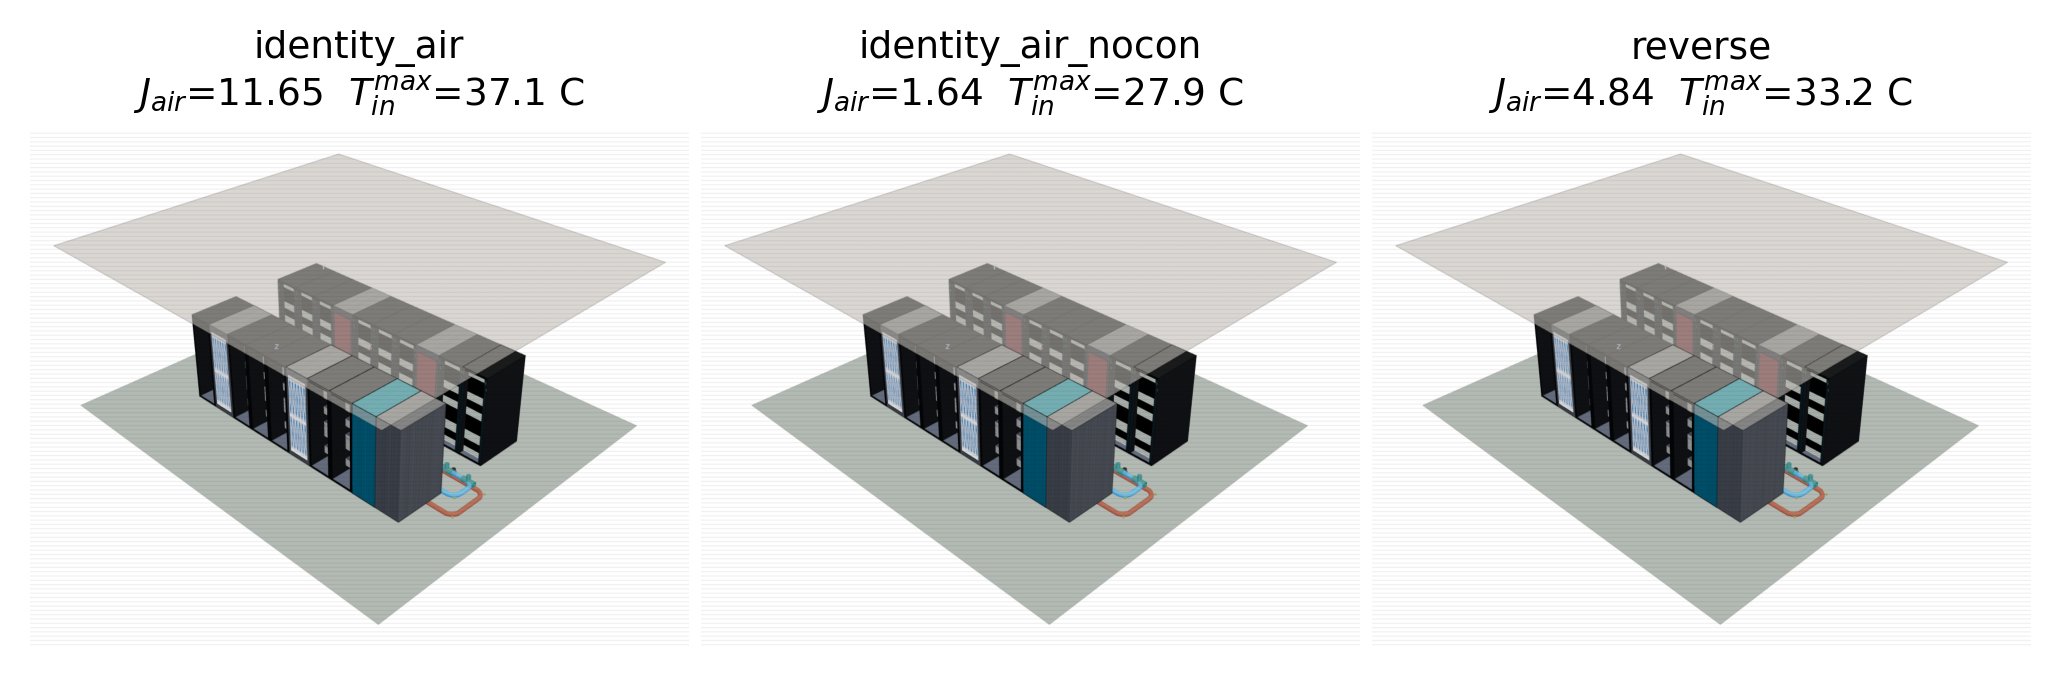
\includegraphics[width=0.94\textwidth]{figures/plate_containment_iso.png}
\caption{Three designs of one room.  Left to right: all racks air-cooled with
cold-aisle containment as authored in the production project; the same design with the
baffles removed; and the reversed placement---which is not only a placement, since the
generator also raises the ACU supply temperature to the catalogue maximum ($22$\,C
against $14$\,C), so the third panel confounds a permutation with a supply-temperature
change.  The design that isolates placement ($3.85$\,K per rack, \S\ref{sec:env}) is a
different one and is not on this plate.  \textbf{What the pixels cannot show:} the
frontend draws no containment baffles, and \texttt{figure\_diff.py} measures panels 1
and 2 at max channel difference $11/255$---\emph{inside} the $8$--$13$ spread of repeat
captures of one scene---although their physics differs by $9.0$--$9.2$\,K on the maximum
rack inlet.  Placement of visually identical racks is invisible here for the same
reason.  Ledger rows (11) and (25).}
\label{fig:containment}
\end{subfigure}\\[2pt]
\begin{subfigure}[t]{\textwidth}
\centering
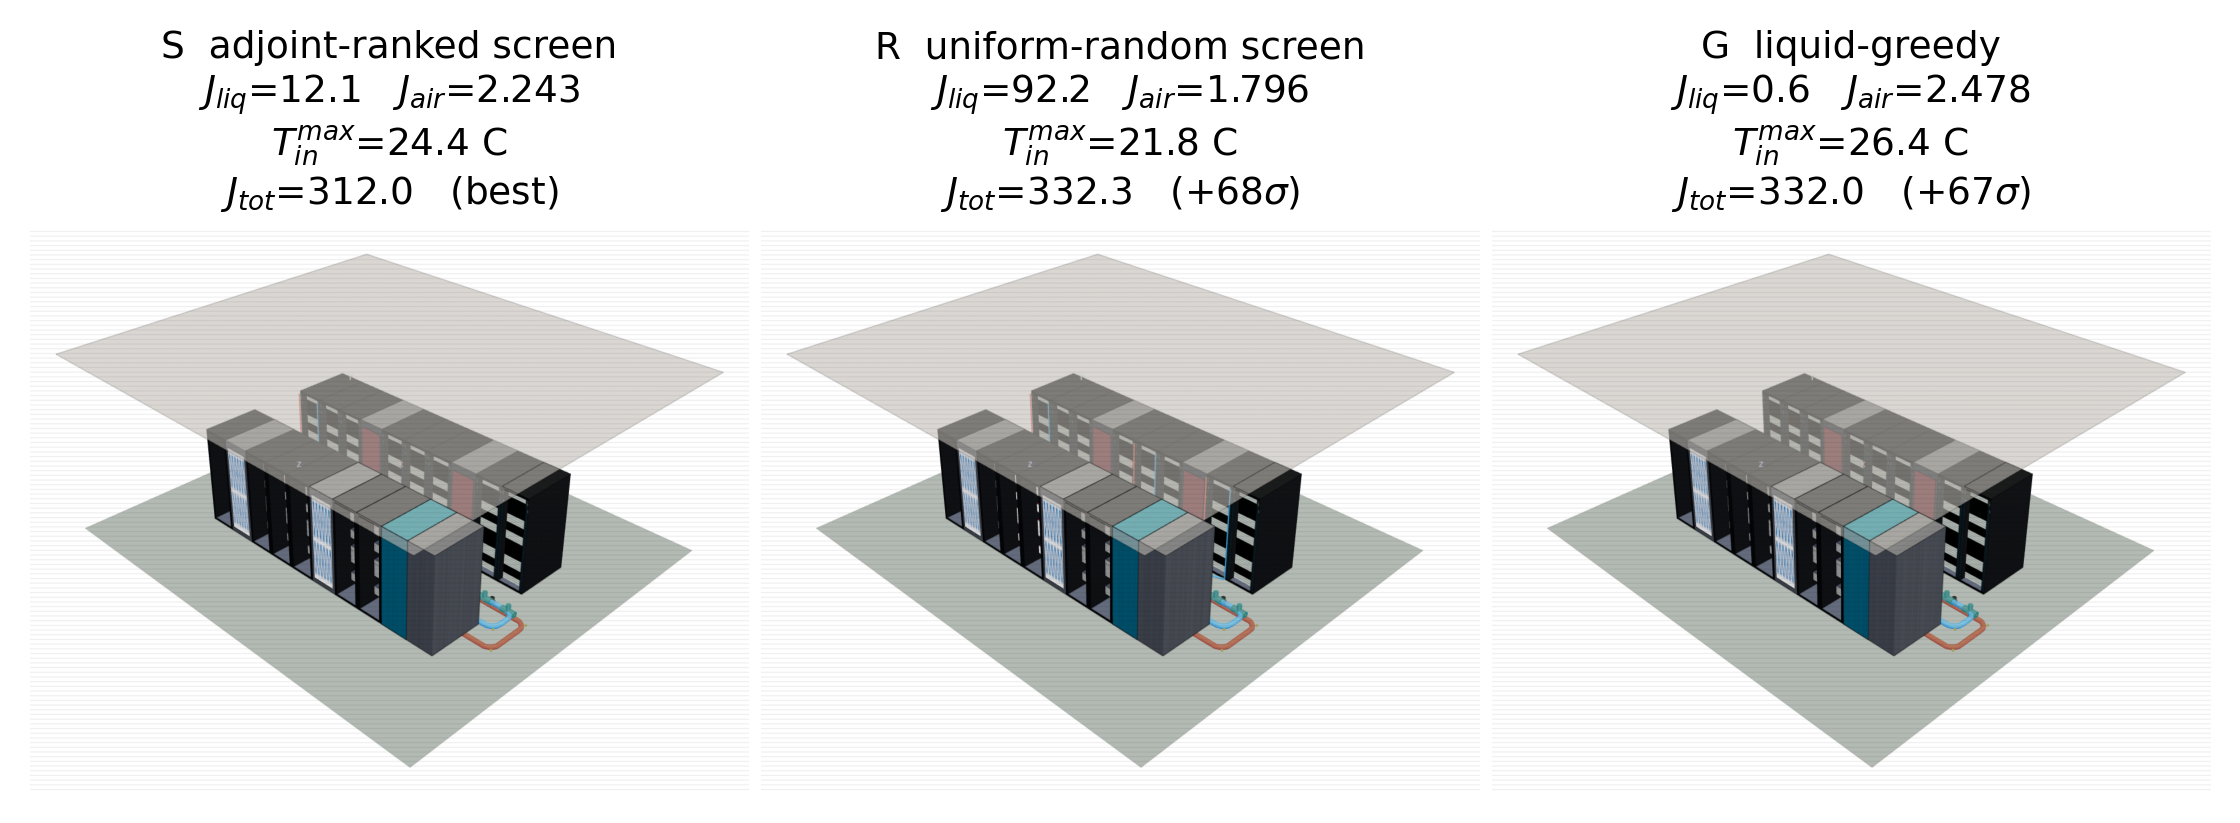
\includegraphics[width=0.94\textwidth]{figures/plate_search_iso.png}
\caption{The designs the three search arms selected on task 900050, the task whose
replicate-averaged S$-$R margin is closest to the median across the eight; the rule does
not determine it uniquely, since 900050 and 900054 are equidistant at
$3.4445\times10^{-1}$ and iteration order breaks the tie.  $\Jliq$ is the row stored
during the run; $\Jair$ the mean of three fresh full-chain re-evaluations;
$T^{\max}_{\mathrm{in}}$ recomputed from the archived probe payload; $\sigma$ the margin
over the best arm in units of the pooled replicate sd.  G's selection sits at
$\Jliq = 0.6$, the all-air degenerate basin: its liquid-greedy descent removed almost
all heat from the water loop, which is why its air objective and inlet temperature are
the worst of the three.}
\label{fig:search}
\end{subfigure}
\caption{Both plates are rendered by the simulator's own web frontend (HTML editor,
hardware WebGL, canvas only); annotations are read back from the archived probe records.
A figure from this pipeline is a \emph{view} of the room, not an encoding of the design
vector: the quantitative comparison lives in the annotations and tables, and
\S\ref{sec:figures} states what the renderer cannot draw.}
\label{fig:plates}
\end{figure*}



\begin{table}[!t]
\centering
\footnotesize
\setlength{\tabcolsep}{3pt}
\begin{tabular}{lrrrrrr}
\toprule
task & S & R & G & S$-$R & S$-$G & G$-$R \\
\midrule
900048 & 278.97 & 333.64 & 330.40 & $-54.67$ & $-51.42$ & $-3.24$ \\
900049 & 310.39 & 313.43 & 306.02 & $-3.03$ & $+4.37$ & $-7.40$ \\
900050 & 311.68 & 331.92 & 331.72 & $-20.24$ & $-20.04$ & $-0.20$ \\
900051 & 279.74 & 303.41 & 306.61 & $-23.66$ & $-26.87$ & $+3.21$ \\
900052 & 293.76 & 306.80 & 284.43 & $-13.03$ & $+9.34$ & $-22.37$ \\
900053 & 303.25 & 306.78 & 276.72 & $-3.53$ & $+26.53$ & $-30.07$ \\
900054 & 277.93 & 297.56 & 302.30 & $-19.62$ & $-24.36$ & $+4.74$ \\
900055 & 267.07 & 318.35 & 303.29 & $-51.28$ & $-36.22$ & $-15.07$ \\
\bottomrule
\end{tabular}
\caption{Best $\Jtot = \Jliq + 133.7\,\Jair$ per arm per task, lower is better.
Every arm billed and scored exactly 24 evaluations.  Wins out of 8, one-sided
exact sign test in parentheses: S$>$R \textbf{8} ($p = 0.0039$), S$>$G 5
($p = 0.3633$), G$>$R 6 ($p = 0.1445$).  Values are as billed; the
replicate-averaged re-measurement of the selected designs changes the median
S$-$R margin by less than $1.4\%$ (95\% CI; the two margins closest to the floor
move $3.03 \to 3.00$ and $3.53 \to 3.68$) and changes no win count.}
\label{tab:e11b}
\end{table}

\begin{table}[!t]
\centering
\footnotesize
\setlength{\tabcolsep}{2.5pt}
\resizebox{\columnwidth}{!}{%
\begin{tabular}{lccccc}
\toprule
wins out of 8 & $\lambda = 33.4$ & $\lambda = 93.1$ & $\lambda = 133.7$ (used) & $\lambda = 180.4$ & $\lambda = 534.8$ \\
\midrule
S vs R & 8 & 8 & \textbf{8} & 5 & 3 \\
S vs G & 1 & 5 & \textbf{5} & 6 & 7 \\
G vs R & 8 & 8 & \textbf{6} & 3 & 0 \\
\bottomrule
\end{tabular}%
}
\caption{Sensitivity of the arm ordering to the scalarization weight, recomputed
offline from the stored $(\Jliq, \Jair)$ pairs by \texttt{derive\_review.py}.
$93.1$ and $180.4$ are the two pooled regression estimates that bracket the
exchange rate, derived later in this section; the ordering inverts as $\lambda$
moves across that
range, and S versus R falls from $8/8$ to $3/8$ at the sweep's upper endpoint
($\lambda = 534.8$), which is the count the text cites; the $5/8$ an earlier caption
called the upper endpoint is the $\lambda = 180.4$ column, the inverse-regression end of
the bracket.  The sweep is descriptive and was not used to choose
$\lambda$.}
\label{tab:lambda}
\end{table}

\begin{table}[!t]
\centering
\footnotesize
\setlength{\tabcolsep}{4pt}
\resizebox{\columnwidth}{!}{%
\begin{tabular}{lcccc}
\toprule
decision block & edits & $\rho$ median & $\rho$ min & sign \\
\midrule
diameter (affine in $1/D^5$)   & 223 & $1.000$ & $0.999$ & $1.000$ \\
placement (affine in length)   & 316 & $0.990$ & $0.980$ & $0.924$ \\
assignment (inside the solve)  & 224 & $\mathbf{0.166}$ & $0.043$ & $\mathbf{0.679}$ \\
\bottomrule
\end{tabular}%
}
\caption{E13: Spearman $\rho$ between the adjoint's first-order prediction of
$\mathrm{d}\Jliq$ and a fresh re-solve, over the single-edit
neighbourhood of eight held-out tasks of the shipped benchmark (placement capped at $40$
moves per task), against the relaxed
re-solve.  \textbf{The assignment row is the all-edits $\rho$ and is not the number this
paper relies on:} half of that neighbourhood is a structural no-op, and \S\ref{sec:relax}
reports the informative half beside it.  Against the hard one the substance is unchanged (diameter $0.936$, placement
$0.994$, assignment $0.166$).  The pre-registered gate---sign $\ge 0.90$ pooled and
$\rho \ge 0.9$ on $\ge 6$ of $8$ tasks per block---\textbf{fails on assignment} and
passes on the other two; the failure is published, not dropped.  Generated from
\texttt{results\_e13.json}---produced by
\texttt{ddl/case/benchC/E13\_fullrank\_ranking/run.py}---by \texttt{measure\_e13.py}; no
number here is typed, and \texttt{check\_tracked\_records.py} fails if this record and the
manuscript disagree.}
\label{tab:e13}
\end{table}

\paragraph{Half the diameter neighbourhood does nothing, and Table~\ref{tab:e13} reports
that it does something.}
E13 calls an edit degenerate when the adjoint's prediction \emph{and} the measured effect
are both exactly zero.  On assignment that finds $112$ of $224$ edits---the air-cooled
half, which has no liquid branch, so both are zero and the accounting is right.  On
\textbf{diameter it finds none}, which reads as a fully informative block.  It is not one:
$111$ of the $223$ diameter edits leave the \emph{hard} objective exactly unchanged, while
the relaxation reports a nonzero effect on all $223$.  The block is half inert physically
and wholly sensitive in the surrogate, and those are different statements that one word was
collapsing.  Placement shows the same asymmetry at a smaller scale---$52$ of $316$ edits
hard-inert against $12$ relaxed-inert---and assignment shows none of it, because there the
relaxation and the physics agree about what is inert.

So the relaxation is \emph{not} invariant on coordinates the hard physics is invariant on,
and the size of that spurious sensitivity is already measured elsewhere in this paper: it
is what separates arm D's design from the adjoint search's on the relaxed objective
($1.07$--$1.24\times10^{-3}$ relative, below the $1.6\times10^{-3}$ closure floor) while
the two are bitwise identical on the hard one.  The three findings---the closure floor, the
arm-D gap and this---are one phenomenon, and ``physically closed'' is licensed by the
closure measurement over feasible designs rather than by invariance on inert coordinates.

The adjoint's ranking survives it.  On the $112$ hard-informative diameter edits
$\rho = 1.000$ with no task negative, against the constant rule's $+0.868$ on the same
subset ($+0.695$ over all $223$, where the inert half dilutes it), so this is a limit on
the relaxed objective and not on the gradient.  All of it is read from
\texttt{reanalysis\_degeneracy.json}'s \texttt{n\_measured\_zero} per block and objective by
\texttt{measure\_e13.py}; nothing here is typed.

\paragraph{The first clause passes and the second fails.}
S beats R on \textbf{eight of eight} tasks ($p = 0.0039$).  S beats G on only
\textbf{five of eight} ($p = 0.36$), so the gate as written is \textbf{not}
satisfied.  Neither pre-registered branch covers that landing---the negative
branch was written as ``S cannot beat R'', and S does---and the gap is recorded
rather than resolved after the fact.  G beats R on six of eight ($p = 0.14$),
which the corrected test does not support either.

The null result against G has two measured confounds and one withdrawn
explanation.  An earlier draft attributed it to the scalarization: $\lambda$ was
set to the measured exchange rate, so $\Jtot$ is approximately invariant to the
cooling split, so moving heat between the two oracles---exactly what a cooling
flip does and exactly what G optimises---is nearly free in $\Jtot$ and G harvests
most of the available gain while ignoring the air side.  That reading holds only
to first order at the tangent point and the winners sit far from it: at
$\lambda = 133.7$ the liquid term is $220\%$ of the net S$-$R margin
($-415.0$ against $+226.0$), so $\Jtot$ is not approximately invariant over the
range these searches actually traverse, and the mechanism is withdrawn with the
decomposition that withdraws it.  What remains measured is that every contrast
involving G is confounded---with \emph{depth} (24 single-bill steps against S
and R's 8 three-bill steps) and with the \emph{all-air basin}, where G spent
$73\%$ of its evaluations at a $\Jliq$ $17.6$--$19.5\times$ below any mixed design
in this record.
\textbf{The informative contrast is
oracle versus no-oracle, not policy versus policy}: both arms that consume the
gradient beat the arm that has none \emph{on the liquid objective}; G versus R is
6/8 ($p = 0.14$), which the corrected test does not support; and S versus G is 5/8,
so the two gradient-consuming arms are indistinguishable from each
other.  What the paper may claim is that at $B = 24$ a production solver with an
exact adjoint used as a surrogate beats uninformed screening \emph{on the liquid
objective, and only on the block whose neighbourhood is informative}---on assignment it
does not, and on diameter a constant design that is never searched for ties it
(\S\ref{sec:relax}); what it may not
claim is that batch screening beats myopic greedy descent on that surrogate.

\paragraph{Common units.}
The slope ratio puts the two costs in common units---and the ratio the campaign
actually used does not quite equal the ratio the fits give.  Fitted, it is
$184.3/1.386 = 133.0$; the pre-registered $\lambda = 133.7$ was computed as
$184/1.376$ from the rounded values quoted in the plan, and the plan's $1.376$ is a
transcription of a slope that fits as $1.386$.  Nothing is re-scored at $133.0$:
every record in this campaign used $133.7$, and changing the weight now would be
choosing it after seeing the data, so $133.7$ stands and the $0.5\%$ discrepancy is
defect (13).  At $\lambda = 133.7$ the scalarization
$\Jtot = \Jliq + \lambda\,\Jair$ is stationary in the cool split \emph{to first
order at the tangent point}---the two slopes cancel there by construction---and
sensitive to efficiency on both sides.  That cancellation is local and not global,
and \S\ref{sec:search} measures how far from local: over the eight tasks the
liquid term contributes $220\%$ of the net S$-$R margin at this $\lambda$
($-415.0$ against $+226.0$), so no global invariance of $\Jtot$ to the heat split
may be inferred from it.  At $\lambda = 1$ it degenerates (one
cool flip saves $\sim18$ of $\Jliq$ for $\sim0.16$ of $\Jair$, so ``move
everything to air'' dominates and the expensive oracle stops mattering).  We
disclose that $\lambda$ was set from the measured exchange rate, with the pilot
that motivated it, rather than presented as an a priori choice; sensitivity over
$\{33.4,\allowbreak 133.7,\allowbreak 534.8\}$ is recomputed offline from stored $(\Jliq, \Jair)$
pairs at zero extra CFD cost.

\paragraph{What the renderer cannot draw, in full.}
Both plates are rendered by the simulator's own web frontend---the stable single-file
HTML editor---through its project loader, on hardware WebGL (ANGLE over Vulkan), clipped
to the canvas; the figures, their provenance and the measurements behind every claim in
this paragraph are in Appendix~\ref{sec:figures}.  Three things a reader needs before
looking at them.  The frontend draws \emph{no} containment baffles, so the two panels of
Figure~\ref{fig:containment} whose physics differs by $9.0$--$9.2$\,K on the maximum rack
inlet are, as images, inside the noise of re-capturing one scene---measured by a
committed gate, \texttt{figure\_diff.py}, at max channel difference $11/255$ against a
repeat-capture spread of $8$--$13$.  Placement of visually identical racks and ACU
supply temperature are invisible for the same reason, while cooling technology is not
(max $76$--$188$).  And what is archived beside each image is five scalars, not a
histogram: the shell was never actually made translucent, and the raster leaves more
than the ``$\pm1$ LSB'' an earlier draft claimed.  A sentence asserting that a wrong
camera moves ``more than $1\%$ of pixels by more than $64/255$'' is withdrawn---no
control was ever run, and the largest real design difference on record is $0.025\%$
above that threshold (ledger row (25)).

\section{The agent arms in full, and why placement has no cheap opponent}
\label{app:agent}

\paragraph{The E12 curve.}  Regret medians on the hard network, from
\texttt{records/e12\_agent\_result.json}.  Each block is read from both \texttt{log.jsonl} and the
arm's stdout log and the extractor fails on disagreement; it reports $0$ mismatches on both arms,
so no number here rests on one source.  Feasible rates travel with the regrets because an
improvement bought with illegal designs is not one, and a split containing an infeasible task has
an uninterpretable \emph{mean}---its $10^9$ penalty puts \emph{ood}'s at $2.5\times10^6$---so only
medians are quotable there (Amendment 30.1d).

\begin{center}
\begin{tabular}{lrrrrrr}
\toprule
& \multicolumn{3}{c}{adjoint-coupled (ste)} & \multicolumn{3}{c}{scalar reward (grpo)} \\
\cmidrule(lr){2-4} \cmidrule(lr){5-7}
step & val & test & ood & val & test & ood \\
\midrule
$0$ & +0.0077 & +0.0107 & +0.0042 & +0.0077 & +0.0107 & +0.0042 \\
$50$ & +0.0707 & +0.0648 & +0.0749 & -0.0027 & +0.0015 & +0.0045 \\
$100$ & +0.0157 & +0.0346 & +0.0588 & -0.0027 & -0.0000 & +0.0038 \\
$150$ & +0.0399 & +0.0277 & +0.0244 & -0.0050 & -0.0029 & +0.0045 \\
$200$ & +0.1368 & +0.0308 & +0.1152 & -0.0072 & -0.0128 & +455.3878 \\
\bottomrule
\end{tabular}
\end{center}

At the final step the feasible rates are ste $1.000/1.000/1.000$ and grpo
$1.000/0.875/0.375$ on val/test/ood, against $1.000/1.000/0.750$ at initialisation.
Neither arm records an OOM event, and both ran the $200$ steps they were
pre-registered to run, so the validity audit V0 passes on both with no reasons recorded---but it
passes under Amendment 29's mechanistic redefinition, and under A11.6 as \emph{literally}
pre-registered ($\texttt{sf} = 0$ on $0\%$ of logged epochs, zero tolerance) the scalar-reward arm
\emph{fails}: its score-function gradient is exactly zero on $15$ of $200$ steps, $7.5\%$, every one
of them a step on which the Amendment-19 guard zeroed the rescale because the task gradient was
degenerate.  Those steps contributed no update at all, so the arm improved on $185$ effective steps
of $200$---a limitation on its result and not a defence of it.  The coupled arm logs no
score-function gradient and is not subject to that clause.  Amendment 29 relaxed a pre-registered
zero tolerance into an unbounded report, and the audit's guard branch still has no upper bound, so
an arm with $\texttt{sf} = 0$ on every step but the last would pass clause 3 while failing clause 5.
Both readings are computed side by side in \texttt{records/e12\_v0\_audit.json}, because a gate that
reports only the reading under which it passed has chosen its own verdict.  The scalar-reward arm logs
$65$ degenerate-gradient steps of $200$, each with its rescale zeroed, which is the
Amendment-19 guard firing on a step that had no signal and not the float32 bug; the coupled arm
logs none, and one step whose rescale falls in $[10^6, 10^{11})$---step $1$, the
first, where the EMA normaliser is initialised from its own first batch---with no step anywhere in
the repository at or above the $10^{11}$ saturation signature.

\paragraph{Why placement has no cheap opponent.}  \S\ref{sec:relax} quotes E15's measurement; this
is the argument behind it.  The slot-length tensor $L[i,k,s]$ has \emph{exactly zero} spread over
the rack index on all $8$ tasks, because a pipe run is a property of the slot and the CDU
and not of the rack standing in the slot, so $L[i,k,s] = B[k,s]$ and
$\sum_i\sum_k B[k,\pi(i)] = \sum_k\sum_s B[k,s]$ for every permutation $\pi$.  Total relaxed pipe
length is therefore a permutation invariant, and the unweighted geometric prior that Amendment
30.3 first registered as arm G scores all $182$ swaps of a task within a relative range of
$5.6\times10^{-16}$---withdrawn for a measured reason, and recorded so the withdrawal is
checkable.  What E11f reported as a ``rank-one pipe-length heuristic'' reproducing the adjoint at
$\rho = 1.0$ consequently draws all of its information from the length sensitivities
$\partial\Jliq/\partial L[i,k]$, which are hydraulic; the name points at the wrong source of
information.  Those sensitivities cost $1 + 2NK = 85$ central differences per state against
one backward pass, and that ratio is the entire content of the adjoint's advantage on this block.
It is a \emph{count}, and the price is smaller: one forward+backward solve measures $14$\,ms
against $8.4$\,ms forward-only, an overhead of $1.7\times$, so those $85$ central differences cost
$51\times$ one backward pass in wall clock rather than $85\times$.  Both are recorded in
\texttt{records/oracle\_costs.json}, measured over $5$ repeats with a $14.9\%$ spread at a logged
load average of $24$ on $64$ cores, because a solve timed under load is not the number a solve
timed on an idle box gives.  A count and a price are the two numbers most easily substituted for
one another, and E15 charges its arms in the count.

Per-state agreement between the heuristic and the adjoint (G17, computed off-budget so that
measuring it cannot move the quantity under study) is a median $\rho$ of $0.957$ for the stale
linearisation---only $6.8\%$ of its states reach $0.99$---and $0.99998$ for the current
one, where $100\%$ do.  The stale model ranks worse and searches to the same design, so on
placement it is budget, not ranking accuracy past $\rho \approx 0.96$, that decides the outcome.

\section{The search experiments in full: arms, budgets and mechanisms}
\label{app:search}

Body \S\ref{sec:relax} states the three verdicts; this is the harness behind each,
moved here whole rather than paraphrased, so that every number the gates anchor on is
the sentence that was written when the measurement was made.

\paragraph{A search on each block separately---and the design that beats it.}
E13 ranks a neighbourhood; E14 runs the search.  Restricting the move generator to one
block at a time, \textbf{three} arms bill the same $24$ evaluations per task:
\textbf{S} ranks candidates by the adjoint's predicted
$\mathrm{d}\Jliq$, \textbf{R} bills them uniformly at random, and \textbf{C} bills them in
order of target index alone---the constant rule of the previous paragraph, which on
diameter is simply ``use the largest pipe''.  The three see the same pool at step $0$ and,
because each arm's pool is enumerated from its \emph{own} current design, different pools
after it; what the record asserts is equal billing, $24/24/24$ with zero skipped solves on
every scored task, and an earlier ``identical candidate pools'' claimed more than that.
Beating R is nearly free; C is the opponent a ranking correlation of $0.867$ demanded.

\textbf{D} is not a search.  It writes down the coordinatewise-minimum target design---on
diameter, the largest pipe on every rack, which follows from the model's own $1/D^5$
resistance form without solving it---and bills \emph{one} evaluation.  Its budget is
unequal by design, so every contrast involving D is labelled unequal-budget and is about
information and design quality, never about cost.

One task of the eight is \emph{refused} rather than scored: seed 910034's base design does
not converge at this revision (hydraulic residual $4.5\times10^{-3}$ against a $10^{-9}$
tolerance, deterministically), although the
archived first run of this case completed it.  The refusal \emph{costs} this paper a win:
in the archived two-arm run 910034 was an S victory on diameter at $-18.9\%$, so diameter
was $8$ of $8$, $p = 0.0039$ one-sided, and is now $7$ of $7$, $p = 0.0078$.  Every
statistic below is therefore over \textbf{seven} tasks, a task that cannot solve is
recorded with its error rather than dropped silently, and the sensitivity of the published
\emph{S-versus-R} numbers to the eighth is measured in
Appendix~\ref{app:derivations}: $22$ numbers move and \emph{no verdict does}.  That script
reads the two-arm archive and covers S versus R only, so the S-versus-C, C-versus-R and
every S-versus-D number are \emph{not} covered by it; and one of the $22$ moves is the
count behind ``negative on five of eight tasks'' below, which is four of seven on the
tasks that reproduce.  The other seven reproduce their archived base objective to a worst
relative deviation of $6.4\times10^{-16}$, about $5$ ULP---an earlier ``one ULP (relative
$1.3\times10^{-13}$)'' was neither, and the script it cited reports that \emph{no} base
objective reproduces bitwise.  No thread sweep was ever run, so the earlier ``at every
thread count from $1$ to $64$'' is deleted rather than repaired.

On \textbf{diameter} the ordering among the three searched arms is $S \succ C \succ R$ on
all seven tasks and on both networks: S beats C \textbf{$7$ of $7$} (one-sided
$p = 0.0078$, two-sided $0.0156$; median margin $-5.07\%$, range
$-9.24\%$ to $-4.45\%$), C beats R $7$ of $7$ ($-11.42\%$), and S beats R by $-18.64\%$,
with the same $7$ of $7$ when each arm's final design is re-scored by the \emph{hard}
network.  \textbf{D matches S, and on the objective that measures what a design costs it is the
same design.}  On the \emph{hard} network the two are \textbf{bitwise identical} on
$7$ of $7$ tasks.  On the relaxed objective---the one this campaign's primary statistic is
defined on---D is lower by a median $+0.117\%$ against S (range $+0.107\%$ to $+0.124\%$),
so S scores $0$ of $7$ under the convention that ties are losses for the arm claiming
superiority.  That gap is $1.07$--$1.24\times10^{-3}$ relative and \emph{every one of the
seven} sits below this campaign's own median closure floor of $1.6\times10^{-3}$ over the
$311$ feasible designs of the shipped benchmark, so it is inside the relaxation's measured
error bar rather than outside it.  The six coordinates the two designs differ on are
on coordinates that are exactly the air-cooled racks, which have no liquid branch: the relaxation is charging
about $0.1\%$ for a decision the hard physics ignores, and that is a property of the
relaxation worth knowing rather than a design difference---one E13's own records already
measure at $111$ of $223$ diameter edits (Appendix~\ref{app:derivations}).  D also beats C $7$ of $7$ at a
median $-5.17\%$---\emph{more} than S's $-5.07\%$ over the same opponent, at $24\times$
the billing---and beats R $7$ of $7$ at $-18.74\%$.  On \textbf{assignment}
nothing works: S beats R \textbf{$1$ of $7$}
(one-sided $p = 0.992$), S beats C $2$ of $7$ and C beats R $2$ of $7$, so uniform billing
is the best of the three searched arms, the gradient-free rule beats the adjoint on
$5$ of $7$, and S's single win over R is a $0.08\%$ margin.  D's constant assignment is
not a legal design---every rack on one CDU---and the hard network marks it infeasible on
all eight tasks, three of them at the $10^9$ solver-failure sentinel; S beats it $5$ of $7$
there, which is reported and supports nothing.  The hard network drops one
further task on assignment---seed 910036, where R's final design is infeasible at
$10^9$---which is recorded per contrast rather than silently reducing the denominator from
$7$ to $6$.  No air evaluation is spent, so this is a weight-free liquid-side result:
each searched arm performs $32$ liquid solves per task, of which $24$ are billed
candidates, and R and C are handed the gradient and ignore it, which is generous to
\emph{their opponents} rather than to them.

\paragraph{Why the exact gradient loses: not blindness, but eight steps.}
The two available explanations imply different papers, so the run measures which holds.
On every scored task S's final diameter vector differs from D's on exactly \textbf{six} of
fourteen coordinates and has exactly \textbf{eight} of fourteen racks at target---one
accepted move per step over eight steps.  On those six the adjoint's predicted
$\mathrm{d}\Jliq$ is \emph{never} exactly zero ($0$ of $42$ coordinate measurements) and is
always correctly signed, so the gradient is not blind; four of the six correcting moves
were simply never billed.  What it gets wrong is magnitude: against the finite jump its
first-order prediction understates the improvement by a median factor of $4.26$ (range
$4.21$--$4.28$), which is why moves worth $0.01$ rank behind moves worth $4$ and the search
terminates before converting them.  On assignment the opposite holds---four to six of the
nine to eleven differing coordinates \emph{are} exactly zero, the inert air-cooled
half---so the two blocks fail for different reasons and only one is an information
failure.

\paragraph{Placement, the third block, and the opponent that is exactly degenerate.}
Diameter and assignment are two of the three blocks E13 ranked.  The third is placement---a
permutation, so no constant vector is even legal---and it is the block every earlier search
in this campaign actually exercised while no search ever gave it a matched-budget opponent.
E15 supplies one, and first measures that the cheapest geometric prior is not weak but
\emph{exactly degenerate}: the slot-length tensor $L[i,k,s]$ has zero spread over the rack
index on all eight tasks, because a pipe run is a property of the slot and the CDU and not
of the rack standing in it, so total relaxed pipe length is a \emph{permutation invariant}
and ranking all $182$ swaps of a task by its change gives a score of relative range
$5.6\times10^{-16}$.  What E11f reported as a ``rank-one pipe-length heuristic'' matching
the adjoint at $\rho = 1.0$ therefore draws \emph{all} of its information from the length
sensitivities $\partial\Jliq/\partial L[i,k]$, which are hydraulic, and which it buys with
$1 + 2NK = 85$ central differences where the adjoint returns them in one backward pass.  The
name points at the wrong source of information, and the geometry contributes nothing.

E15 charges four arms in \emph{total solver calls}, forward and backward alike---the
correction E14 needed, whose ``matched billing'' counted billed candidates while
\texttt{liquid\_state} ran \texttt{autograd.grad} for every arm including the gradient-free
ones.  Over budgets $\{128, 256, 512\}$ on the seven tasks that solve: \textbf{S} (adjoint)
\emph{ties} \textbf{F1} (sensitivities estimated once at the base design, then left stale) on
$7$ of $7$ at every budget, maximum relative difference $1.9\times10^{-15}$ on the relaxed
and the hard network alike; beats \textbf{R} (uniform) $7$ of $7$, $p = 0.0078$; and beats
\textbf{F2} (sensitivities re-estimated at every state) $7$ of $7$ at $128$ and $256$, tying
it at $512$.  The quantity E15 exists to measure is the budget each arm needs to reach the
optimum they all eventually reach: S $128$, F1 $128$, F2 $512$, and R on only $2$ of the $7$
tasks at all, at $128$ and $256$, never on the other $5$.  So keeping the linearisation \emph{current} costs four times the budget,
because it costs $85$ solves per state against one backward pass---and keeping it \emph{stale}
costs nothing in design quality, because F1's ranking agrees with the adjoint at a median
per-state $\rho$ of only $0.957$ ($6.8\%$ of its states reach $0.99$, against $100\%$ for F2
at $0.99998$) and reaches the same designs anyway.  On placement, ranking accuracy past
$\rho \approx 0.96$ does not decide the outcome; budget does.

\paragraph{What survives.}
Both predictions E13 made from the ranking measurement hold, including the negative one,
and so does the one made about the constant ranking rule before it was run.  What does not
survive is the inference from a perfect ranking to a better design, and on diameter it could
not have: D's vector is the benchmark's own \texttt{diam} reference field on
\textbf{$7$ of the $8$} tasks, so the optimum was in the data file, and the base design is
$14$ single-coordinate changes from it while the harness accepts one move per step over
eight steps.  \textbf{Diameter therefore has no measurable headroom above a design that
can be written down}, and it is re-scoped as a gradient-\emph{correctness} test rather
than a search test.  What the adjoint does buy there is a better choice of which eight of
the fourteen changes to make: at $32$ solves it beats every gradient-free opponent tested at
that budget, by $5.1\%$ over the constant ranking rule and $18.6\%$ over uniform random, and
by more over a systematic sweep, a finite-difference ranking and a refitted least-squares
surrogate.  On placement the same shape recurs with a different mechanism: the adjoint is not
beaten but it is \emph{matched}, exactly and at equal total cost, by a heuristic whose model
is stale---and the only thing exactness buys is that a \emph{current} model becomes
affordable at all, at a measured $4\times$ budget penalty for the alternative.  The
transferable part is methodological and it is a negative: a ranking diagnostic computed on a
\emph{single} design, at the cost of one gradient, correctly identified the block where the
gradient is half-blind---and did \emph{not} identify the block where an exact,
correctly-signed gradient still loses to a one-line constant, because that failure is in the
search's step budget rather than in its information.  ``The adjoint is exact'' therefore has
to be checked against a design that can be written down, and against an opponent that can
afford to be stale, not only against a ranking correlation.  It is a diagnostic over
\emph{three} blocks, on eight load draws of one template; it is hypothesis-generating
evidence about where a gradient pays, not a validated general-purpose gauge.

\section{Derivations, gates and withdrawn numbers}
\label{app:derivations}
Material the body states the conclusion of and the records carry the derivation of.  Nothing here is optional reading for a reader who wants to check a number: the $\lambda$ conditioning, the $p$-value defect and the archive-link proof are the three places where a claim in the body rests on an argument longer than the body has room for.

\paragraph{One task of eight no longer solves, and nothing turns on it.}
E13 and E14 both score the same eight held-out tasks, and one of them cannot be re-scored.
\texttt{probe\_reproducibility.py} re-solves all eight base designs at this revision:
seven reproduce their archived $\Jliq$ base objective to a worst relative deviation of
$6.4\times10^{-16}$, about $5$ ULP, and seed 910034 raises
``hydraulic solve did not converge (residual $4.538\times10^{-3}$)'' against a $10^{-9}$
tolerance---deterministically, from the unpatched \texttt{run.py} at the revision that
produced the record, with the solver unchanged since 2026-09-16, \texttt{data\_C}
unchanged since 2026-09-17 16:40.  Two clauses an earlier draft carried here are
deleted rather than repaired: no thread sweep was ever run, and no script compares the
compiled slot lengths against the cached copy on disk.  So the deviation is not thread noise: it is one design whose damped-Newton
homotopy lands on the wrong side of its own tolerance.  That task was already the marginal
one in the archived run, which recorded $5$ of its $96$ edits as solve failures.

The archived eight-task run of E14 reported diameter $8$ of $8$ ($p = 0.0039$) and
assignment $1$ of $8$ ($p = 0.996$, $1$ of $7$ hard).  \texttt{sensitivity\_task.py}
recomputes the published \emph{S-versus-R} statistics twice from the archives---over all
eight tasks and over the seven that still solve---because the comparison needs no
re-solving and so cannot be confounded by one.  Its scope is narrower than an earlier
draft's ``every published E13 and E14 statistic'': it reads the archived \emph{two-arm}
record and hard-codes the S-versus-R contrast, so the arm-C contrasts added by Amendment
24.3, the arm-D contrasts added by Amendment 26 and gates P3, G5, G6 and G7 are
\emph{not} covered by it, and cannot be---the eight-task archive predates both arms, so
their sensitivity to the eighth task is not computable from any record this campaign
holds.  One of the $22$ moves it does report is the count behind ``negative on five of
eight tasks'' in \S\ref{sec:relax}, which becomes four of seven on the tasks that
reproduce.  \textbf{22 numbers move and no verdict does}: diameter
becomes $7$ of $7$ at $p = 0.0078$ (gate G1 still passes), assignment stays a loss at $1$
of $7$, $p = 0.992$ (G2 still fails), E13's assignment $\rho$ over all edits moves
$0.166 \to 0.171$ and its informative-half $\rho$ $-0.193 \to -0.196$, and the pooled
sign agreement that fails the $\ge 0.90$ gate moves $0.679 \to 0.694$ and still fails.
Both runs are kept: the archived one because two review rounds read it, the re-run because
it is the one that carries the third arm.  A run that cannot solve a task now records it
with the error and refuses it from every tally under gate G7, rather than dying in a print
statement, which is the shape of defect (19).

\paragraph{Exactness and ranking usefulness are ordered oppositely, and only one of them
follows affinity.}
E10 gate 2 compares the implicit adjoint with central differences block by block, and the worst
per-block median over all $294$ coordinates is $1.45\times10^{-7}$: assignment $1.53\times10^{-10}$
($n = 42$), cooling fraction $3.66\times10^{-8}$ ($n = 14$), diameter $1.08\times10^{-7}$
($n = 42$), placement $1.45\times10^{-7}$ ($n = 196$).  The \emph{most} exact block is the one
that enters through the nonlinear Newton solve, by dividing a branch resistance coefficient by a
weight $w \in [C_{\min}, 1]$, and the \emph{least} exact is the one that enters affinely, through
pipe length.  Affinity therefore does not predict adjoint accuracy on this environment, and a
reader who took \S\ref{sec:relax}'s mechanism paragraph as a claim about accuracy would have it
backwards.  What affinity does track is the ranking statistic $\rho$ over \emph{finite} single
edits, which is a linearization error and a different quantity: an edit between one-hots is a
jump, not an infinitesimal, and the jump is large exactly where the decision enters by dividing a
coefficient inside the solve.  Both statements are supported by shipped records
(\texttt{records/e10\_adjoint.json} for the exactness ordering, \texttt{records/e13\_ranking.json}
for the ranking one), and the distinction is the reason \S\ref{sec:relax} says ``exact on all four
blocks, useful for ranking on placement and diameter only'' rather than collapsing the two.  It
also leaves the fourth block open: cooling fraction is the second most exact block and the only
one whose decision is intrinsically continuous, and no search in this campaign has ever been run
on it with a matched-budget opponent.

\paragraph{Scope, and what a single network instance can show.}
\emph{Scope of that exactness.}  Every number above comes from one record (E10): a
single seed (900048), one room, $14$ slots, three designs, $16.9$\,s of solves.  The
$1.45\times10^{-7}$ is therefore a claim about one network instance, not about the task
distribution---the $n$ beside each block ($42$/$14$/$42$/$196$) counts finite-difference
probes of that instance, not independent tasks.  Exactness of an implicit adjoint is a
property of the assembled system, so one instance is strong evidence for the code path,
but it is not $1.45\times10^{-7}$ across the benchmark.

\paragraph{Thirty-five single decisions, and why they are not the interesting ones.}
\paragraph{Does the gradient say anything?}
For 35 single decisions---slot swaps scored against the true hard re-solve, cooling steps
against the relaxed one---the adjoint's first-order prediction agrees in sign on all 35
and ranks them at Spearman $\rho = 0.999$.  Sign and rank are not magnitude: three of the
eleven hard-resolve swaps are predicted $18\times$, $26\times$ and $256\times$ too small
($-9.33\times10^{-4}$, $-6.18\times10^{-4}$, $-6.43\times10^{-5}$ against
$-1.64\times10^{-2}$ measured), so the agreement is about \emph{ordering}, which is all
\S\ref{sec:search} uses it for.  Those 35 are slot swaps and cooling steps, which is not where the question is
interesting.

\paragraph{Classifying a finite-difference outlier rather than discarding it.}
The single placement coordinate at
$6.3\times10^{-3}$ is classified, not discarded: its finite-difference error
\emph{grows} as $h$ shrinks ($3.4\times10^{-4}$, $6.3\times10^{-3}$,
$5.4\times10^{-2}$), the signature of a kink in the damped Newton solve's
data-dependent trip count, while genuine finite-difference noise shrinks like
$h^2$.  The gate passes only with zero unexplained outliers.

\paragraph{Selection bias, removed by re-measurement.}
Every arm's reported number is a \emph{minimum over 24 noisy evaluations}, which is
optimistically biased toward whichever arm's draws scattered downward.  We therefore
recover the design each arm actually selected from its archived compiled project---not by
replaying the search---and put it through the full chain three more times: 72 fresh
evaluations.  The pooled within-design replicate sd is $\sigma(\Jair) = 0.002237$
(48 dof), i.e.\ $\sigma(\Jtot) = 0.299$ at $\lambda = 133.7$; that is $7.5\times$ smaller
than E8's uncontained repeat range read as a sigma ($0.0168$), and the gap is
\emph{unexplained}---the records do not support the obvious reading that the two
experiments sampled different design families.  Every margin below is quoted against all
three floors rather than the most convenient one.  De-biasing moves the median S$-$R
margin from $-19.93$ to $\mathbf{-19.98}$, a change of $-0.053 \pm 0.108$
(95\% CI $[-1.33\%, +0.80\%]$, i.e.\ $<1.4\%$); the two margins closest to the
propagated floor move $3.03 \to 3.00$ and $3.53 \to 3.68$ (A02); and this changes no
win count: S still beats R on eight of eight,
$p = 0.0039$.  The median margin is \textbf{66.8$\times$} the pooled replicate sd
($26.6\times$ the worst per-design sd, $8.9\times$ E8's uncontained range as a sigma)
against a pre-registered bar of $5\times$; the \emph{smallest} of the eight margins is
$10.0\times$ the pooled sd but only $4.0\times$ the worst per-design sd and
$1.34\times$ E8's range, so \emph{the smallest margin breaches the $5\times$ bar under
the most conservative floor}.  The gate was written against the pooled floor and passes
there; both are reported, because quoting only the favourable one is how a $5\times$ bar
becomes decorative.  All eight margins per arm are in Table~\ref{tab:e11b}, and all six
ratios come from \texttt{floor\_ratios.json}, computed by a committed script from the
E11c and E8 records; the third was $8.8$ in an earlier draft
against a record value of $8.91$, which is defect (12).  The designs the three arms
selected on the task whose margin is closest to the median are rendered in
Figure~\ref{fig:search} of Appendix~\ref{sec:figures}---though ``closest to the median'' does not pick one: with an even
number of tasks the median is the mean of the middle two, so 900050 and 900054 are
equidistant at $3.4445\times10^{-1}$ and iteration order breaks the tie, which is less
determinacy than an earlier caption's ``chosen by rule, not by appearance'' claimed.


\paragraph{A validity verdict that flips on an unexplained choice of noise floor.}
The re-evaluation that scores the GP-BO head-to-head carries a validity gate, D0: each
design's reproduce error---the freshly measured mean $\Jair$ against the value the original
run stored---becomes a $z$ against $\sigma\sqrt{1 + 1/R}$, and the measurement is declared
invalid if any $z$ exceeds $3.0$.  As shipped D0 used $\sigma = 0.002237$, E11c's pooled
within-design replicate sd, and one design of sixteen (900048/\texttt{B\_gp}/row6,
reproduce error $0.04101$) reached $z = 15.875$, so the whole measurement was judged
\textbf{invalid}.  But \S\ref{sec:search}'s limit (c) states that these designs are
uncontained and that ``the applicable floor is E8's uncontained one'', and that floor is
$0.01678$ in $\Jair$---\textbf{$7.5\times$ larger}, a discrepancy \S\ref{sec:search}
already reports as unexplained.  On the floor the paper says applies, the same design gives
$z = 2.117$ and D0 \textbf{passes}, with zero of sixteen designs over threshold.
\texttt{derive\_e11d\_d0.py} reads both floors from their records and emits both $z$'s, the
per-design table and the family-wise exceedance chance into
\texttt{records/e11d\_d0\_floors.json}, so every number in this paragraph is traceable to a
committed record rather than typed; as a self-check it reproduces the shipped $15.875$ to
three decimals.  It deliberately does \emph{not} flip the verdict to
valid: with two measurements of one oracle's noise disagreeing by $7.5\times$ for no
recorded reason, the conservative floor is the defensible one, so the verdict stands as
\emph{floor-dependent and unresolved}.  This was the only place in the campaign where a
single floor decided an outcome---every margin in \S\ref{sec:search} is quoted against all
three.

\paragraph{A reversed direction, introduced by a correction and inherited by the next
review.}
The passage in \S\ref{sec:related} that reports the GP-BO head-to-head said, in the
previous revision, that ``a GP Bayesian-optimization arm beats the adjoint-ranked screen on
$6$ of $8$ tasks'' and that the paper ``shows the opposite''.  Both halves were backwards.
The record's field is \texttt{D1.wins = 6} with \texttt{median\_margin\_Jtot = -24.4485},
negative in the screen's favour, and \texttt{wins\_ref = 2} for the baseline; the screen
wins six and the gate fails because the bar was seven.  The error was introduced while
incorporating a review finding about that sentence and was then repeated by the next review
round, which concluded from it that ``the method's only head-to-head is a loss''.  It is
ledger row (28), and the lesson is the one this campaign keeps relearning: a number carried
across by prose rather than read out of a record is wrong often enough that the direction,
not just the magnitude, has to be checked.  The two readings that are \emph{not} equivalent
to the headline are reported here rather than folded into it: weight-free over the
as-shipped visited sets the screen wins at every defined $\tau$ on $8/8$ tasks (descriptive,
not de-biased), and the $\lambda$ sweep gives $8/8$ at $\lambda = 33.4$ (below the
identified bracket), $6/8$ at the $133.7$ used, $5/8$ at $180.4$ and $1/8$ at $534.8$---the
same weight-dependence every other contrast in this paper shows.



\paragraph{The weight is not identified, and its interval was too narrow.}
$\lambda = 133.7$ is the slope ratio $184/1.376$ from the six-design pilot of
\S\ref{sec:tradeoff}, fixed before this run.  Re-estimating from the pooled 576 pairs
does not recover it: regressing $\Jliq$ on $\Jair$ gives $\lambda^* = 93.1$ and inverting
the other regression gives $180.4$, a factor of $1.94$ that is exactly $1/R^2$ at
$R^2 = 0.52$---the errors-in-variables identity, so neither is ``the'' rate and the two
\emph{bracket} it.  Appendix~\ref{app:results} tabulates what widens the bracket, all of
it computed by committed scripts: the 576 rows are clustered ($8$ tasks $\times\,3$ arms
$\times\,24$ self-selected evaluations), so a cluster-robust SE is $2.35\times$ the iid
one direct and $2.74\times$ inverse; task fixed effects barely move the bracket (factor
$1.81$) but arm fixed effects widen it to factor $6.26$, and per arm it is $5.8$ (S),
$4.5$ (G), $23.1$ (R), so the pooled bracket is the \emph{narrowest} available and is
partly an aggregation effect, not physics; and $133.7$'s own interval---two slopes fitted
to \emph{six} designs on four degrees of freedom---is the widest of all, $[0.6, 265]$ by
delta method, bootstrap $[63, 375]$, Fieller $[54, 7568]$, of which the pooled bracket
contains $63\%$.

\paragraph{The surrogate's value is regime-dependent, and the sweep may not re-choose the weight.}
Re-scoring the same visited designs at $\lambda \in \{33.4, 93.1, 133.7, 180.4,
534.8\}$---the two extremes, the two regression endpoints of the bracket below, and
the weight the campaign used---costs no CFD and inverts the arm ordering exactly
where \S\ref{sec:tradeoff}'s slopes say the objective changes hands
(Table~\ref{tab:lambda}).  As $\lambda$ grows the objective becomes air-dominated and
ranking by predicted $\mathrm{d}\Jliq$ goes from uninformative to actively harmful
(S versus R collapses $8/8 \to 3/8$); as $\lambda$ shrinks it becomes
liquid-dominated and pure liquid greedy wins everything (G versus R $8/8$, G versus
S $7/8$).  The sweep is descriptive and may not be used to re-choose $\lambda$: it
re-scores designs visited under a $\lambda = 133.7$ search, so the collapse at
$534.8$ happens under a bias \emph{against} S (mean regret against the best design
visited in that task: S $54.0$, R $3.7$) and is partly a steering artifact, while the
$8/8$ at $133.7$ is the number the re-measurement above had to de-bias.

\paragraph{The critical value that decides whether $133.7$ is outside the bracket.}
The script hard-codes $z = 1.96$,
justified by $574$ residual df---sound for residual df, unsound for a cluster-robust SE
with $G = 8$ clusters, where the reference is $t(7) = 2.3646$, a $20.6\%$ widening.  At
$t(7)$ the pooled inverse cluster interval is $[133.2, 227.6]$ and \emph{contains}
$133.7$, as does every fixed- and random-effects and per-arm inverse interval; only the
\emph{direct} ones exclude it either way.  The plan's ``except arm G's inverse interval''
is contradicted by its own record, which excludes nothing for arm S either
($[120.0, 454.6]$).  Per task, $133.7$ lies in the direct interval on $4$ of $8$ tasks and
the inverse on $2$ of $8$ \emph{under iid SEs}---the record's field names say
\texttt{\_iid}, an earlier draft's columns did not; clustered, the direct count is $5$ of
$8$.  The win count falls to $6/8$ inside the inverse interval and $5/8$ at its point
estimate $180.4$ (Table~\ref{tab:lambda}), which is what an unidentified weight predicts
and not evidence against the arm.  A cheap differentiable oracle therefore does not buy a
uniformly better design; it buys a better design \emph{on the scalarization whose weights
its own gradient measured}---and this paper cannot say which scalarization that is.

\paragraph{Why the all-liquid end of the cooling range is not an air-side cost.}
The $0.889$ end of \S\ref{sec:env}'s cooling range is the \emph{all-liquid} design, and a
liquid-cooled rack compiles to a \texttt{nonFan} chassis whose residual heat enters the room
through server plates at a fixed temperature, so the air oracle is close to blind to that
heat.  The $13\times$ ratio is evidence that the environment resolves the decision; it is not
evidence that $0.889$ is a meaningful air-side cost, and defect (3) is exactly the draft that
read it that way.  This is the qualifier A11.2(5) requires.

\paragraph{The per-block finite-difference maxima, in full.}
The per-block \emph{maxima} against the adjoint, in the same order as the medians
(assignment, cooling, diameter, placement), are $3.7\times10^{-8}$, $4.6\times10^{-8}$,
$2.6\times10^{-5}$ and $6.3\times10^{-3}$.  They are labelled as maxima wherever they appear,
because quoting the medians alone is how a $6.3\times10^{-3}$ outlier becomes invisible.

\paragraph{How deep the all-air basin is in this record, and the transplanted $111\times$.}
Arm G spent $73\%$ of its 192 evaluations in the all-air basin.  Of the 576 stored
evaluations, 146 are all-air, the largest at $\Jliq = 0.596$ against a smallest mixed design
at $10.47$---a factor of $17.6$, or $19.5\times$ against the all-air median.  The
$111\times$ an earlier draft quoted in \S\ref{sec:search} is the \emph{liquid oracle's}
degenerate minimum, measured in the post-training benchmark and not in this one; transplanting
it inflated the confound six-fold.

\paragraph{The two cell-level numbers that were withdrawn as statistics.}
A15.4 moved the gate's unit from the task-$\tau$ cell to the task and wrote that the
cell-level number the search script still prints ``is not the statistic and must not be quoted
as one''.  Two earlier drafts quoted it anyway, in the body and in the abstract, as $19/24$,
$p = 0.0033$ (pooled grid, undefined $\tau$ charged as losses) and $36/40$,
$p = 9.3\times10^{-8}$ (launched).  Both reproduce exactly from the 576 pairs---the committed
\texttt{scripts/verify\_eps\_units.py} derives every count and $p$ at both units and both
readings of an undefined $\tau$---and both are the wrong unit, so they are withdrawn as
statistics and kept here as the record of what was quoted.  A cell-level sign test treats up to
five observations of one task as independent, which is the anti-conservatism A15.4 names.

\paragraph{A $p$-value we almost published.}
Defect (7): the scorer shipped with the run summed $\sum_{i<L}\binom{n}{i}2^{-n}$
where the one-sided exact test needs $\sum_{i\le L}$, moving $p$ down---it printed
$0.0$ for an $8/8$ win (correct $0.0039$; an exact test cannot be $0$) and $0.1445$
for $5/8$ (correct $0.3633$).  No verdict changed, but on the $6/8$ G-versus-R
contrast the same off-by-one gives $0.0352$ against a correct $0.1445$, the one place
it could have manufactured significance.  The frozen record is not edited; a separate
committed scorer re-derives every $p$ here from the stored pairs at zero CFD cost,
counting ties as losses for the arm claiming superiority.

\paragraph{The archive link is proved, not argued.}
Comparing arms reuses evaluations billed hours earlier, so the claim rests on the
identity between a record's row and the compiled design it names.  Establishing that
statistically fails instructively: mis-pairing each design's replicates with another
arm's stored $\Jair$ gives errors of median $86\sigma$ but \emph{minimum} $0.3\sigma$,
below the correct pairing's worst case of $2.95\sigma$---agreement in an objective
value cannot prove identity of a design.  So the tag is read out of the archived probe
filenames and both links are checked exactly: recomputing from the archived probes
reproduces the stored $\Jair$ \textbf{bitwise for 576/576 rows} (worst absolute
difference $0.0$), and all 576 compiled designs are present with \textbf{24/24}
task-arm cells distinct by content hash.  The control that would have caught a
mis-pairing proves nothing, and is reported as proving nothing.

\section{Block attribution of the screening win (E17)}
\label{app:e17}

E17 asks which decision block \S\ref{sec:search}'s win comes from.  It adds
\textbf{no} evaluation to either oracle: it re-analyses the $576$ billed rows of
E11b (8 tasks $\times$ arms S/R/G $\times$ 24) and the $1152$ of E11e (24 tasks
$\times$ S/R $\times$ 24), each of which already stores the move that produced it
together with both objective values.  It was pre-registered as Amendment 31 of the
campaign plan, protocol and gates first and outcome predictions second, and it is
reported here including the predictions that failed.

\paragraph{Why the matched pair, and not the whole trajectory.}
Both arms are sequential: an arm bills three candidates, moves its incumbent to the
best billed design, and generates the next pool \emph{from that incumbent}.  Any
within-block contrast over all eight steps therefore confounds ``the adjoint ranks
better'' with ``the adjoint had already reached a better design''.  At step 0 the
confound is absent by construction, because both arms set their incumbent to the
same base design and both build the pool from \texttt{random.Random(6000 + seed +
step)} with \texttt{step = 0}.  Rows 0--2 of each arm are three picks from an
identical 59-candidate pool at an identical design.  Gate G3 makes that matched
statistic, not the trajectory-inclusive one, the number this paper quotes; the
trajectory-inclusive contrast is reported beside it in Table~\ref{tab:e17b} and labelled
confounded wherever it appears.

\begin{table}[h]
\centering
\caption{E17 matched-incumbent contrast (A6).  Per task, over rows 0--2 only, S
versus R, one-sided exact sign test over tasks.  E11e uses the weight-free
readings because A23.2 makes the weight-free reading THE reading for that
experiment; E11b uses $\Jtot$ at the archive's own $\lambda = 133.7$, which E17
reads out of each record rather than re-choosing.  Source:
\texttt{ddl/case/benchB/E17\_block\_attribution/tracked/results\_e17.json},
generated by \texttt{run.py} in the same directory; gated by
\texttt{scripts/measure\_e17.py}.}
\label{tab:e17a}
\begin{tabular}{llccc}
\toprule
archive & statistic & S wins & $n$ & $p$ \\
\midrule
E11e (3 rooms) & $\min\Jliq$ (primary) & \textbf{23} & 24 & $1.49\times10^{-6}$ \\
E11e (3 rooms) & $\min\Jliq$ s.t.\ $\Jair\le\tau$ & \textbf{23} & 24 & $1.49\times10^{-6}$ \\
E11e (3 rooms) & $\min\Jair$ & 18 & 24 & $0.0113$ \\
E11b (COOL free) & $\min\Jtot$ & 7 & 8 & $0.0352$ \\
\bottomrule
\end{tabular}
\end{table}

\paragraph{What the matched pair shows.}
Table~\ref{tab:e17a} is the campaign's only arm-versus-arm comparison in which the two
arms are offered the same candidates at the same design and spend the same three
CFD evaluations, and the screen wins it on every statistic, decisively on the
weight-free ones.  The air-side row is the weakest and is reported as such: an
adjoint taken on the \emph{liquid} objective selects designs the \emph{air} oracle
also prefers on 18 of 24 tasks, which is above chance at $p = 0.0113$ and far below
the 23 of 24 it achieves on the objective it was actually taken against.  P10 asked
whether the matched statistic reverses the trajectory-inclusive one, which would
have meant the latter's $8/8$ was divergence rather than ranking; it does not
reverse it, so Table~\ref{tab:e17b}'s confounded column may be read as corroborating and
not as the claim.

\begin{table}[h]
\centering
\caption{E17 composition and within-block contrasts.  ``Enrichment'' is the arm's
share of its own bills of that type divided by the uniform arm's share, so the
uniform arm's realised composition \emph{is} the generator's prior and needs no
separate model of it.  The within-block column is the trajectory-inclusive contrast
(A3) and is \textbf{confounded} by incumbent divergence; the matched-incumbent
statistic in Table~\ref{tab:e17a} is the one this paper quotes.  $J_{\mathrm{tot}}$
median for E11b, weight-free $\varepsilon$-constraint for E11e.  Source and gate as
for Table~\ref{tab:e17a}.}
\label{tab:e17b}
\begin{tabular}{llcccccc}
\toprule
archive & type & S bills & R bills & enrichment & tasks enriched & \multicolumn{2}{c}{within-block (confounded)} \\
\midrule
E11b & \texttt{cool\_flip} & 155 & 56 & $2.77\times$ & 8/8 & \multicolumn{2}{c}{$4/8$, $p = 0.64$} \\
E11b & \texttt{slot\_move} & 37 & 136 & $0.27\times$ & 0/8 & \multicolumn{2}{c}{$8/8$, $p = 0.0039$} \\
E11e & \texttt{slot} & 335 & 358 & $0.94\times$ & 8/24 & \multicolumn{2}{c}{$24/24$, $p = 6\times10^{-8}$} \\
E11e & \texttt{diam} & 224 & 87 & $2.57\times$ & 24/24 & \multicolumn{2}{c}{$21/21$, $p = 4.8\times10^{-7}$} \\
E11e & \texttt{assign} & 17 & 131 & $0.13\times$ & 0/24 & \multicolumn{2}{c}{undefined (S bills $<3$)} \\
\bottomrule
\end{tabular}
\end{table}

\paragraph{Two catastrophic rows, and the tail the screen never bills.}
The uniform arm billed \textbf{two} rows above the threshold fixed before running
($\Jtot > 10^4$, three orders above E11b's entire realised range of $195$); both are
\texttt{assign} moves and the worse is $\Jtot = 16675$.  Arm S billed $17$
\texttt{assign} rows across the $24$ tasks against the uniform arm's $131$, and none
is above the threshold---its worst is $391$.  Neither of the other two types comes
close in either arm: the largest billed $\Jtot$ is $425$ for \texttt{slot} and $393$
for \texttt{diam}.  Gate G2 was written to withhold this mechanism from the manuscript
if a single over-threshold row belonged to S, and none does, so the claim is
available: an exact adjoint used as a screener declines to spend $46$--$76$\,s of CFD
on candidates whose linearisation says they will fail.  That is a cheaper claim to
defend than accuracy and the archive already supports it.

\paragraph{The predictions, including the four that failed.}
Ten predictions were registered before their statistics were computed.  Six held:
G2's tail (P5), the matched contrasts (P7 at $7/8$ and P8 at $23/24$), P10's
non-reversal, and the composition enrichments of Table~\ref{tab:e17b}.  Four did not, and
each failure changes a sentence this paper would otherwise have written.
\begin{itemize}\itemsep1pt
\item \textbf{P1, attribution in E11b}: predicted S's winning row is a cooling flip
on $\ge 6/8$ because S bills $81\%$ cooling flips; it is one on \textbf{3 of 8}.
\item \textbf{P3, attribution in E11e}: predicted a \texttt{diam} winner on
$\ge 12/24$; it is \textbf{11 of 24}, with \texttt{slot} on 13.  Composition does
not predict attribution, and both predictions were made from composition alone.
\item \textbf{P4, air-side leverage}: the scoping pass had asserted, from
$J_{\mathrm{air}}$ ranges pooled over E11b's $576$ billed rows, that the block S enriches is
\emph{not} the block the expensive oracle responds to most.  Per task the opposite
holds on \textbf{8 of 8}.  A pooled range is not the average of per-task ranges ---
it also carries between-task variation in each type's level --- and here the two
readings invert.  The pooled sentence is withdrawn.  This is the same error class as
the cell-versus-task unit error A15.4 corrected.
\item \textbf{P9, allocation mismatch}: predicted the block S over-bills is a block
it does not win within on $\ge 6/8$ tasks; it is \textbf{4 of 8}, a split rather than
a systematic effect.  The design rule in \S\ref{sec:search} is stated per task with
that count and not as a general property.
\end{itemize}

\paragraph{The E11b contrast across the weight bracket, and why E11e's row is the headline.}
A6's E11b row is a $\Jtot$ contrast at the archive's own $\lambda = 133.7$, and
\S\ref{sec:search} says no weight is identified: the pooled bracket is $[133.2, 227.6]$ and the
two regressions differ by $1.94 = 1/R^2$.  Recomputing the same matched pair across the grid
already used there costs no CFD, because every billed row stores both objective values.  Across
that grid, at $\lambda$ of $33.4$ the screen wins $7/8$, at $93.1$ $8/8$, at $133.7$ $7/8$, at
$180.4$ $7/8$ and at $534.8$ $5/8$, with the median margin falling monotonically
$14.90 \to 12.15 \to 10.65 \to 9.58$ across the first four before the win count breaks at the
largest weight.  The whole
identified bracket is therefore inside the range where the matched pair holds, and the contrast
fails only at a weight $2.4\times$ above its top.  The sweep is \textbf{descriptive} and may not
be used to re-choose $\lambda$, for the reason \S\ref{sec:search}'s own sweep gives: a grid
searched after seeing which weight flatters the result is not a pre-registration.  This is why
E11e's $23/24$ is the headline and E11b's $7/8$ the corroborating row---$\min\Jliq$ and
$\min\Jair$ are weight-free, so only one of the two depends on a number this paper cannot
identify.

\paragraph{What E17 does and does not license.}
It licenses: at a matched incumbent and an identical candidate pool the exact
adjoint selects better candidates than a uniform draw, on three room geometries,
under the weight-free reading, with no budget asymmetry; it reallocates the
expensive oracle across blocks by up to $2.6\times$; and it does not bill the
candidates that fail catastrophically.  It does not license a claim that the adjoint
beats a \emph{good} opponent on any block: \S\ref{sec:relax} measures it against a
design a reader can write down, against a stale linearisation, and against full
enumeration, and it loses or ties all three.  The two statements are about different
opponents and both are true.  E17 also does not touch \S\ref{sec:agent}, whose arms
are compared against their own step-0 evaluation rather than against each other.

\paragraph{How the numbers are certified.}
\texttt{run.py} carries 55 self-tests and \texttt{poison\_e17.py} breaks its
statistics twelve ways, requiring each to be caught, with an unpoisoned control run
through the same path first so that a harness which cannot run anything cannot
report ``not caught'' for everything.  Two poisons escaped the first version of that
harness and both were real: lowering the within-block sample floor from 3 to 1
changed no check, because \textbf{the decisive within-block statistic had no test at
all}; and deleting the support clamp from the second of two routes to Fisher's exact
$p$ changed nothing, because the clamp was unreachable dead code --- the same defect
class Amendment 30.10 records, found by a poison rather than by reading.  Both
routes' clamps are deleted and the invariant is asserted over $9^4$ tables instead.
Four further self-test expectations were wrong while the code was right, and are kept
in the file with their arithmetic stated.  The exact one-sided $p$-values are
cross-checked against \texttt{scipy.stats.fisher\_exact} over all 4096 tables with
cells in $[0,8)$, and the record names the interpreter that produced it; a single
disagreement aborts the run.

\section{Results addendum: the experiments the reviews demanded}
\label{app:results}
Every number in this appendix is generated from the campaign's record
JSONs by \texttt{fill\_results.py} (in \texttt{ddl/case/benchB/E11e\_multiroom/}); none is
typed.  No subsection says PENDING any more: the two that did were replaced, and the
experiment that was never run now says so and says what is therefore unmeasured.
{\sloppy%% GENERATED by ddl/case/benchB/E11e_multiroom/fill_results.py -- do not edit.
\subsection{Learned surrogates at the same budget (E11d)}
Two surrogate arms at the same 24-call budget on 8 task records (8 of them paired with E11b's archived S/R/G minima); 1 candidate was skipped for liquid-solve non-convergence without spending budget.  The as-shipped contrasts below compare one noisy minimum against another and are NOT the pre-registered gate: D1 is scored on replicate-averaged $\Jtot$ by the E11c protocol in \texttt{reeval\_e11d.py}.
{\small\setlength{\tabcolsep}{4pt}
\resizebox{\ifdim\width>\columnwidth \columnwidth\else\width\fi}{!}{%
\begin{tabular}{lcc}
\toprule
contrast & wins & $p$ (exact, one-sided) \\
\midrule
\texttt{B\_gp} beats \texttt{S} (as shipped) & 2/8 & 0.9648 \\
\texttt{B\_gp} beats \texttt{R} (as shipped) & 4/8 & 0.6367 \\
\texttt{B\_gp} beats \texttt{G} (as shipped) & 3/8 & 0.8555 \\
\texttt{B\_pi} beats \texttt{S} (as shipped) & 2/8 & 0.9648 \\
\texttt{B\_pi} beats \texttt{R} (as shipped) & 5/8 & 0.3633 \\
\texttt{B\_pi} beats \texttt{G} (as shipped) & 5/8 & 0.3633 \\
\bottomrule\end{tabular}%
}
}
\captionof{table}{As-shipped best $\Jtot$ per arm, min over 24 noisy evaluations; descriptive only.}
\label{tab:e11d-asshipped}

\paragraph{D1 (pre-registered gate)} Scored on 16 selected designs re-evaluated 3 times each through the full chain (48 fresh air evaluations), arm S's replicate means reused from E11c on the same seeds rather than re-measured.  Archive link D0: max $z = 15.875$ against a threshold of 3.0 with the corrected denominator $\sigma\sqrt{1+1/R}$, family-wise exceedance chance 0.0423; measurement valid: \textbf{False}. The verdict is floor-dependent and this paper does not resolve it: the worst linked design sits at $z = 15.875$ against a $3$ bar under the contained replicate floor $\sigma = 0.002237$ that the scorer reads from the E11c record, and the same statistic passes at any floor of at least $0.0118$, i.e.\ $5.29\times$ wider.  It is reported as a failure under the floor the scorer is wired to and is not retried under a looser one.  What \texttt{measurement\_valid: false} therefore establishes is that D1 is not scored --- not that the re-evaluated designs were shown to be unrelated to the archived ones.  D1 (S beats \texttt{B\_gp} on $\geq$7/8): \textbf{False}.  B0$'''$ (B\_gp beats S, the adjoint does not pay for itself in search): \textbf{False}.  D2 would make \texttt{B\_pi} the method: \textbf{False}.
{\small\setlength{\tabcolsep}{4pt}
\resizebox{\ifdim\width>\columnwidth \columnwidth\else\width\fi}{!}{%
\begin{tabular}{lcc}
\toprule
contrast & wins & $p$ (exact, one-sided) \\
\midrule
S beats \texttt{B\_gp} (replicate-averaged) & 6/8 & 0.144531 \\
\texttt{B\_gp} beats S & 2/8 & 0.964844 \\
\texttt{B\_pi\_vs\_S} (exploratory) & 2/8 & 0.964844 \\
\texttt{B\_pi\_vs\_B\_gp} (exploratory) & 6/8 & 0.144531 \\
\bottomrule\end{tabular}%
}
}
\captionof{table}{D1 on replicate-averaged $\Jtot$; the exploratory rows are reported whichever way they come out.}
\label{tab:e11d-d1}
{\small\setlength{\tabcolsep}{4pt}
\resizebox{\ifdim\width>\columnwidth \columnwidth\else\width\fi}{!}{%
\begin{tabular}{lcc}
\toprule
$\lambda$ & S beats \texttt{B\_gp} & $p$ \\
\midrule
33.4 & 8/8 & 0.003906 \\
133.7 & 6/8 & 0.144531 \\
180.4 & 5/8 & 0.363281 \\
534.8 & 1/8 & 0.996094 \\
\bottomrule\end{tabular}%
}
}
\captionof{table}{The same replicate-averaged comparison re-scored offline at other weights; $\lambda^* = 180.4$ with 95\% CI [167.1, 195.9].}
\label{tab:e11d-lam}
{\small\setlength{\tabcolsep}{4pt}
\resizebox{\ifdim\width>\columnwidth \columnwidth\else\width\fi}{!}{%
\begin{tabular}{lc}
\toprule
weight-free contrast (as shipped) & S wins at every defined $\tau$ \\
\midrule
\texttt{S\_vs\_B\_gp} & 8/8 \\
\texttt{S\_vs\_B\_pi} & 8/8 \\
\bottomrule\end{tabular}%
}
}
\captionof{table}{as-shipped visited sets, min J\_liq s.t. J\_air <= tau; wins are the reference arm S's; not de-biased, descriptive only}
\label{tab:e11d-eps}

\subsection{The exchange rate the data cannot identify (E11b)}
Generated by \texttt{derive\_review.py} from the 576 stored $(\Jliq, \Jair)$ pairs. Nothing in this subsection is typed.

{\small\setlength{\tabcolsep}{4pt}
\resizebox{\ifdim\width>\columnwidth \columnwidth\else\width\fi}{!}{%
\begin{tabular}{lp{1.9cm}p{2.5cm}p{1.5cm}p{2.5cm}p{1.8cm}c}
\toprule
conditioning & $\lambda^{*}$ direct & direct CI iid / cluster & $\lambda^{*}$ inverse & inverse CI iid / cluster & bracket & ratio \\
\midrule
pooled, clustered by task & 93.13 & [85.8, 100.5] / [75.8, 110.4] & 180.36 & [166.1, 194.6] / [141.2, 219.5] & [93.1, 180.4] & 1.937 \\
pooled, clustered by task $\times$ arm & 93.13 & [85.8, 100.5] / [73.1, 113.2] & 180.36 & [166.1, 194.6] / [144.3, 216.4] & [93.1, 180.4] & 1.937 \\
task fixed effects & 97.81 & [90.6, 105.0] / [76.7, 119.0] & 176.65 & [163.7, 189.6] / [139.2, 214.1] & [97.8, 176.6] & 1.806 \\
arm fixed effects & 43.72 & [35.5, 51.9] / [24.0, 63.5] & 273.72 & [222.4, 325.1] / [142.4, 405.0] & [43.7, 273.7] & 6.261 \\
additive task $+$ arm fixed effects & 49.11 & [40.9, 57.3] / [24.6, 73.6] & 255.35 & [212.5, 298.2] / [141.0, 369.7] & [49.1, 255.4] & 5.2 \\
interactive task $\times$ arm fixed effects & 54.55 & [45.6, 63.5] / [30.8, 78.3] & 273.75 & [228.9, 318.6] / [136.0, 411.5] & [54.5, 273.7] & 5.018 \\
arm G only & 43.84 & -- & 196.26 & -- & [43.8, 196.3] & 4.477 \\
arm R only & 27.68 & -- & 639.67 & -- & [27.7, 639.7] & 23.112 \\
arm S only & 49.8 & -- & 287.33 & -- & [49.8, 287.3] & 5.769 \\
\bottomrule\end{tabular}%
}
}
\captionof{table}{The bracket depends on the conditioning, and the pooled one is the narrowest available. Cluster-robust (CR0, $G/(G-1)$) SEs run $1.1$--$3.1\times$ the iid ones because the 576 rows are 8 tasks $\times$ 3 arms $\times$ 24 evaluations and each arm's 24 are the points its own optimiser chose to visit. Both families use $z = 1.96$; a cluster interval on $G$ clusters would be wider still under $t(G-1)$, and the difference is disclosed rather than absorbed.}
\label{tab:lambda-conditioning}

{\small\setlength{\tabcolsep}{4pt}
\resizebox{\ifdim\width>\columnwidth \columnwidth\else\width\fi}{!}{%
\begin{tabular}{llllllll}
\toprule
task & $n$ & $\lambda^{*}$ direct & direct CI & $\lambda^{*}$ inverse & inverse CI & $133.7$ in direct CI & $133.7$ in inverse CI \\
\midrule
900048 & 72 & 80.15 & [66.6, 93.7] & 121.93 & [101.3, 142.6] & no & yes \\
900049 & 72 & 141.25 & [119.6, 162.9] & 201.45 & [170.6, 232.3] & yes & no \\
900050 & 72 & 129.37 & [114.4, 144.3] & 160.77 & [142.2, 179.3] & yes & no \\
900051 & 72 & 140.28 & [124.7, 155.9] & 171.92 & [152.8, 191.0] & yes & no \\
900052 & 72 & 71.62 & [55.4, 87.9] & 138.92 & [107.4, 170.5] & no & yes \\
900053 & 72 & 70.94 & [39.3, 102.6] & 328.42 & [181.8, 475.0] & no & no \\
900054 & 72 & 130.33 & [105.9, 154.7] & 213.47 & [173.5, 253.4] & yes & no \\
900055 & 72 & 88.01 & [62.9, 113.1] & 218.04 & [156.0, 280.1] & no & no \\
\bottomrule\end{tabular}%
}
}
\captionof{table}{Per-task slopes. A pooled slope over eight separately-searched clouds is a chord across the design space, not a derivative at a point: the direct slope spans {"min": 70.9, "max": 141.2, "median": 108.7, "mean": 106.5} and the inverse {"min": 121.9, "max": 328.4, "median": 186.7, "mean": 194.4}. The weight the campaign used is inside the per-task direct interval on 4 of 8 tasks and inside the inverse one on 2, so 'outside both intervals' is a pooled statement and not a per-task one. Every interval in this table is iid-Gaussian ($z = 1.96$) over that task's own rows; the cluster-robust intervals in the conditioning table above are wider, and the two are not interchangeable.}
\label{tab:lambda-per-task}

{\small\setlength{\tabcolsep}{4pt}
\resizebox{\ifdim\width>\columnwidth \columnwidth\else\width\fi}{!}{%
\begin{tabular}{lll}
\toprule
$\tau$ & wins / defined & feasible share of all 576 designs \\
\midrule
1.9259 & 4/5 & 25.0\% \\
2.1083 & 7/7 & 50.0\% \\
2.3606 & 8/8 & 75.0\% \\
\bottomrule\end{tabular}%
}
}
\captionof{table}{$\varepsilon$-constraint grid, pooled percentiles (deciding).}
\label{tab:eps-pooled}

{\small\setlength{\tabcolsep}{4pt}
\resizebox{\ifdim\width>\columnwidth \columnwidth\else\width\fi}{!}{%
\begin{tabular}{lll}
\toprule
$\tau$ & wins / defined & feasible share of all 576 designs \\
\midrule
2.029 & 6/7 & 39.9\% \\
2.108 & 6/7 & 49.8\% \\
2.211 & 8/8 & 59.9\% \\
2.36 & 8/8 & 74.8\% \\
2.528 & 8/8 & 90.1\% \\
\bottomrule\end{tabular}%
}
}
\captionof{table}{$\varepsilon$-constraint grid, as launched.}
\label{tab:eps-launched}

{\small\setlength{\tabcolsep}{4pt}
\resizebox{\ifdim\width>\columnwidth \columnwidth\else\width\fi}{!}{%
\begin{tabular}{lll}
\toprule
$\tau$ & wins / defined & feasible share \\
\midrule
1.9259 & 4/5 & 25.0\% \\
2.1083 & 7/7 & 50.0\% \\
2.3606 & 8/8 & 75.0\% \\
\textbf{pooled over the grid} & \textbf{19/24} & 20 defined, 4 undefined counted as losses \\
\bottomrule\end{tabular}%
}
}
\captionof{table}{One test over the whole pooled percentiles grid. $p = 0.00330538$ counting undefined as losses --- the conservative reading, reported in the body beside the favourable count --- and $p = 2.00272e-05$ dropping them, which is the favourable reading an earlier draft reported as 8/8 at every binding $\tau$. Both are CELL-level counts over cells that are not independent, so both are withdrawn as statistics and printed only so that the withdrawal is auditable; the task-level counts are the ones this paper tests.}
\label{tab:epstest-pooled}

{\small\setlength{\tabcolsep}{4pt}
\resizebox{\ifdim\width>\columnwidth \columnwidth\else\width\fi}{!}{%
\begin{tabular}{lll}
\toprule
$\tau$ & wins / defined & feasible share \\
\midrule
2.029 & 6/7 & 39.9\% \\
2.108 & 6/7 & 49.8\% \\
2.211 & 8/8 & 59.9\% \\
2.36 & 8/8 & 74.8\% \\
2.528 & 8/8 & 90.1\% \\
\textbf{pooled over the grid} & \textbf{36/40} & 38 defined, 2 undefined counted as losses \\
\bottomrule\end{tabular}%
}
}
\captionof{table}{One test over the whole as launched grid. $p = 9.28512e-08$ counting undefined as losses --- the conservative reading, reported in the body beside the favourable count --- and $p = 2.69938e-09$ dropping them, which is the favourable reading an earlier draft reported as 8/8 at every binding $\tau$. Both are CELL-level counts over cells that are not independent, so both are withdrawn as statistics and printed only so that the withdrawal is auditable; the task-level counts are the ones this paper tests.}
\label{tab:epstest-launched}

{\small\setlength{\tabcolsep}{4pt}
\resizebox{\ifdim\width>\columnwidth \columnwidth\else\width\fi}{!}{%
\begin{tabular}{llll}
\toprule
arm & evaluations & all-air ($\Jliq < 1$) & share \\
\midrule
G & 192 & 140 & 72.9\% \\
R & 192 & 0 & 0.0\% \\
S & 192 & 6 & 3.1\% \\
\bottomrule\end{tabular}%
}
}
\captionof{table}{The all-air degenerate basin. Its depth in THIS record is 17.56$\times$ (smallest mixed over largest all-air) or 19.53$\times$ against the all-air median. The $111\times$ an earlier draft quoted here is the liquid oracle's degenerate minimum in the post-training benchmark, not this experiment's.}
\label{tab:allair-basin}

{\small\sloppy\setlength{\tabcolsep}{4pt}
\begin{tabular}{@{}p{2.9cm}p{4.9cm}@{}}
\toprule
record key & value \\
\midrule
\texttt{min\_\allowbreak objective\_\allowbreak wins} & {"S\_beats\_R\_on\_min\_Jliq": {"wins": 8, "n": 8}, "S\_beats\_R\_on\_min\_Jair": {"wins": 0, "n": 8}} \\
\texttt{dominance\_\allowbreak visited\_\allowbreak sets} & {"S\_dominates\_all\_R": 0, "R\_dominates\_all\_S": 0, "incomparable": 8, "n": 8} \\
\texttt{lambda\_\allowbreak bracket} & {"lo": 93.13, "hi": 180.36, "ratio": 1.937, "geometric\_mean": 129.6, "reading": "the two OLS estimates on the SAME 576 pairs differ by this factor because both objectives carry oracle noise and the relation is weak (r2 above); the marginal exchange rate is not identified to better than about this factor"} \\
\texttt{lambda\_\allowbreak used\_\allowbreak by\_\allowbreak campaign} & 133.7 \\
\texttt{lambda\_\allowbreak used\_\allowbreak vs\_\allowbreak direct\_\allowbreak ci} & False \\
\texttt{lambda\_\allowbreak used\_\allowbreak vs\_\allowbreak inverse\_\allowbreak ci} & False \\
\bottomrule
\end{tabular}
}
\captionof{table}{Weight-free and weight-conditional views of the same 576 pairs.}
\label{tab:e11b-views}


\subsection{The pilot behind $\rho = -0.77$ and $\lambda = 133.7$}
Generated by \texttt{derive\_pilot.py} from the six designs it writes to \texttt{pilot\_six\_designs\_amended.json}. Six designs of ONE task: every slope below has four degrees of freedom.

{\small\setlength{\tabcolsep}{4pt}
\resizebox{\ifdim\width>\columnwidth \columnwidth\else\width\fi}{!}{%
\begin{tabular}{lllll}
\toprule
$d$ & $\Jliq$ & $\Jair$ (amended) & $T^{\max}_{\mathrm{in}}$ (C) & $\phi_{\mathrm{air}}$ \\
\midrule
0 & 121.5 & 2.198 & 25.25 & 0.5 \\
1 & 151.8 & 1.988 & 23.07 & 0.29 \\
2 & 160.1 & 1.606 & 20.94 & 0.21 \\
3 & 76.7 & 2.252 & 25.6 & 0.64 \\
4 & 133.8 & 1.807 & 21.81 & 0.43 \\
5 & 133.5 & 1.727 & 21.42 & 0.36 \\
\bottomrule\end{tabular}%
}
}
\captionof{table}{The six designs. The $\Jair$ column is the amended air objective; the superseded record beside it holds the pre-amendment column and $\rho = -0.6$.}
\label{tab:pilot-designs}

{\small\setlength{\tabcolsep}{4pt}
\resizebox{\ifdim\width>\columnwidth \columnwidth\else\width\fi}{!}{%
\begin{tabular}{lllll}
\toprule
regressand on $\phi_{\mathrm{air}}$ & slope & iid se & dof & $R^2$ \\
\midrule
\texttt{J\_liq} & -184.3 & 25.53 & 4 & 0.92872 \\
\texttt{J\_air} & 1.386 & 0.4898 & 4 & 0.66673 \\
\texttt{T\_in\_max\_C} & 10.66 & 3.723 & 4 & 0.67219 \\
\bottomrule\end{tabular}%
}
}
\captionof{table}{The three slopes the exchange rate is a ratio of.}
\label{tab:pilot-slopes}

{\small\sloppy\setlength{\tabcolsep}{4pt}
\begin{tabular}{@{}p{2.9cm}p{4.9cm}@{}}
\toprule
record key & value \\
\midrule
\texttt{n\_\allowbreak designs} & 6 \\
\texttt{dof} & 4 \\
\texttt{se\_\allowbreak delta\_\allowbreak with\_\allowbreak covariance} & 47.69 \\
\texttt{se\_\allowbreak delta\_\allowbreak ignoring\_\allowbreak covariance} & 50.5 \\
\texttt{ci95\_\allowbreak delta\_\allowbreak with\_\allowbreak covariance} & [0.6, 265.0] \\
\texttt{bootstrap\_\allowbreak resamples\_\allowbreak drawn} & 20000 \\
\texttt{bootstrap\_\allowbreak n\_\allowbreak usable} & 19379 \\
\texttt{bootstrap\_\allowbreak n\_\allowbreak sign\_\allowbreak flipped\_\allowbreak and\_\allowbreak excluded} & 223 \\
\texttt{bootstrap\_\allowbreak median} & 129.7 \\
\texttt{bootstrap\_\allowbreak ci95} & [63.43, 375.2] \\
\texttt{bootstrap\_\allowbreak frac\_\allowbreak below\_\allowbreak 93.13} & 0.173 \\
\texttt{bootstrap\_\allowbreak frac\_\allowbreak above\_\allowbreak 180.36} & 0.194 \\
\texttt{fieller\_\allowbreak ci95} & [53.84, 7568.0] \\
\texttt{fieller\_\allowbreak note} & finite but a factor of 141 wide; q2 = 0.07101 is barely positive, so the interval is extremely sensitive to the denominator slope's SE \\
\bottomrule
\end{tabular}
}
\captionof{table}{The uncertainty of $\lambda = 133.7$ itself, which the body compares against intervals on 576 pairs. The pooled bracket contains 63\% of this bootstrap distribution.}
\label{tab:pilot-lambda}

{\small\sloppy\setlength{\tabcolsep}{4pt}
\begin{tabular}{@{}p{2.9cm}p{4.9cm}@{}}
\toprule
record key & value \\
\midrule
\texttt{rho\_\allowbreak Jliq\_\allowbreak Jair\_\allowbreak spearman} & -0.7714 \\
\texttt{rho\_\allowbreak Jliq\_\allowbreak Jair\_\allowbreak pearson} & -0.7593 \\
\texttt{rho\_\allowbreak Jliq\_\allowbreak Tinmax\_\allowbreak spearman} & -0.7714 \\
\texttt{ranking\_\allowbreak note} & the amended J\_air and T\_in\_max columns induce the SAME ranking on these six designs, which is why rho(J\_liq,J\_air) and rho(J\_liq,T\_in\_max) agree to four decimals. That agreement is a property of six points, not two independent confirmations. \\
\texttt{slope\_\allowbreak ratio\_\allowbreak quoted\_\allowbreak from\_\allowbreak rounded\_\allowbreak values} & 133.7 \\
\texttt{lambda\_\allowbreak from\_\allowbreak unrounded\_\allowbreak slopes} & 133.0 \\
\texttt{lambda\_\allowbreak used\_\allowbreak by\_\allowbreak campaign} & 133.7 \\
\bottomrule
\end{tabular}
}
\captionof{table}{Rank correlations and the two versions of the ratio.}
\label{tab:pilot-rho}

{\small\sloppy\setlength{\tabcolsep}{4pt}
\begin{tabular}{@{}p{2.9cm}p{4.9cm}@{}}
\toprule
record key & value \\
\midrule
\texttt{manuscript\_\allowbreak and\_\allowbreak plan\_\allowbreak quote\_\allowbreak dJ\_\allowbreak air\_\allowbreak dphi} & 1.376 \\
\texttt{fitted\_\allowbreak from\_\allowbreak these\_\allowbreak six\_\allowbreak designs} & 1.386 \\
\texttt{lambda\_\allowbreak from\_\allowbreak the\_\allowbreak quoted\_\allowbreak rounded\_\allowbreak pair} & 133.7 \\
\texttt{lambda\_\allowbreak from\_\allowbreak the\_\allowbreak unrounded\_\allowbreak fits} & 133.0 \\
\texttt{effect} & 133.7 was computed as 184/1.376. The slope fitted to these six designs is 1.386, not 1.376, so the ratio the fits actually give is 133.0. The 0.5\% difference changes no verdict and no record: every arm, every re-scoring and every table in the campaign used 133.7 as pre-registered, and re-running at 133.0 would be re-choosing a weight after seeing the data. It is recorded because it is the same defect class as (7) and (12): a number in prose that no record produces. \\
\texttt{action} & keep 133.7 as the pre-registered weight; quote 1.386 as the fitted slope; state the discrepancy wherever 133.7 is derived. \\
\bottomrule
\end{tabular}
}
\captionof{table}{Defect (13): the arithmetic of the weight itself.}
\label{tab:pilot-defect13}


\subsection{Multi-room, weight-free (E11e)}
Task-level $\varepsilon$-constraint wins (min $\Jliq$ subject to $\Jair \le \tau$) over 20 tasks in 3 rooms.  Deciding grid: the pooled percentiles $\tau = [1.7067, 1.7969, 1.8865]$ of realized $\Jair$ over all tasks and both arms, because the grid this campaign launched with was calibrated on E11b's free-COOL visited sets and does not bind once COOL is fixed by plan.  \textbf{19/19 wins, $p = 1.90735e-06$, uninformative tasks 1; gate ($\geq$20/24, $p<0.05$, no uninformative task): not met}.  $p(20/24) = 0.000772$.
\emph{Scope.}  COOL is fixed by plan, so J\_air depends on the placement only and not on the CDU assignment or the pipe diameters, which are about half the candidate pool; an S win is a liquid-side win under an air constraint, not evidence that the adjoint improves J\_air.
{\small\setlength{\tabcolsep}{4pt}
\resizebox{\ifdim\width>\columnwidth \columnwidth\else\width\fi}{!}{%
\begin{tabular}{lccccc}
\toprule
reading of an undefined $\tau$ & cell wins & cell $p$ & task wins & task $p$ & uninform. \\
\midrule
drop\_undefined & 40/40 & 9.09495e-13 & 19/19 & 1.90735e-06 & 1 \\
symmetric & 46/52 & 5.16291e-09 & 16/20 & 0.00590897 & 0 \\
harsh\_undefined\_is\_S\_loss & 40/60 & 0.00674465 & 7/20 & 0.942341 & 0 \\
\bottomrule\end{tabular}%
}
}
\captionof{table}{The deciding rule is the first row. The result is reported under all three so that the reader can see which of them it survives, instead of being given the one the campaign chose.}
\label{tab:e11e-readings}
\emph{Definitions, from the scorer record.} \texttt{drop\_undefined}: a tau at which either arm has no feasible visited design has no winner and leaves the denominator (the committed deciding rule); \texttt{symmetric}: an arm with no design inside tau loses to one that has one; both infeasible is no winner; \texttt{harsh\_undefined\_is\_S\_loss}: every undefined cell is charged as an S loss, the least favourable reading available.
\emph{Who was infeasible in the dropped cells.} S only 6, R only 6, neither arm 8. The drop convention is therefore not discarding cells that only one arm could have won.
\emph{The visited-set dominance row is not a second measurement.} On 20 of 20 tasks, ``S's visited set dominates R's'' is true exactly when S also attains the lower minimum $\Jair$, so the \texttt{pareto\_visited\_sets} row in the table below is the \texttt{min\_Jair\_wins} row under another name and must not be read as an independent Pareto count. S wins min J\_liq on every task, so its visited set already contains a point below all of R's on the liquid axis, and 'every point R visited is dominated by some point S visited' then reduces to whether S also reaches a lower minimum J\_air. The row is therefore the air-minimum comparison, not a second measurement beside it. The statistic that does compare both objectives is the selected-design one that follows.
\emph{Dominance at the selected design, not at the visited set.} Of 40 defined task-$\tau$ cells, S's selected design Pareto-dominates R's in 18, R's dominates S's in 0, and 22 are incomparable. The visited-set counts in the table below are weaker evidence than they look, for two reasons: set-dominance asks whether every point one arm visited is beaten by some point the other visited, and a random arm visits designs three orders of magnitude worse than anything a guided arm visits; and on these records it collapses to the air-minimum comparison, as the paragraph above measures.
\emph{Does the air constraint bind?} Of 60 task-$\tau$ cells it changes the argmin of at least one arm in 20 and is inert in 20, with 20 undefined; the median feasible share of a visited set is 0.583 for S and 0.583 for R. So this is a constrained criterion and not a relabelled single-objective one, but roughly half of the defined cells would have returned the same design unconstrained.
\emph{Why a weight-free statement exists here and did not in E11b.} Over the visited sets of both arms (960 usable pairs) the two objectives are weakly positively rank-correlated, $\rho = 0.1263$ pooled (0.1482 for S, 0.2596 for R), and essentially uncorrelated linearly, Pearson $r^2 = 0.0008908$. Compare E11b, where COOL was free: the same function on the same two arms' visited sets (384 pairs) gives $\rho = -0.5884$ (-0.4588 for S, -0.2699 for R) and Pearson $r^2 = 0.3334$, i.e.\ a genuine trade-off. The sign and the magnitude both change when the cooling-technology decision is taken out of the action space, which is the difference between the two experiments and not a disagreement between them. Including E11b's third arm G over all 576 stored pairs gives $\rho = -0.7544$; G is excluded from the comparison because E11e has no G arm and G spent most of its evaluations in the all-air basin. $\Jair$ spans [1.617, 2.483] here while $\Jliq$ spans [53.665, 16442], so the air objective barely moves relative to the liquid one. \textbf{The consequence is a limit on this result, not a support for it:} with COOL fixed there is close to no trade-off to weigh, which is exactly why dominance is available without a weight. E11e is a search-quality result across three rooms; the two-objective content of this paper is E11b, and there the exchange rate is bracketed rather than identified.
\emph{Robustness to the weight is not identification of it.}  E11e's win counts barely move across a wider range than E11b's bracket---$\lambda = 33.4$: 20/20, $\lambda = 133.7$: 19/20, $\lambda = 180.4$: 19/20, $\lambda = 534.8$: 17/20---a spread of 3 tasks.  E11b's S-versus-R count over its own sweep is $\lambda = 33.4$: 8/8, $\lambda = 93.1$: 8/8, $\lambda = 129.6$: 8/8, $\lambda = 133.7$: 8/8, $\lambda = 160.8$: 6/8, $\lambda = 180.4$: 5/8, $\lambda = 195.9$: 5/8, $\lambda = 213.5$: 5/8, $\lambda = 534.8$: 3/8, and the fall across that bracket is what Amendment 16 read as the signature of a weight the data does not identify.  E11e does not replicate the fall, and that is not a replication failure: with COOL fixed the objectives are essentially uncoupled, so there is almost nothing for a weight to weigh and every weight returns the same design.  \textbf{$\lambda$-robustness in a regime with no trade-off is not evidence that the weight was identified; it is evidence that the question was not asked.}  The unidentifiability claim belongs to E11b, where the objectives do conflict, and it is not weakened by E11e agreeing with itself at every weight.
\emph{Budgets.} 20 of 20 tasks have equal usable rows in the two arms (min 24, max 24), so no comparison here is between unequally sized visited sets.
{\small\setlength{\tabcolsep}{4pt}
\resizebox{\ifdim\width>\columnwidth \columnwidth\else\width\fi}{!}{%
\begin{tabular}{lccclc}
\toprule
room & tasks & S wins & $p$ & per-$\tau$ wins/defined (1.7067, 1.7969, 1.8865) & uninform. \\
\midrule
room\_A & 8 & 8 & 0.00390625 & 2/2, 6/6, 8/8 & 0 \\
room\_B & 5 & 5 & 0.03125 & 1/1, 2/2, 5/5 & 1 \\
room\_C & 6 & 6 & 0.015625 & 4/4, 6/6, 6/6 & 0 \\
\bottomrule\end{tabular}%
}
}
\captionof{table}{Per-room task-level wins under the deciding grid; the $\tau$ column gives wins over the tasks where that $\tau$ is defined for both arms.}
\label{tab:e11e-rooms}
{\small\setlength{\tabcolsep}{4pt}
\resizebox{\ifdim\width>\columnwidth \columnwidth\else\width\fi}{!}{%
\begin{tabular}{p{2.6cm}p{3.4cm}ccc}
\toprule
$\tau$ grid & values & S wins & $p$ & uninform. \\
\midrule
pooled percentiles (deciding) & [1.7067, 1.7969, 1.8865] & 19/19 & 1.90735e-06 & 1 \\
as launched & [2.029, 2.108, 2.211, 2.36, 2.528] & 20/20 & 9.53674e-07 & 0 \\
room-anchored & unavailable & -- & -- & -- \\
\bottomrule\end{tabular}%
}
}
\captionof{table}{All three grids on the same records.  The launched grid is reported even though it does not decide, so the substitution is visible rather than silent.}
\label{tab:e11e-taugrids}
\emph{Room-anchored grid unavailable: not adopted: the fixed-plan/all-air ratio would have to be recovered by replaying E11b's unrecorded acceptance chain.}
{\small\sloppy\setlength{\tabcolsep}{4pt}
\begin{tabular}{@{}p{2.9cm}p{4.9cm}@{}}
\toprule
record key & value \\
\midrule
\texttt{selected\_\allowbreak design\_\allowbreak dominance} & {"S\_selected\_dominates\_R\_selected": 18, "R\_selected\_dominates\_S\_selected": 0, "selected\_incomparable": 22, "n\_defined\_cells": 40} \\
\texttt{budget\_\allowbreak matched} & {"n\_tasks\_with\_equal\_usable\_rows": 20, "n\_tasks": 20, "min\_rows\_per\_arm": 24, "max\_rows\_per\_arm": 24} \\
\texttt{min\_\allowbreak Jliq\_\allowbreak wins} & 20 \\
\texttt{min\_\allowbreak Jair\_\allowbreak wins} & 14 \\
\texttt{pareto\_\allowbreak visited\_\allowbreak sets} & {"S\_dominates\_all\_R": 14, "R\_dominates\_all\_S": 0, "incomparable": 6} \\
\texttt{pareto\_\allowbreak lambda\_\allowbreak selected\_\allowbreak 133.7} & {"S": 13, "R": 0, "incomparable": 7} \\
\texttt{lambda\_\allowbreak wins} & {"33.4": 20, "133.7": 19, "180.4": 19, "534.8": 17} \\
\texttt{lambda\_\allowbreak CI} & {"source": "E11b derive\_review.py, on E11b's 576 pairs; NOT a property of these E11e records", "direct\_ols": [85.8, 100.5], "inverse\_delta\_method": [166.1, 194.6], "inverse\_fieller": null, "inverse\_cluster\_robust\_by\_task": [141.2, 219.5], "direct\_cluster\_robust\_by\_task": [75.8, 110.4], "bracket": [93.13, 180.36]} \\
\texttt{realized\_\allowbreak J\_\allowbreak air\_\allowbreak range} & [1.6166, 2.4833] \\
\texttt{n\_\allowbreak tasks} & 20 \\
\bottomrule
\end{tabular}
}
\captionof{table}{Weight-free and weight-conditional views of the same records, all recomputed by \texttt{score\_e11e.py}.}
\label{tab:e11e-views}

\subsection{What the adjoint adds for placement (E11f)}
Measured on slot moves only, which is the block where the factorization is claimed; it is not evidence about the ASSIGN or DIAM blocks, where the adjoint is a pipe-length factorization.  ASSIGN is not full-rank either: its first-order response is exactly zero on the air-cooled half of the racks, which is E13's degeneracy measurement and not a property this note gets to assert the opposite of.
{\small\sloppy\setlength{\tabcolsep}{4pt}
\begin{tabular}{@{}p{2.9cm}p{4.9cm}@{}}
\toprule
record key & value \\
\midrule
\texttt{n\_\allowbreak tasks} & 24 \\
\texttt{rho\_\allowbreak median\_\allowbreak over\_\allowbreak tasks} & 1.0 \\
\texttt{rho\_\allowbreak min} & 1.0 \\
\texttt{rho\_\allowbreak max} & 1.0 \\
\texttt{top3\_\allowbreak overlap\_\allowbreak mean} & 3.0 \\
\bottomrule
\end{tabular}
}
\captionof{table}{What the adjoint adds for placement (E11f): values as recorded.}
\label{tab:e11f}

\subsection{Mesh fidelity of the air oracle (E11g)}
\emph{Never run.} The air oracle's mesh fidelity is therefore unmeasured, and the body says so wherever it quotes an air-side number: \texttt{n\_cells} is null in every air record, \texttt{final\_step: 500} is a step count and not a convergence criterion, and ``expensive and faithful'' names a class of simulator rather than a fidelity this campaign measured. No claim in the paper depends on E11g having been run; what would depend on it is a claim that the air oracle is converged, and no such claim is made.

\subsection{Policy evaluation against the per-task search comparator (E12c)}
\emph{Queued, not run.} \texttt{chain\_eval.sh} reaches this case only after the E11e test-seed search it needs as H3d's comparator. The post-training result itself is reported in Appendix~\ref{app:agent} and is adverse to the adjoint coupling. An earlier heading for this subsection read ``What the post-trained agent buys'', which presupposed the answer the records had not yet given; it is renamed rather than left to imply a positive finding.
\par}

\section{The forty-two defects, in narrative}
\label{app:lessons}
Each produced output that looked valid.  Tables~\ref{tab:defects}, \ref{tab:defectsb}, \ref{tab:defectsc}, \ref{tab:defectsd}, \ref{tab:defectse}, \ref{tab:defectsf}, \ref{tab:defectsg},
\ref{tab:defectsh} and \ref{tab:defectsi} list all forty-two defects,
with the gate that now catches each, and state for each whether it changed a number; this
section keeps only the ones that change what a reader should believe, because the rest
are the ordinary business of a pipeline that checks itself.  Sixteen---(7), (8), (10),
(11), (12), (14), (15), (17), (19), (22), (26), (27), (28), (29), (31), (32)---were in the
apparatus that checks, derives or displays the others.  Nine, (20) to (28), were found by
the two review rounds that read this draft against its own records, and four more, (29) to
(32), by the third; (30) is not apparatus but a property of the solver, and is the one row
here that no gate of this repository could have caught before it was measured.

\paragraph{What the results turn on.}
\textbf{(7)} The scorer shipped with the run summed $\sum_{i<L}\binom{n}{i}2^{-n}$ where
the one-sided exact test needs $\sum_{i\le L}$, printing $p = 0.0$ for an $8/8$ win; no
verdict changed, but on the $6/8$ G-versus-R contrast the same off-by-one gives $0.0352$
against a correct $0.1445$, the one place it could have manufactured significance.
\textbf{(14), (16)--(19)} decided whether the post-training arms exist: a memory bound
measured with gradient checkpointing silently disabled, the guard written to catch it
matching zero layers and logging the empty set as a pass, a diagnostic whose
\texttt{retain\_graph=True} backward held $91.67$\,GB against $54.15$\,GB at step start,
and a $1$-of-$4$-step run that wrote \texttt{final} and exited $0$.  \textbf{(15)}
Fifteen of twenty-seven bibliography entries said something false and three cited work
that does not exist; no experimental number moved, which is why it would have shipped.
\textbf{(20), (21)} The identity licensing ``physically closed'' was the wrong
comparison and the trainer's guard for it compared a function with itself; measured
properly, the closure floor is $13\times$ the quoted value at the benchmark median.
\textbf{(22)} The $\varepsilon$-constraint scorer counted a task with zero rows in both
arms as nothing at all, so $24$ wins plus $6$ empty records passed a $\ge 20/24$ gate.
\textbf{(24)--(26)} Three ledger rows and one figure claim described gates and controls
the code did not contain; two are now committed and tested, and the third---row (2)'s
compile-time probe count---was still claimed by that row when the third review round read
it, so it is restated now and recorded as (32).  \textbf{(27)} The submitted appendix printed PENDING
over a pre-registered gate that had completed and failed ninety minutes earlier, and two
forward references pointed at content that was not there.  \textbf{(13)} The $\lambda$
this campaign used is a transcription, and its history is in the record rather than
repaired silently.

Two patterns are worth naming because they recurred.  A check whose denominator can be
zero passed on zero, four times in the rows below and six by the count the scripts
guarding the pattern keep---the page gate, the \texttt{and others} regex, the
checkpointing guard (17), the empty-record path (22).  And a number quoted from prose
rather than from a record was wrong every time it was checked: $8.8$ against a record
$8.91$ (12), ``8 of 8 optimizer steps'' against a record saying $4$, two memory figures
in no record at all, a $90$\,KB lower bound no compiled project supports, and the
closure floor from one seed (21).  Both are why every number in
Appendix~\ref{app:results} is generated by a script that reads the records, and why the
ledger's third column names only gates that exist in committed code.

\section{The defect ledger}
\label{app:defects}
Every defect \S\ref{sec:lessons} summarises, with the gate that now catches it.  A
gate in the third column is one that exists in the committed pipeline, not one that
would be nice to have; where the defect was caught before any number was quoted, the
column says what caught it.  An identifier of the form A01--A17 names an entry of the
measurement archive, Appendix~\ref{app:archive}: measurements the page limit removed
from the body, restored there with the revision they came from.

\begin{table*}[p]
\centering
\small\sloppy
\setlength{\tabcolsep}{4pt}
\begin{tabular}{@{}p{0.6cm}p{7.3cm}p{7.3cm}@{}}
\toprule
\# & defect & the gate that now catches it \\
\midrule
1 & A hand-written STL exporter meshed an \emph{empty room}---seven patches, no rack, no heat source---and the case passed every acceptance gate and converged. & Acceptance requires rack and heat-source solids to be present in the mesh; a converged solve over an empty room is a failure, not a result. \\
2 & The project format's anchor is the minimum corner in the object's own rotated frame, not its centre; treated as a centre it put 42 of 84 temperature probes inside rack solids. & Probe heights are set at compile time from the rack geometry (\texttt{projcomp.py}), and the post-solve check asserts \texttt{n\_probes\_lost == 0}, which costs a full CFD run per detection.  A compile-time point-in-solid test does \emph{not} exist, and an earlier version of this row claimed one---row (32). \\
3 & Liquid-cooled racks export \emph{adiabatic} chassis plates, so an all-liquid design injects no heat into the room at all, and two designs differing in every rack's position and load produced bit-identical temperature fields. & An A/B whose designs differ must not produce identical fields; identity is tested for, never assumed. \\
4 & Disabling a containment baffle through its enabled flag never reached the geometry: the exported baffle solid was byte-identical between the two arms of an A/B whose entire purpose was the baffle. & The content hash of the exported solid must differ between the arms of any A/B, checked before the solve is billed. \\
5 & The air objective as first written was blind to placement, because with containment off the room is well mixed and the mean inlet tracks total heat while placement moves the hottest inlet. & The objective must respond to a placement permutation above the repeat spread (a $0.05$\,K field-delta floor, measured at $3.85$\,K). \\
6 & A float32 group advantage turned reward-tied groups into a uniform non-zero advantage (baseline-free REINFORCE), and an unclipped gradient renormalisation amplified $2\times10^{-9}$ residuals to full target norm. & Degenerate-group detection and a floor on the norm being rescaled; the affected comparison is withdrawn and re-run. \\
7 & The sign-test tail summed $\sum_{i<L}\binom{n}{i}2^{-n}$ where the one-sided exact test needs $i\le L$, moving $p$ \emph{down}; it printed $p=0.0$ for an $8/8$ win and $0.1445$ for a $5/8$ contrast (correct: $0.0039$ and $0.3633$). & Every $p$ quoted is re-derived from the stored objective pairs by a separate committed scorer; the frozen run record is never edited. \\
8 & The $3\sigma$ re-measurement gate compared a mean of $R=3$ replicates against a single stored value, omitting the stored value's own variance (\S\ref{sec:lessons}; A01). & $\sigma\sqrt{1+1/R}$; both verdicts archived side by side, the pre-registered one recorded as failed. \\
9 & The dataset generator implemented neither half of the pre-registered action-space restriction and left the forbidden move in the label search, then produced 4 of 24 labels as the $10^9$ solver-failure sentinel (\S\ref{sec:lessons}; A15). & The generator refuses to write a split whose label collapsed to an empty water loop, and filters on and records the unused-CDU count per row. \\
10 & The learned-surrogate baseline's expected improvement was called as \texttt{ei(improvement, var, 0)} instead of \texttt{ei(mean, var, best)}, which inverts the acquisition: EI grows as a candidate gets worse, so the baseline would have actively anti-improved. & A CFD-free smoke test asserts the property that pins the mean function's units: with no observations, the physics-informed arm's first-step picks must be identical to the adjoint arm's. \\
11 & The web frontend that renders every figure here does not read containment baffles, so two designs differing only in a baffle give \emph{pixel-identical} images. & Renders the geometry says must differ are diffed against each other; every plate captions what its pixels omit. \\
\bottomrule
\end{tabular}
\caption{The forty-two defects, and the gate that now catches each (part 1 of 9: rows 1--11).  Rows are grouped by where they
were found, not numbered in order of severity; (14) changed what this paper claims,
(15) changed no number at all, (16)--(19) decided whether the post-training arms exist,
and (20)--(28) were found by the review rounds that read this draft against its own
records---of those, (20) and (21) change a number in the abstract, (24), (25) and (26)
were gates or controls the text described but the code did not contain, and (27) meant
the submitted appendix contradicted the records on disk.  A table of forty-two rows does not fit one page and LaTeX silently drops what overflows: an earlier draft shipped a sixteen-row, uncaptioned table under prose that said ``all twenty-seven'', and the build stayed green---0 errors, 0 overfull boxes, 0 undefined references---because nothing compared the rendered PDF with the source.  \texttt{scripts/pdf\_content\_gate.py} now does, and was verified to fail on the truncated build before it was allowed to pass on this one.}
\label{tab:defects}
\end{table*}

\begin{table*}[p]
\centering
\small\sloppy
\setlength{\tabcolsep}{4pt}
\begin{tabular}{@{}p{0.6cm}p{7.3cm}p{7.3cm}@{}}
\toprule
\# & defect & the gate that now catches it \\
\midrule
12 & A $95\%$ CI hand-written into \texttt{derive\_review.py}'s own docstring as $[76.2, 110.1]$, a value the script has never computed; its record and the manuscript both say $[85.8, 100.5]$. & Prose inside a derivation script is checked against that script's output like any other number; the mismatch is recorded here rather than silently edited out. \\
13 & The campaign's scalarization weight $\lambda = 133.7$ was computed as $184/1.376$, but the air slope fitted to the six pilot designs is $1.386$, so the fits give $133.0$. A $0.5\%$ transcription error in the number every scalarized result is conditioned on. & \texttt{derive\_pilot.py} now fits the slopes from a committed record of the six designs and emits both ratios, so the weight's provenance is derived rather than quoted. Nothing is re-scored: re-choosing $\lambda$ after seeing the arms would be worse than the error. \\
14 & \texttt{mem\_probe.py} measured every grad-enabled forward in \texttt{eval()} mode, where \texttt{GradientCheckpointingLayer} does not checkpoint, and still printed \texttt{is\_gradient\_checkpointing=True}. The resulting "hardware bound" ($90.6$\,GiB at $G=1$, OOM at $G\ge2$) voided the pre-registered $B=2,G=8$ arms and removed the agent clause from the title. & A probe that measures a training step logs and asserts the module mode it measured in; a bound that voids a pre-registered experiment must be corroborated by a run of the code it bounds. Re-measured in \texttt{train()} mode the same step peaks at $77.1$\,GiB and every $G\in\{1,2,4,8\}$ completes. \\
15 & Fifteen of the twenty-seven bibliography entries said something false: three cited work that does not exist (an arXiv identifier belonging to a lattice-field-theory paper, and two multi-fidelity citations no resolver indexes), one attributed a published estimator to the wrong author group, one had four of eight authors wrong, one named an author absent from the paper, one carried a truncated title with wrong co-authors, volume and pages, one pointed at a URL returning 404, and six truncated their author lists to \texttt{and others}. & \texttt{check\_bibliography.py} resolves every entry against Crossref (by DOI, else by title), then OpenAlex, then the arXiv record, into a committed fingerprinted record; the build fails on any title, author-list, year or DOI disagreement, on a record made stale by a later edit, and on \texttt{and others}.  A source no resolver indexes must be exempted in the script with a written reason and a pinned page of its own, which is then fetched and compared. \\
16 & The trainer's reuse loop called \texttt{model.eval()} to turn dropout off.  In this \texttt{transformers} release that also turns gradient checkpointing off, so both post-training arms out-of-memoried on every task of every epoch and completed zero optimizer steps---the mechanism of (14), in the code (14) was supposed to bound. & Dropout is zeroed by probability rather than by module mode, and the trainer asserts at the first reuse epoch that its checkpointing wrappers are in train mode.  The probe's $77.1$\,GiB and the trainer's own $76.9$\,GiB then agreed, which is the corroboration (14)'s gate demands. \\
17 & The guard written to catch (16) selected checkpointing layers by \texttt{type(m).\_\_name\_\_}.  The model's decoder layers \emph{subclass} that type, so it matched zero layers and logged \texttt{n\_ckpt\_layers: 0, train\_fraction: null}---a pass produced by finding nothing. & \texttt{isinstance} against the real class, with an attribute fallback.  A check whose denominator can be zero now fails on zero: the third instance of that pattern in one day, after the page gate and the \texttt{and others} regex. \\
\bottomrule
\end{tabular}
\caption{The forty-two defects, and the gate that now catches each (part 2 of 9: rows 12--17).  Rows are grouped by where they were found, not numbered in order of severity; part 1's caption (Table~\ref{tab:defects}) says what the three columns mean and why the table is split.}
\label{tab:defectsb}
\end{table*}

\begin{table*}[p]
\centering
\small\sloppy
\setlength{\tabcolsep}{4pt}
\begin{tabular}{@{}p{0.6cm}p{7.3cm}p{7.3cm}@{}}
\toprule
\# & defect & the gate that now catches it \\
\midrule
18 & The epoch's backward was called with \texttt{retain\_graph=True} purely so a per-term gradient-norm diagnostic could run afterwards.  A traversal that retains leaves the graph's saved activations owned from C++: a heap walk finds 71 tensors of shape $(8, 1486, 5120)$ per task with \emph{no Python referrer}, so dropping every name pointing into the graph and running the cyclic collector both left $91.67$\,GB allocated against $54.15$\,GB at step start (model \emph{and} optimizer state), and every step after the first died during sampling.  An earlier row quoted $85.5$ and $54.2$\,GB; neither is in any record, and the heap-walk table itself is plan prose, not a machine record, because the audit runs that would have produced it are the two invalid arms. & The per-term norms are computed first and \texttt{backward()} is the last traversal, with \texttt{retain\_graph=False}, which releases the buffers; the logged values are unchanged, because \texttt{autograd.grad} is read-only with respect to the graph and does not accumulate into \texttt{.grad}.  Every step now logs \texttt{mem\_after\_step\_gb}, so retention is measured rather than inferred from an OOM. \\
19 & A run that completed one of four steps wrote its adapter to \texttt{final}, logged \texttt{frac\_steps\_completed: 0.25}, and \emph{exited $0$}.  The fail-closed guard added after the previous null run fired only at zero steps, so a run that trained on $0.5\%$ of its budget would have been decoded and scored as a trained arm. & \texttt{steps\_done == 0} writes \texttt{final\_INVALID\_no\_steps\_completed} and exits 3; \texttt{0 < steps\_done < steps} writes \texttt{final\_PARTIAL\_k\_of\_n}, logs \texttt{run\_partial}, and exits 4. \\
20 & The exactly-zero identity that licensed ``physically closed'' was E10's gate-1, which evaluates the relaxed formula on the \emph{hard} graph---its own docstring calls it ``a regression guard''.  The quantity the claim needs is gate-3, the full candidate graph at one-hot against the hard objective, and it is not zero.  The trainer's smoke test guarded it by comparing \texttt{relaxed\_J(onehot(\dots))} with \texttt{hard\_J\_onehot}, which is defined as that same call, so the assertion could not fail: a pass produced by comparing nothing with nothing, the shape of (17). & The smoke test now compares against \texttt{true\_J} and records the gap; the bar is set from a measured benchmark distribution rather than chosen, and the measured value is recorded beside it so drift is visible.  It failed on first running, at $2.0\times10^{-3}$. \\
21 & The closure floor was quoted as $1.19\times10^{-4}$ from three designs of one seed (900048).  Over the shipped benchmark---$48$ tasks $\times 8$ designs---the same quantity on the $311$ designs whose hard solve converged and served the load has median $1.6\times10^{-3}$ and maximum $9.0\times10^{-3}$, $13\times$ and $76\times$ the quoted value.  A first run of that measurement averaged two $10^9$ solver-failure sentinels into the distribution and reported a maximum of $8.9\times10^{6}$. & \texttt{measure\_closure.py} classifies sentinel returns on \emph{both} sides and counts them instead of averaging them, splits the distribution by hard feasibility (on an infeasible design the branches the floor holds open carry flow the hard network refuses, so the gap is $O(1)$ for unrelated reasons), and writes a committed summary beside the manuscript. \\
\bottomrule
\end{tabular}
\caption{The forty-two defects, and the gate that now catches each (part 3 of 9: rows 18--21).  Rows are grouped by where they were found, not numbered in order of severity; part 1's caption (Table~\ref{tab:defects}) says what the three columns mean and why the table is split.}
\label{tab:defectsc}
\end{table*}

\begin{table*}[p]
\centering
\small\sloppy
\setlength{\tabcolsep}{4pt}
\begin{tabular}{@{}p{0.6cm}p{7.3cm}p{7.3cm}@{}}
\toprule
\# & defect & the gate that now catches it \\
\midrule
22 & The $\varepsilon$-constraint scorer skipped a task with no usable rows in an arm \emph{before} the informative/uninformative split, so it entered no denominator and the gate's ``no uninformative task'' clause never saw it.  $24$ strictly-winning records plus $6$ whose arms both held zero rows---with \texttt{n\_billed} and \texttt{n\_scored} honestly declared $0$, so every existing check agreed---scored $24/24$, $p = 0.0$, gate passed.  The same file rounded $p$ to six \emph{decimal} places, so a $24$-of-$24$ exact test printed $p = 0.0$: defect (7) returned in the second scorer, with a test asserting the $0.0$. & A zero-row arm is a blocking audit problem, per the rule (17) established; \texttt{n\_no\_usable\_rows} and \texttt{n\_missing\_arm} are counted, reach the gate expression and appear in its reason string; $p$ is rounded to six \emph{significant} digits.  Two new tests cover both paths and the real records score identically. \\
23 & The action-space adapter fell through to the full $(0,1)$ cooling candidate set for a row declaring \texttt{cool\_fixed} without its per-rack expansion---silently widening the space to include the $111\times$ degenerate all-air basin that (9) exists to forbid, and contradicting its own comment that a result can never be produced under a wider space than its labels assume.  The case's ``must pass first'' smoke had been failing at HEAD on exactly this. & \texttt{cool\_fixed} alone now expands to one candidate per rack, and \texttt{cool\_fixed} with a non-per-rack \texttt{cool\_choices} raises as the contradiction it is.  Verified against the shipped data that no archived run is affected: all $48$ rows of \texttt{data\_C} carry both fields. \\
24 & Three ledger rows described gates that did not exist in the committed pipeline: a compile-time probe-in-solid count (2), a content hash of the exported solids compared \emph{before} the solve is billed (4), and differencing renders the geometry says must differ (11).  Enforcement was a post-solve \texttt{n\_probes\_lost == 0} costing a full CFD run per detection, and two uncommitted scripts in \texttt{/tmp}.  The discrimination gate in force when (4) shipped \emph{passed} it: \texttt{gate3\_discriminates: true} on a $0.169$\,K field difference against a $0.05$\,K floor, because a gate comparing solved fields cannot see a difference that was never compiled in. & \texttt{solid\_fingerprint} and \texttt{assert\_arms\_differ} are committed in the pipeline and the fingerprint is recorded on every evaluation.  A first version of this row said that ``an A/B whose arms exported identical solids raises before CFD is billed''; the function had \textbf{zero call sites repo-wide}, so it was defect (24) repeated verbatim inside the row written to close it.  It now has one: \texttt{E8\_air\_eval/check\_solid\_ab.py} runs it over the \emph{archived} E8 exports, with a committed record.  Two repeats of one design must raise and do; four pairs that really differ must pass and do; an arm that exported no solids fails rather than passing vacuously.  The same run verifies the defect-(4) fix on real geometry instead of asserting it: the baffle A/B now exports $19$ solids against $17$, and the two present only with baffles are exactly \texttt{merged\_wall\_baffle.stl} and \texttt{.eMesh}.  What is still not true is stated rather than implied: no \emph{live} campaign A/B calls it before billing, so the enforcement is demonstrated and available, not yet wired into E8's loop.  \texttt{figure\_diff.py} is committed with its record.  Row (2) is restated as the post-solve check it always was, with its cost stated---it was not, the first time this row said so, and that is row (32). \\
25 & \S\ref{sec:figures} claimed a wrong camera or a missing object moves more than $1\%$ of pixels by more than $64/255$, ``two orders of magnitude'' above the determinism bar.  No such control was ever archived, the archived per-image statistics had no threshold above $8$, and the only missing-object A/B on record---the baffle removal of (11)---differs by at most $8/255$ with \emph{zero} pixels above $32$, while its physics differs by $9.0$--$9.2$\,K.  The claim was a code comment promoted into the body, and its one testable instance is false. & Withdrawn, and replaced by what \texttt{figure\_diff.py} measures over the archived renders: repeat captures $8$--$13$, designs differing in cooling technology $76$--$188$, and designs differing only in placement of identical racks, ACU temperature or a baffle $11$--$13$---\emph{inside} the repeat range.  The tool takes a declared expectation per pair and fails closed; a third category asserts the renderer's blindness so a caption's ``what the pixels cannot show'' is measured rather than asserted. \\
\bottomrule
\end{tabular}
\caption{The forty-two defects, and the gate that now catches each (part 4 of 9: rows 22--25).  Rows are grouped by where they were found, not numbered in order of severity; part 1's caption (Table~\ref{tab:defects}) says what the three columns mean and why the table is split.}
\label{tab:defectsd}
\end{table*}

\begin{table*}[p]
\centering
\small\sloppy
\setlength{\tabcolsep}{4pt}
\begin{tabular}{@{}p{0.6cm}p{7.3cm}p{7.3cm}@{}}
\toprule
\# & defect & the gate that now catches it \\
\midrule
26 & The bibliography gate's one exempt entry passed only through a record-reuse shortcut: its pinned page was the PMLR \emph{volume}, whose title shares $0.019$ similarity with the entry and which carries no author metadata, so re-resolving it with current code returns \texttt{mismatch}.  The reuse branch skipped re-resolution, and the dead branch after it was unreachable.  Separately, the gate compares title, authors, year and DOI but never journal, volume or pages, so two entries with wrong volume/pages and one with a wrong title word still pass. & \texttt{verify\_url} points at the paper's own page; reuse is disabled for exempt entries so they are re-fetched and re-compared every run; and the gate output now states how many entries changed resolver between runs, since the composition moved from $\{$arxiv $14$, s2 $1\}$ to $\{$arxiv $9$, s2 $6\}$ across two runs of unchanged input.  An earlier version of this row said the gate stated that count when the field it relied on was written to the record and read by nothing; a recorded field is not gate output.  The gate also names every entry sitting \emph{exactly} on the $0.75$ title-similarity floor and every entry whose resolved record carries no author list, so a pass at the threshold and an unchecked author field are both visible: \texttt{cuturi2019} and \texttt{meta2024cooling} are at $0.75$ exactly, and the latter's \texttt{author = Meta Engineering} is cross-checked against nothing, because the page it resolves to carries no author metadata. \\
27 & The submitted appendix printed ``PENDING: no \texttt{results\_e11d\_reeval.json} on disk yet'' for a pre-registered gate whose record had been written $90$ minutes before the manuscript was last edited, saying the gate \textbf{failed} ($6/8$, $p = 0.14$) and that the measurement was invalid (archive-link max $z = 15.9$ against a threshold of $3.0$, family-wise $0.042$).  Two forward references in the body pointed at appendix content that was not there: the appendix said ``$2$ tasks in $1$ rooms'' while the body said the three-room version was in it, and $8$ task records existed across $3$ rooms.  The appendix had simply not been regenerated. & The appendix is regenerated and the body restated against what the records hold, and no task count is typed into either: a count in prose goes stale the moment the next task lands, which is what happened to this very row when it said ``not met at $8$ tasks'' and the records had already reached 13.  The generator reads the records, but \texttt{gen\_appendix.tex} IS a committed cached copy and no build step regenerated it, so the first version of this fix was false and the state persisted silently a second time (the shipped PDF said 8 tasks while 10 records were on disk at commit time).  \texttt{scripts/check\_appendix\_fresh.py} now runs the generator against a sandbox whose \texttt{ddl} is a symlink to the real tree and whose \texttt{docs} is a real empty directory, so it reads the real records and cannot touch the committed file, and fails with the diff if the two differ; it caught a 30-line drift on its first run. \\
28 & The GP-BO head-to-head was reported with its direction reversed: the record's \texttt{D1.wins = 6} is the \emph{screen's} win count (\texttt{median\_margin\_Jtot} $-24.4$, negative in the screen's favour; \texttt{wins\_ref = 2} for the baseline), but the text said the baseline won those six and that the paper ``shows the opposite''.  The error was introduced while incorporating a review finding about that very sentence, and the next review round inherited it and concluded from it that the method's only head-to-head was a loss.  Separately, the measurement's validity gate D0 used E11c's replicate sd ($0.00224$ in $\Jair$) where the manuscript's own limit (c) says the applicable floor for these uncontained designs is E8's ($0.01678$, $7.5\times$ larger, a discrepancy \S5 reports as unexplained): one design of sixteen reaches $z = 15.9$ on the first floor and $z = 2.12$ on the second, so the verdict flips on an unexplained choice. & The direction is read out of the record's own field names rather than prose.  \texttt{derive\_e11d\_d0.py} reads both floors from their records, emits both $z$'s and the per-design table, and reproduces the shipped $15.875$ to three decimals as a self-check; it does \emph{not} flip the verdict to valid, because with two measurements of one oracle's noise disagreeing by $7.5\times$ for no recorded reason the conservative floor is the defensible one, so the verdict stands as floor-dependent and unresolved.  This was the only place in the campaign where one floor decided an outcome. \\
\bottomrule
\end{tabular}
\caption{The forty-two defects, and the gate that now catches each (part 5 of 9: rows 26--28).  Rows are grouped by where they were found, not numbered in order of severity; part 1's caption (Table~\ref{tab:defects}) says what the three columns mean and why the table is split.}
\label{tab:defectse}
\end{table*}

\begin{table*}[p]
\centering
\small\sloppy
\setlength{\tabcolsep}{4pt}
\begin{tabular}{@{}p{0.6cm}p{7.3cm}p{7.3cm}@{}}
\toprule
\# & defect & the gate that now catches it \\
\midrule
29 & E13's scorer excluded zero pairs from sign agreement and did not exclude them from Spearman, and half the assignment neighbourhood is a structural no-op: the racks whose CDU assignment cannot change the objective are exactly $1,3,5,\dots,13$, the air-cooled half of the declared cooling plan, so $112$ of $224$ edits have predicted and measured $\mathrm{d}\Jliq$ both exactly zero.  The published $\rho = 0.166$ is over all $224$; on the $112$ informative edits it is $-0.193$, negative on $5$ of $8$ tasks, and a rule using no gradient at all reaches $+0.431$ there.  The manuscript called the block ``close to uninformative'', which describes a weak positive and not a wrong-signed one. & The scorer now reports both subsets and the degeneracy fraction, so its own two lines cannot disagree again.  \texttt{reanalyse\_degeneracy.py} reproduces every published $\rho$ bitwise as a self-check \emph{before} reporting the informative one, and extracts \texttt{spearman} from \texttt{run.py}'s source rather than reimplementing it, because the tie handling is what is at issue.  The assignment block's hard $\rho$ is bitwise identical to its relaxed one on all eight tasks, so it is one measurement and is now stated as an identity rather than as a confirmation. \\
30 & One of the eight held-out tasks no longer solves.  Seed 910034's base design raises ``hydraulic solve did not converge (residual $4.5\times10^{-3}$)'' against a $10^{-9}$ tolerance---deterministically, from the unpatched \texttt{run.py} at the revision that produced the record, with the solver unchanged since before it and \texttt{data\_C} unchanged since before it.  The other seven reproduce their archived base objective to a worst relative deviation of $6.4\times10^{-16}$, about $5$ ULP.  Three clauses this row carried are gone rather than repaired, because no script performs any of them: a sweep over thread counts, a bitwise comparison of the compiled slot lengths against the cached copy on disk, and ``one ULP (relative $1.3\times10^{-13}$)'', which is neither---and the probe cited for it exits $1$ printing ``$0$ of $8$ base objectives reproduce bitwise''.  E14 died on it with a \texttt{TypeError} in a print statement: a run that could not complete wrote nothing, which is the shape of (19). & \texttt{probe\_reproducibility.py} re-solves all eight base designs and reports the deviation per task.  \texttt{sensitivity\_task.py} recomputes the published \emph{S-versus-R} statistics twice from the archives, over eight tasks and over the seven that solve: $22$ numbers move and \emph{no verdict does}.  It reads the two-arm record and hard-codes that one contrast, so arms C and D and gates P3, G5, G6 and G7 are outside its scope---see row (36).  A task that cannot solve is now recorded with its error, refused from every tally, counted in the output, and gate G7 asserts every task is either scored or refused with a reason---a statistic over ``the tasks that happened to solve'' is not the statistic that was pre-registered. \\
31 & Both prose-count checks were dead, and a review demonstrated it rather than argued it.  \texttt{check\_manuscript.py}'s four patterns could not match this document---\texttt{Lessons: (\textbackslash w+) defects} fails on the hyphen in ``twenty-eight''---so its set of stated counts was empty, neither assertion could ever fire, and its docstring said the three counts ``all agree''.  Its ledger parse read only the text before the first table's label, i.e.\ rows $1$--$11$ of a five-part table, so had the set been populated the check could only have produced a false failure.  \texttt{pdf\_content\_gate.py}'s \texttt{all (twenty-[a-z]+\textbar\textbackslash d\{1,2\}) (?:defects\textbar rows)} matched zero strings.  Inserting ``all twenty-seven defects'' beside $28$ rendered rows passed; deleting rows $26$--$28$ from the source printed ``25 ledger rows (25 found) \dots OK'' with all nine prose claims of ``twenty-eight'' intact. & \texttt{scripts/check\_prose\_counts.py} counts every total from an artifact---ledger rows parsed from the source, bibliography entries from \texttt{references.bib}, archive entries from the manifest, ledger parts from their captions and the rows they tile, and enumerated lists from the items they list---and compares each stated total against it.  Finding \emph{zero} claims for a pattern is a failure, not a pass, because a regex that stopped matching is indistinguishable from a document that stopped claiming.  Its first run found four real disagreements, including two places saying ``twenty-eight bibliography entries'' where \texttt{references.bib} has $27$, and a body sentence listing five rows as ``Four''. \\
32 & Ledger row (2) claimed ``Probe-in-solid count is checked at compile time and must be zero''.  No such check exists: the only enforcement is the post-solve \texttt{n\_probes\_lost == 0}, which costs a full CFD run per detection, and the actual fix was the probe heights in \texttt{projcomp.py}.  Row (24) then claimed row (2) ``is restated as the post-solve check it always was'', which it had not been.  That is defect (24)---a ledger row describing a gate the committed code does not contain---for the third time, the first two being inside the row written to close it. & Row (2) now names the check that exists and says plainly that the compile-time one does not.  No count gate can catch this class, because a described gate is not a count; the check is the discipline row (24) states, that the third column names only gates that exist in committed code, and a review reading that column against the repository.  Recording it as a row is the point: the apparatus has now failed the same way three times, and the third time was inside the row that closed the second. \\
\bottomrule
\end{tabular}
\caption{The forty-two defects, and the gate that now catches each (part 6 of 9: rows 29--32).  Rows are grouped by where they were found, not numbered in order of severity; part 1's caption (Table~\ref{tab:defects}) says what the three columns mean and why the table is split.  These four are what the third review round found, and (31) is the reason the split had to happen again: adding them to part 5 made it seven rows long, LaTeX dropped the last two silently, and only \texttt{pdf\_content\_gate.py} said so.}
\label{tab:defectsf}
\end{table*}

\begin{table*}[p]
\centering
\small\sloppy
\setlength{\tabcolsep}{4pt}
\begin{tabular}{@{}p{0.6cm}p{7.3cm}p{7.3cm}@{}}
\toprule
\# & defect & the gate that now catches it \\
\midrule
33 & The diameter block's optimum is a field in the benchmark's own data file.  Arm D---write down \texttt{diam = [0]*N}, bill \emph{one} solve, no gradient and no search---is \textbf{bitwise identical} to the adjoint search on the hard network on $7$ of $7$ tasks, and the relaxed objective separates them by $1.07$--$1.24\times10^{-3}$ relative, every one of the seven below this campaign's own median closure floor of $1.6\times10^{-3}$ over $311$ feasible designs, on coordinates that are exactly the air-cooled racks.  A difference below the error bar of the instrument reporting it is not a difference, so contribution (ii)'s search-quality claim on diameter is withdrawn and the block is re-scoped as a gradient-correctness test. & \texttt{measure\_e14.py} pins all six arm-D contrasts per block in \texttt{EXPECT} and recomputes all three halves of this from two tracked records---hard objectives bitwise equal, differing coordinates all air-cooled, worst relaxed gap strictly below \texttt{records/closure\_floor.json}'s median. \\
34 & ``Three arms see identical candidate pools'' was false.  Each arm's pool is enumerated from its \emph{own} current design, so the pools coincide at step $0$ and diverge after it; what the record asserts is equal billing, $24/24/24$ with zero skipped solves, which is a different and true thing. & \texttt{measure\_e14.py} fails on any non-empty \texttt{budget\_mismatches} and fails if the phrase reappears outside a quote. \\
35 & Three measurements no script performs were stated as measurements: ``one ULP (relative $1.3\times10^{-13}$)'', a sweep over thread counts, and a bitwise comparison against a slot-length cache.  Measured, the figure is $6.4\times10^{-16}$, about $5$ ULP, and the probe cited for it exits $1$ printing that \emph{no} base objective reproduces bitwise.  Corrected in the body first and left standing in the appendix and in row (30)---row (27)'s defect a third time, in the row documenting the correction. & \texttt{measure\_e14.py} strips quoted spans and then fails if any withdrawn phrase appears anywhere in \texttt{main.tex}. \\
\bottomrule
\end{tabular}
\caption{The forty-two defects, and the gate that now catches each (part 7 of 9: rows 33--35).  Rows are grouped by where they were found, not numbered in order of severity; part 1's caption (Table~\ref{tab:defects}) says what the three columns mean and why the table is split.  These are what the fourth review round found.  The table is split again for the reason part 6's caption gives: LaTeX drops the rows that overflow a float silently, and only \texttt{pdf\_content\_gate.py} says so.}
\label{tab:defectsg}
\end{table*}

\begin{table*}[p]
\centering
\small\sloppy
\setlength{\tabcolsep}{4pt}
\begin{tabular}{@{}p{0.6cm}p{7.3cm}p{7.3cm}@{}}
\toprule
\# & defect & the gate that now catches it \\
\midrule
36 & ``The sensitivity of every published E13 and E14 number to the eighth task is measured'' was false.  \texttt{sensitivity\_task.py} reads the archived \emph{two-arm} record and hard-codes the S-versus-R contrast, so the arm-C numbers that answered round 3, the arm-D numbers that answer round 4, and gates P3, G5, G6 and G7 are not covered---and are not computable, because the eight-task archive predates both arms. & Same negative-phrase gate as (35); the appendix sentence now names the scope and says what no record this campaign holds can supply. \\
37 & E11e's weight-free result sat in a key-value dump while the body claimed ``no Pareto dominance''.  Both were true, of different experiments, and nothing in the repository reconciled them. & \texttt{score\_e11e.py} derives four measurements---three readings of an undefined $\tau$, the infeasibility attribution showing the drop convention is not one-sided, dominance at the \emph{selected} design rather than the visited set, and whether the constraint binds---plus the objective coupling, which \texttt{derive\_review.py} \emph{imports} rather than reimplements so the two experiments are comparable by construction and not by coincidence. \\
38 & The generated appendix was built from live gitignored records, so its freshness gate was green at the commit instant and red $88$ seconds later when the next task record landed: unsatisfiable while a campaign runs and unfalsifiable afterwards, because a reviewer checking out the revision gets a red gate and a PDF no rebuild reproduces. & \texttt{fill\_results.py} resolves every record glob through a committed, hash-verified snapshot and fails rather than falling back to the live tree; \texttt{scripts/snapshot\_records.py} refreshes it explicitly and removes stale files, so the evidence now ships with the paper. \\
39 & The generator printed ``pending'' for a field that was null inside a record that existed---indistinguishable from an experiment nobody had run---and carried a cluster-inflation factor typed into its own source, in a caption whose whole purpose is to say how much the interval moves. & \texttt{esc(None)} prints ``null in record''; the inflation span is computed from the record the table is built from; \texttt{lint\_tables} refuses to write a table whose rows cannot compile. \\
\bottomrule
\end{tabular}
\caption{The forty-two defects, and the gate that now catches each (part 8 of 9: rows 36--39).  Rows are grouped by where they were found, not numbered in order of severity; part 1's caption (Table~\ref{tab:defects}) says what the three columns mean and why the table is split.  These are what the fourth review round found.  The table is split again for the reason part 6's caption gives: LaTeX drops the rows that overflow a float silently, and only \texttt{pdf\_content\_gate.py} says so.}
\label{tab:defectsh}
\end{table*}

\begin{table*}[p]
\centering
\small\sloppy
\setlength{\tabcolsep}{4pt}
\begin{tabular}{@{}p{0.6cm}p{7.3cm}p{7.3cm}@{}}
\toprule
\# & defect & the gate that now catches it \\
\midrule
40 & The generator emitted a table whose rows ended in a single backslash, one level of escaping eaten by the script that patched it, and the build reported seven \texttt{Extra alignment tab} errors.  Nothing in the generator noticed; only the compiler did. & \texttt{fill\_results.py} lints every tabular it produces---row terminators and cell count against the preamble---and refuses to write a broken one; \texttt{test\_lint\_tables.py} poisons it four ways, controls it two, and all four poisons are caught. \\
41 & ``Full-rank'' was asserted for a block whose Jacobian has exactly-zero rows on half its coordinates---the air-cooled half, which has no liquid branch---ten lines above the measurement that shows it, and in the abstract and contributions list as well. & \texttt{measure\_e14.py}'s negative-phrase gate fails on the string anywhere outside a quote; the two blocks are now described as the ones whose gradient is not a pipe-length factorization. \\
42 & The eight-page body budget was itself a defect generator.  Two independent reviews catalogued what it cost: four body/appendix paragraph pairs duplicated with divergent wording, two consecutive \texttt{\textbackslash paragraph} headings rendered into the shipped PDF with nothing between them, eleven ledger rows LaTeX dropped silently, a withdrawn statistic alive in the generated appendix, and a caption contradicting its own table. & Amendment 27 moves \texttt{BODY\_PAGE\_LIMIT} to nine with the reason recorded in the file that enforces it.  The compression already done is \emph{not} undone: undoing it means re-expanding prose by hand, which is the operation that deleted the seventeen measurements restored at (A01)--(A17). \\
\bottomrule
\end{tabular}
\caption{The forty-two defects, and the gate that now catches each (part 9 of 9: rows 40--42).  Rows are grouped by where they were found, not numbered in order of severity; part 1's caption (Table~\ref{tab:defects}) says what the three columns mean and why the table is split.  These are what the fourth review round found.  The table is split again for the reason part 6's caption gives: LaTeX drops the rows that overflow a float silently, and only \texttt{pdf\_content\_gate.py} says so.}
\label{tab:defectsi}
\end{table*}

\paragraph{Campaign codes.}
The internal codes used above and in Appendix~\ref{sec:figures} name record directories under
\texttt{ddl/case/}: E8 is the air-oracle sensitivity and repeat-spread campaign
(\texttt{benchB/E8\_air\_eval}), E11b the surrogate-search arms quoted in
\S\ref{sec:search} (\texttt{benchB/E11b\_surrogate\_search}), E11c its re-measurement
(\texttt{benchB/E11c\_reeval}), E11d the learned-surrogate baselines, E11e the
multi-room weight-free replication, E11f the placement-factorization ablation, E11g
the mesh-fidelity study, which has produced no record at all and is named here only so
that its absence is attributable, E12/E12c the post-training arms, and C3 the
re-measurement gate of defect (8).  Appendix~\ref{app:results} is generated from those
directories by \texttt{fill\_results.py}; no subsection of the generated appendix now
prints PENDING, and the two that did were replaced by statements of what was never run
rather than a number.


\section{Measurement archive: what compressing the body removed}
\label{app:archive}
The body of this paper was compressed to ICML's eight-page limit and that compression
is what removed these measurements.  The draft now targets a nine-page limit
(Amendment~27), but the compression is not undone here: re-expanding prose by hand is the
same operation that deleted it, so what was lost is restored instead.  A cut made by deleting a clause range rather than by rewriting the
sentence deletes the measurements inside it, and nothing in the build says so: a review
that diffed the compressed revision against the pre-compression one
(\texttt{9135117d}) found \textbf{seventeen} measurements present there and absent from both
\texttt{main.tex} and the generated appendix afterwards, eight of them contradicting that
revision's own commit message, ``compressed, without dropping a measurement''.  None
changed a verdict.  All were evidence for one, and three---(A01), (A02) and (A15)---were
the only derivation of a constant the body still quotes, so their loss left a number in
the paper with no stated origin.  They are restored here, each with what it is evidence
for.

Two properties make this a restoration rather than a fresh set of typed numbers, which is
the failure mode \S\ref{sec:lessons} names twice.  First, \texttt{scripts/check\_measurement\_archive.py} reads \texttt{records/measurement\_archive.json} and verifies
every token below against the pre-compression revision \emph{at the line numbers recorded
in the manifest}, so a number enters this appendix only if \texttt{git show} finds it
there already.  Second, the same script verifies a distinctive prose probe from every
item against the \emph{built} PDF, because silent deletion is this campaign's recurring
disease: it happened twice by slicing a clause range and once by LaTeX dropping the
overflow of a \texttt{table*} while the build reported zero errors, zero overfull boxes
and zero undefined references.  A manifest with no entries fails rather than passing on an
empty denominator.  Sixteen entries are restored below; the seventeenth, (A10), came back
by regeneration and is listed after them with the reason it is not duplicated here.

This section is \emph{generated}: \texttt{scripts/}\allowbreak\texttt{build\_archive.py} holds the entries
and emits both the \LaTeX{} below and the manifest, and the same gate re-runs the builder
into a scratch directory and diffs both against what is committed.  That is the lesson of
ledger row (27), which is about an appendix that was a committed cached copy of a
generator's output and twice shipped stale in the direction that hid a result.  Editing
this section by hand therefore does not survive the build; edit the builder.

\begin{itemize}\itemsep1.5pt
\item \textbf{(A01)} \emph{Defect (8): the corrected denominator, in full}  The re-measurement gate compared a mean of $R=3$ replicates against a single stored value at $3\sigma$, omitting that value's own variance; the correct $\sigma\sqrt{1 + 1/R} = 1.155\sigma$ turns the one failing design's $3.41\sigma$ into $2.95\sigma$, family-wise $7.3\%$ (normal) or $11.1\%$ ($t(48)$), both above $\alpha$.  Both verdicts are archived, the pre-registered one as \emph{failed}.  \emph{Why it matters:} This is the derivation of the $2.95\sigma$ that Appendix~\ref{app:derivations} quotes as a bare constant when it argues that a mis-pairing control reaches a minimum of $0.3\sigma$.  Without it the reader has no way to know that $2.95\sigma$ is a \emph{pass} under the corrected gate and a fail under the pre-registered one, which is the whole content of ledger row (8).
\item \textbf{(A02)} \emph{The two margins closest to the propagated noise floor}  De-biasing moves the median S$-$R margin from $-19.93$ to $-19.98$, a change of $-0.053 \pm 0.108$ (95\% CI $[-1.33\%, +0.80\%]$, i.e.\ $<1.4\%$); the two margins closest to the propagated floor move $3.03 \to 3.00$ and $3.53 \to 3.68$.  \emph{Why it matters:} Table~\ref{tab:e11b}'s caption states the conclusion---that the replicate-averaged re-measurement changes the median margin ``by less than $1.4\%$''---but the compression deleted the two margins the conclusion is about.  They are the smallest in the table ($-3.03$ on task 900049 and $-3.53$ on 900053), i.e.\ the two the $5\times$ pre-registered bar could plausibly have been breached on, so they are the only two a reader would want to see move.
\item \textbf{(A03)} \emph{Solver quality behind the assignment-block ranking}  (5 edits skipped, 238 damped-Newton rescues)  \emph{Why it matters:} These qualify the $\rho = 0.518$ / sign $0.756$ over 12 designs that \S\ref{sec:relax} quotes from the superseded E0 record for the \textbf{assignment} block---the block E13 later measured at $\rho = 0.166$ and E14 at $1/8$.  A rank correlation computed after 238 line-search rescues and 5 skipped edits is not the same measurement as one from a clean solve, and the body quotes the correlation without them.
\item \textbf{(A04)} \emph{The counter-measurement that withdrew the pixel-separability claim}  The largest real design difference on record---the two arms' selected designs on one task, rendered at $2200\times1480$---moves $0.04\%$ of pixels by more than $32/255$ and $0.025\%$ by more than $64/255$, i.e.\ \emph{below} the claimed $1\%$.  \emph{Why it matters:} \S\ref{sec:related} withdraws the sentence asserting that a wrong camera ``moves more than $1\%$ of pixels by more than $64/255$'' and quotes only the $0.025\%$.  The point of the withdrawal is that the \emph{claimed} separation was two orders of magnitude and the \emph{measured} one is not, and that argument needs both thresholds, not one.
\item \textbf{(A05)} \emph{$\le 9$ was true only of the printed plate}  Max channel difference $11/255$ at the $2200\times1480$ render, $8/255$ at the printed plate's $659\times472$; an earlier caption said $\le 9$, which is true only of the plate.  \emph{Why it matters:} Figure~\ref{fig:containment}'s caption now quotes $11/255$ alone.  The self-correction matters because the two numbers come from two different renders of the same scene, and a determinism bar stated against the smaller one is a different bar from the same bar stated against the larger one.  This is ledger row (25)'s ``a number quoted from prose rather than from a record''.
\item \textbf{(A06)} \emph{The raster's own exceedance fraction, \texttt{frac\_gt\_1}}  Archived repeat captures differ by up to $8$--$13$ channel levels and \texttt{frac\_gt\_1} reaches $8.3\times10^{-3}$.  \emph{Why it matters:} Appendix~\ref{sec:figures} reports the ``more than $\pm1$ LSB'' finding as a max channel difference only.  The fraction is what makes $8$--$13$ levels benign rather than alarming: it is the fraction of pixels differing by more than one level, and at $8.3\times10^{-3}$ it says the difference is spread thin.  A max with no fraction cannot distinguish antialiasing from a moved object.
\item \textbf{(A07)} \emph{The separation the bar is actually shown to achieve}  What the bar is actually shown to do is separate two captures of one scene (max channel difference $8$--$13$, at most $10^{-4}$ of pixels above $8/255$) from two different designs (max $188$, $4.0\times10^{-4}$ of pixels above $32/255$), which is a factor of $14$ in channel difference and $4$ in pixel fraction, not two orders of magnitude.  \emph{Why it matters:} \S\ref{sec:related} keeps the $14\times$ and drops the $4\times$.  Reporting only the larger of two factors measuring one separation is the same move as reporting only the favourable noise floor, which \S\ref{sec:search} explicitly refuses to do (``quoting only the favourable one is how a $5\times$ bar becomes decorative'').
\item \textbf{(A08)} \emph{The compiled-project size triple behind ``273--318\,KB''}  Measured over the $2213$ compiled projects on disk: minimum $272.9$\,KB, median $287.0$, maximum $317.4$.  \emph{Why it matters:} \S\ref{sec:intro} quotes the rounded range 273--318\,KB and the count.  The triple is the evidence, and the review that found the loss re-measured it independently: $2213$ files exactly ($2165$ under its scratch directory plus $48$ in the repository), and over the $1797$ non-stub projects a minimum of $272.8877$\,KB, median $287.18$, maximum $317.3828$, with $368$ sub-$100$\,KB stubs excluded.  An earlier draft said ``90--320\,KB'', taking the lower bound from plan prose.
\item \textbf{(A09)} \emph{The critical value the $\lambda$ derivation hard-codes}  The derivation script hard-codes $z = 1.96$, justified by $t_{0.975}$ at $574$ residual df being $1.9641$---sound for residual df, unsound for a cluster-robust SE with $G = 8$ clusters, where the usual reference is $t(7) = 2.3646$.  \emph{Why it matters:} Appendix~\ref{app:derivations} now says only that the script ``hard-codes $z = 1.96$''.  The whole finding is that this choice is doing the work---at $t(7)$ the pooled inverse cluster interval \emph{contains} $133.7$---and the reader cannot assess that without knowing what $1.96$ was justified by and why the justification does not transfer to $8$ clusters.
\item \textbf{(A11)} \emph{The two-sample caveat every floor ratio inherits}  These are ranges, not plus-minus values, and the uncontained ones rest on $n = 2$, so every ratio below that divides by $0.043$\,K or $0.0168$ divides by a two-sample range from that room.  \emph{Why it matters:} \S\ref{sec:env} states the two noise floors ($0.043$\,K and $0.0168$ for the uncontained room) and \S\ref{sec:search} divides six measured effects by them.  That $n = 2$ is the sample size behind a denominator used in every significance claim in the paper is the single most load-bearing caveat in it, and the compression deleted the sentence that says so.
\item \textbf{(A12)} \emph{Why $\lambda$ was pre-registered rather than fitted}  $\lambda = 133.7$ is the slope ratio $184/1.376$ from the six-design pilot of \S\ref{sec:tradeoff}, fixed before this run after a pilot showed $\lambda = 1$ made the air oracle irrelevant.  \emph{Why it matters:} Appendix~\ref{app:derivations} says $\lambda$ was ``fixed before this run'' without saying what the alternative was.  The pilot is the reason the weight is a pre-registration at all: at $\lambda = 1$ the liquid term dominates so completely that the air objective---the expensive one, the one this paper exists to differentiate---does not affect the ranking.  Pre-registering $\lambda$ is what makes the $\lambda$-sweep in \S\ref{sec:search} descriptive rather than a search.
\item \textbf{(A13)} \emph{The evidence that three decision blocks are constant}  \textsc{orient}, \textsc{acu} and \textsc{contain} are \emph{constant} in every search record in this campaign (all-zero orientation and containment indices, one ACU temperature), so of the seven blocks the environment defines, exactly two have ever been varied by a search.  \emph{Why it matters:} \S\ref{sec:search}'s limit (b) is the paper's most consequential scope restriction: the environment defines seven decision blocks and the search has only ever moved two.  The parenthetical is what makes ``constant'' a measurement rather than an impression---it names the fields read out of the records and the values found.
\item \textbf{(A14)} \emph{The de-biasing was not itself an optimisation}  The result was not an artifact of minimising over noise.  \emph{Why it matters:} The de-biasing recovered each arm's \emph{selected} design from its archived compiled project rather than replaying the search, and evaluated each three more times.  The minimum-over-$24$ selection bias is therefore removed by construction: no arm gets to re-choose a design against the fresh draws.  Without this sentence a reader cannot tell that re-measurement from a re-run, and a re-run \emph{would} be an artifact of minimising over noise.
\item \textbf{(A15)} \emph{Defect (9): the gate that passed over degenerate labels}  The cheap oracle's $111\times$ all-air minimum, which the dataset generator implemented in neither half, so it exited $0$ over $48$ identical degenerate labels.  \emph{Why it matters:} Ledger row (9) and \S\ref{sec:lessons} both say the generator implemented neither half of the pre-registered action-space restriction, but neither says what the gate did about it: it exited $0$.  ``48 identical degenerate labels'' is the count, and it is the whole dataset.  This is the campaign's ``a check whose denominator can be zero passed on zero'' pattern in its clearest instance.
\item \textbf{(A16)} \emph{Defect (22) was reproduced, not asserted}  Reproduced from synthetic records by the review that found it.  \emph{Why it matters:} The vacuous pass---$24$ strictly-winning records plus $6$ empty ones scoring $24/24$, $p = 0.0$, gate passed---was reproduced from synthetic records before it was fixed, and the fix was then verified against the pre-fix scorer, which returns the vacuous pass identically with and without \texttt{--allow-unequal}.  A defect that is only argued is not a defect that was found.
\item \textbf{(A17)} \emph{The room shell was never made translucent}  The render tool is passed \texttt{--shell glass}, but every archived capture records \texttt{scene.shellTouched = 0}, because the regex that selects shell meshes (\texttt{Room\_top}, \texttt{Ground\_floor}, \texttt{floor}, \texttt{ceiling}, \texttt{Raised}) matched no mesh in these projects, so no material was ever set to opacity $0.12$.  \emph{Why it matters:} Every 3-D figure in this paper comes from the simulator's own web frontend, so what the renderer does and does not draw is a property of the evidence.  \S\ref{sec:related} says only ``the shell was never actually made translucent''; the mechanism---a five-alternative regex matching no mesh, and the flag that was passed but never took effect---is what makes that a diagnosis rather than an observation, and it is why the frontend's blindness to containment baffles (defect (11)) was not caught by looking at a plate.
\end{itemize}

\paragraph{Restored by regeneration instead.}
\textbf{(A10)} the bootstrap median of $\lambda$'s own interval, $129.7$  It is in \texttt{gen\_appendix.tex}, which \texttt{fill\_results.py} regenerates from
the record on every build.  Lost from main.tex by the compression and reported lost from the generated appendix too, at the revision under review.  It is back: \texttt{fill\_results.py} regenerates the $\lambda$-conditioning table from the record on every build, and that table now carries the \texttt{bootstrap\_median} row.  Restoring it by hand here would create two copies of one number, and the generated one is the one that cannot go stale.

\section{Pre-registrations and withdrawn claims}
Each fix in \S\ref{sec:lessons} carries the gate that would now catch it, and every withdrawn number stays in the record with the measurement that withdrew it.

Gates were fixed before the runs they score, with two recorded exceptions where a
specification was changed \emph{after} a run had started and both versions were kept:
the re-measurement gate's denominator (defect (8), A01) and the unit of
the search gate (A15.4, which moved it from the task-$\tau$ cell to the task).  An
earlier sentence here said ``every gate in this paper was fixed before the run it
scores''; those two contradict it, so it is restated as the fact.  Amendments are
appended, never rewritten, and each withdrawn claim is kept with the measurement that
withdrew it.  The noise floor of each oracle is reported alongside every
effect.  Branch B0$'$ is the name the pre-registration gave, before any arm had been run, to the
outcome in which the surrogate screen cannot beat uniform screening per billed expensive
call: that negative result would be the paper, with the trade-off measurement as its
positive content.  It did not happen at the favourable reading---the screen beats
uniform screening $8/8$ on the cell-level count this paper withdraws as a statistic, and
$7/8$ (one-sided $p = 0.0352$; $4/8$, $p = 0.64$, not significant, under the conservative
reading of an undefined $\tau$) at the task level it pre-registered---but the
branch is recorded here because a pre-registration that lists only the favourable outcome
is not one.

\end{document}
